% Copyright (c) 2008-2009 solvethis
% Copyright (c) 2010-2016,2018-2019,2021 Casper Ti. Vector
% Copyright (c) 2021 Kurapica
% Copyright (c) 2021 iofu728
% Overleaf version.
%
% 当前overleaf 版本字体和格式均符合2021硕士学位论文要求
%
% 该版本遵循北京大学研究生学位论文写作指南2019年v2版本、北京大学硕士研究生学位论文word模板,
% 在CasperVector/pkuthss模板的基础上针对硕士研究生学位论文格式的要求进行相应修改,
% 遵循 LaTeX Project Public License 和 知识共享 署名 - 非商业性 - 相同方式共享 4.0 国际协议
% 如有任何疑问请在github/iofu728/pkuthss上提问或联系作者iofu728。
%
% 此处请保留 ugly 参数,参考文献管理采用GB/T 7714-2015标准。
% 此处使用顺序编码制,如使用著者-出版年制则更改为b7714-2015av。
% bib引用使用基本与日常学术论文写作相同,部分略有不同,
% 参考https://github.com/hushidong/biblatex-gb7714-2015/blob/master/example/cls-beamer.tex
\documentclass[UTF8,nocolorlinks,ugly]{pkuthss}
\usepackage[backend=biber,bibstyle=gb7714-2015,citestyle=gb7714-2015]{biblatex}
\usepackage{enumerate,amsmath,bm,siunitx,float,booktabs,array,multirow,diagbox}
\setlength{\bibitemsep}{3bp}
\renewcommand*{\bibfont}{\zihao{5}\linespread{1.27}\selectfont}

\pkuthssinfo{
	cthesisname = {本科生毕业论文},
 	thesiscover = {本科生毕业论文},
	ethesisname = {Undergraduate Thesis},
	ctitle = {在CMS实验中对希格斯粒子的双W玻色子散射的探测与其末态标记技术的研究},
	etitle = {xxxxxxxxx},
	cauthor = {付大为}, eauthor = {xxxxxx},
	studentid = {1800011105},
	date = {\zihao{-2}\zhdigits{2022}年\zhnumber{5}月},
	school = {物理学院},
	cmajor = {物理学}, emajor = {Physics},
	cmentor = {冒亚军\ 教授\\李强\ 长聘副教授}, ementor = {xxxx},
	ckeywords = {是,楷,体,吗},
	ekeywords = {A,B,C,D}
}
\addbibresource{ref.bib}


\begin{document}
	\frontmatter
	\pagestyle{empty}
	\maketitle
	\cleardoublepage
	% 需添加二维码
	% Copyright (c) 2008-2009 solvethis
% Copyright (c) 2010-2017 Casper Ti. Vector
% Copyright (c) 2021 iofu728
% All rights reserved.
%
% Redistribution and use in source and binary forms, with or without
% modification, are permitted provided that the following conditions are
% met:
%
% * Redistributions of source code must retain the above copyright notice,
%   this list of conditions and the following disclaimer.
% * Redistributions in binary form must reproduce the above copyright
%   notice, this list of conditions and the following disclaimer in the
%   documentation and/or other materials provided with the distribution.
% * Neither the name of Peking University nor the names of its contributors
%   may be used to endorse or promote products derived from this software
%   without specific prior written permission.
%
% THIS SOFTWARE IS PROVIDED BY THE COPYRIGHT HOLDERS AND CONTRIBUTORS "AS
% IS" AND ANY EXPRESS OR IMPLIED WARRANTIES, INCLUDING, BUT NOT LIMITED TO,
% THE IMPLIED WARRANTIES OF MERCHANTABILITY AND FITNESS FOR A PARTICULAR
% PURPOSE ARE DISCLAIMED. IN NO EVENT SHALL THE COPYRIGHT HOLDER OR
% CONTRIBUTORS BE LIABLE FOR ANY DIRECT, INDIRECT, INCIDENTAL, SPECIAL,
% EXEMPLARY, OR CONSEQUENTIAL DAMAGES (INCLUDING, BUT NOT LIMITED TO,
% PROCUREMENT OF SUBSTITUTE GOODS OR SERVICES; LOSS OF USE, DATA, OR
% PROFITS; OR BUSINESS INTERRUPTION) HOWEVER CAUSED AND ON ANY THEORY OF
% LIABILITY, WHETHER IN CONTRACT, STRICT LIABILITY, OR TORT (INCLUDING
% NEGLIGENCE OR OTHERWISE) ARISING IN ANY WAY OUT OF THE USE OF THIS
% SOFTWARE, EVEN IF ADVISED OF THE POSSIBILITY OF SUCH DAMAGE.

% 此处不用 \specialchap,因为学校要求目录不包括其自己及其之前的内容。
\chapter*{版权声明}
% 综合学校的书面要求及 Word 模版来看,版权声明页不用加页眉、页脚。
\thispagestyle{empty}

任何收存和保管本论文各种版本的单位和个人,
未经本论文作者同意,不得将本论文转借他人,
亦不得随意复制、抄录、拍照或以任何方式传播。
否则一旦引起有碍作者著作权之问题,将可能承担法律责任。

% 若须排版二维码,请将二维码图片重命名为“barcode”,
% 二维码内容为: 北京大学 xx学院 xx专业 xxx
% 容错设置25%
% 转为合适的图片格式,并放在当前目录下,然后去掉下面 2 行的注释。
% \vfill\noindent
% \includegraphics[height = 5em]{barcode}

% vim:ts=4:sw=4


	\cleardoublepage
	\pagestyle{plain}
	\setcounter{page}{0}
	\pagenumbering{Roman}
	\begin{cabstract}
    \zihao{5}\kaishu
	2012年在LHC的ATLAS实验和CMS实验上发现的希格斯玻色子(也被称为“上帝粒子”)填补了粒子物理标准模型的最后一块拼图。统一三大相互作用的标准模型成为了物理学目前最精确最成功的理论,但仍然存在着无法统一引力、未发现的暗物质、无法解释的正反物质比例等难题。
	
	在大型强子对撞机的后希格斯粒子时代有两个主要研究方向:一是对标准模型的精确检验(包括测量希格斯粒子的属性),二是搜寻TeV能标处可能存在的新物理(如扩展额外维模型预言的三玻色子共振态)。在即将开始的CMS实验的RUN 3阶段和2027年升级的高通量LHC的未来背景下,粒子物理学家们将手握更多的统计量去尝试推动物理学前沿发展。
	
	本文将着眼于大动量希格斯粒子的WW散射过程,这是因为:一,CMS实验对大动量希格斯粒子分析还有很多空白等待填充,对大动量希格斯粒子的测量有利于在更高能量区域精确检验标准模型的高阶修正项,同时也是对高能标物理的间接搜寻;二,大动量希格斯粒子会导致衰变末态形成合并喷注,具有独特的喷注子结构和全新相空间,利用深度学习开发的标记器能在这种场景下执行传统标记器难以执行的任务,是神经网络在物理领域的绝佳应用;三,可以通过此类场景搜寻其他可能的非标准模型XWW共振态。在2022年超重W玻色子实验结果背景下,有利于补充更多W玻色子相关超出标准模型的证据或否决部分新物理模型,缩小对超出标准模型探索的范围,提高探索效率。
	
	本文在对WW共振态的研究中,针对WW的全强子衰变和半轻衰变场景,开发了CMS实验中首个针对HWW喷注的多分类标记器,并且利用了质量去相关技术,从而为非希格斯质量的XWW共振态搜寻提供了广阔前景。该标记器基于ParticleNet深度神经网络,创新性地使用点云表示粒子对象,并通过边卷积(EdgeConv)的图神经网络技术实现了网络中粒子的交换对称性,体现了对传统深度学习标记器的喷注图像表示和粒子列表表示的物理优越性,从而充分挖掘了深度神经网络的标记潜力。我们开发出的HWW标记器比先前最佳的DeepAK8标记器在$H\to WW\to 4q$道的标记性能提升了接近50\%,是一次卓有成效的喷注技术革新,已经受到CMS合作组JMAR官方会议的持续关注,并且在HWW相关分析上已经得到了初步应用。在未来的研究中,该标记器有望获得更多更好的性能改善,助推我们感兴趣的大动量HWW研究,同时也迈出向未来更大规模的通用喷注标记器的重要一步,有望大大提高CMS实验在RUN 3阶段和未来高通量LHC上的测量精确性和探索更多新奇的超出标准模型物理。
\end{cabstract}

\begin{eabstract}

    The discovery of Higgs boson, namely "God Particle", on ATLAS and CMS experiments of LHC in 2012 has completed Standard Model, which makes Standard Model the most precise and successful model in physics with the unification of three kinds of interactions. However, there still exists lots of problems to solved: No gravity in this model yet, undiscovered dark-matter and the unexplained high ratio of matters vs. anti-matters.
    
    During the post Higgs-discovery era on LHC, there are two main research motivations: One is for the precise measurement of Standard Model including measuring the properties of Higgs boson. The other is to search possible new physics model on TeV energy-scale like Tri-boson resonances predicted by extra-dimension model and extended gauge symmetry. Under the background of upcoming RUN 3 phase of CMS experiment and futural High-Luminosity LHC upgraded in 2027, particle physicists will try to promote the frontier of physics with more statistics.
    
    This article will focus on the WW scattering process of boosted Higgs, with the reasons as follows: 1. There are lots of unexplored boosted Higgs analysis in CMS experiment, therefore, both the test on higher-order correction of Standard Model in high pt region and the indirect search for new physics on high energy-scale will benefit a lot from boosted Higgs precise measurement; 2. Boosted Higgs will result in merged jet in final states and thus have unique jet-substructure and new phase-space. In such scenario, our tagger developed by deep learning can execute the task where traditional taggers usually failed, which indicates a great application of deep learning technique in physics; 3. Exploring the similar scenario, we will be able to search possible BSM (Beyond-Standard-Model) XWW resonances. Under the background of overweighted W boson result, this motivation will help to supplement more W-related BSM evidence or veto some new physics model to shrink the BSM area waiting to be explored so as to increase exploring efficiency.
    
    In the study of WW resonances in this article, we focused on the all-hadronic and semi-leptonic decays from WW and exploited the first multi-class tagger for HWW jet in CMS experiment. Additionally, the tagger is designed in Mass-Decorrelation version to be used in non-Higgs WW resonances' scenery. Our tagger is based on ParticleNet, creatively using cloud points to represent particle objects. And also it implements permutation-invariance with EdgeConvolution technique in Graph-Neural-Network so that reflects the physics supremacy vs. the jet-image representation and the particle-list presentation in traditional taggers, which dug out the full potential in deep tagging. Our tagger performs about 50\% better than the previous best tagger DeepAK8 on $H\to WW\to 4q$ tagging task, which indicates a great revolution in jet-tagging technique and has gained continuous attention from JMAR meeting in CMS experiment. Having been preliminarily applied the tagger on HWW related analysis, the tagger is belived to be improved more in the future and help in HWW analysis of our interest. More important, it's a great step towards futural lager classification-scale tagger which will be used in RUN 3 phase of CMS experiment and HL-LHC for more precise measurement and more fascinated BSM models.
\end{eabstract}

% vim:ts=4:sw=4

	\tableofcontents

	\mainmatter
	\chapter{引言}
\label{chap1}
\fontsize{12bp}{14.4pt}

高能物理的主流理论框架是粒子物理标准模型,这是经过狄拉克、温伯格、费曼、朝勇振一郎、汤川秀树等伟大物理学家一步步搭建起来,人类迄今为止最精确最普适用的理论模型,是物理学界的不朽杰作。但是,它仍然有很多不足之处,例如:没有把引力相互作用统一进来,无法解释暗物质之谜,无法完全解释宇宙中为什么正物质比反物质多那么多$\cdots\cdots$,这些都是留待我们新一代物理学者去攻克的问题。而实验是理论的基础,高能物理实验,也就成了人类突破未知的前哨站,其中最具有代表性的是欧洲大型强子对撞机(LHC)上的一系列粒子对撞实验,紧凑缪子螺线管(CMS)实验便是其中最大的实验之一。

最近两年先后出现了$\mu$子磁矩$g-2$反常,弱相互作用传播子W玻色子质量超出标准模型预言等显著冲击标准模型的实验结果,极大地震惊和鼓舞了高能物理学界乃至整个科学界对新物理的期待。

同时,大型强子对撞机的CMS实验一方面对$\mu$子探测比其他实验有极大的优势,而且尚未完成大型强子对撞机第二轮运转时的对W质量的数据分析测量,这两点都为潜在的突破性发现提供了极佳条件。

作者参与了LHC上的CMS实验组,瞄准“上帝粒子”希格斯粒子的WW散射过程,研究该过程最新最好的喷注标记技术,同时也是第一个对HWW衰变的多衰变道标记器开发,希望以此为W玻色子相关测量提供更多符合标准模型的证据,或者揭开W玻色子超出标准模型的更多迹象!

\section{标准模型}
标准模型是当前粒子物理学(也称作高能物理)中得到广泛认可的理论框架,主要包括两方面的内容:第一,给出了构成我们大千世界的基本粒子,包括组成物质的费米子和负责传递各种相互作用的玻色子;第二,它统一了四种基本相互作用中的三种:电磁相互作用、弱相互作用和强相互作用,其中电磁相互作用和弱相互作用在标准模型中通过电弱统一理论进行描述,强相互作用通过量子色动力学进行描述。并且预言了赋予基本粒子质量的希格斯机制和希格斯粒子(也叫“上帝粒子”)。

标准模型的建立是在整个 20世纪下半叶,通过世界各地许多科学家的工作分阶段发展起来的,并且在 1970 年代中期的夸克存在实验后逐渐确定整个框架。从那时起,tau子(1975)、顶夸克(1995)、中微子(2000)和希格斯玻色子(2012)的发现进一步证明了标准模型的正确性。此外,标准模型也非常准确地预测了弱中性电流以及W 和 Z 玻色子的各种特性。
\subsection{标准模型的粒子组成}
\begin{figure}[H]
 \centering
 \caption{标准模型框架下的基本粒子}
 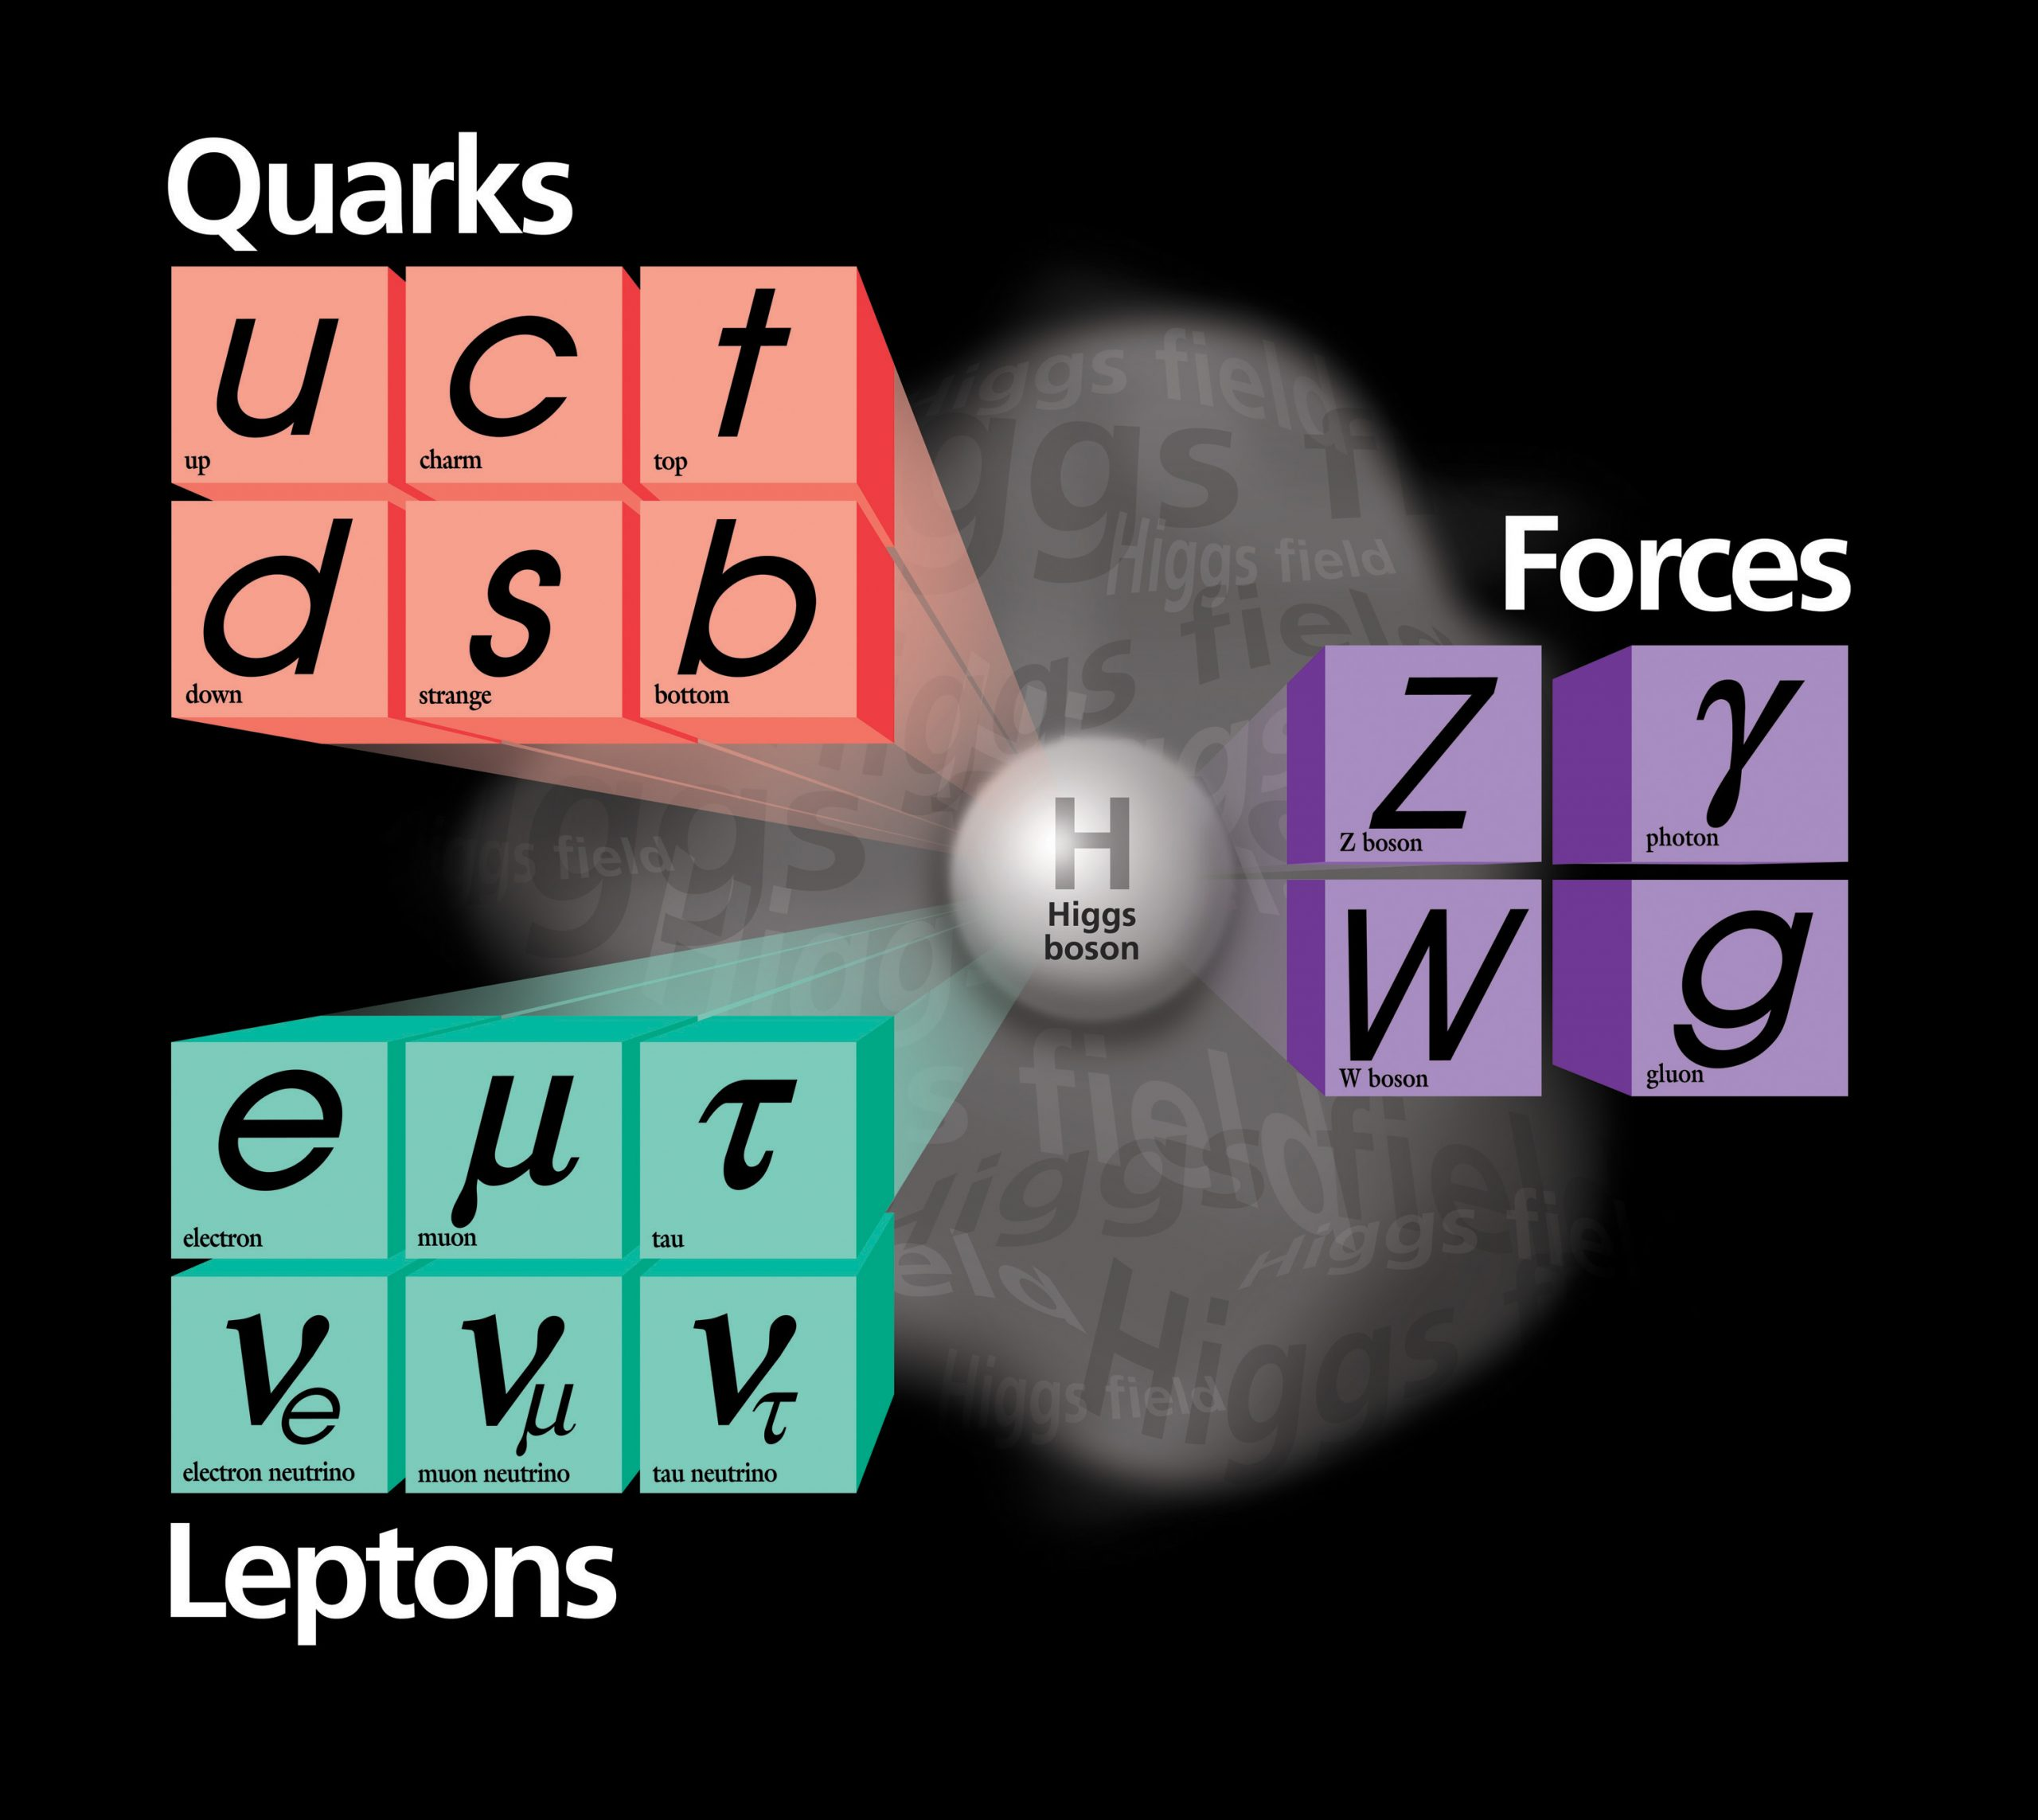
\includegraphics[height=10cm, width=10cm]{pictures/SM.jpg}
 \label{fig:1.1}
\end{figure}

标准模型共有61种基本粒子(见\textbf{表\ref{table:1.1}}),包含费米子及玻色子——费米子为拥有半奇数的自旋并遵守泡利不相容原理的粒子;玻色子则拥有整数自旋并且不遵守泡利不相容原理。简单来说,费米子就是组成物质的粒子而玻色子则负责传递各种作用力。

基本粒子中所有费米子自旋都为$\frac{1}{2}$,包括三代夸克及其反粒子,三代轻子及其反粒子,正反粒子具有相同的质量和相反的电荷。基本粒子中W,Z,光子传播电弱相互作用,自旋都为1;胶子传播强相互作用,自旋也为1;希格斯粒子自旋为0,通过Yukawa相互作用与粒子耦合并赋予它们质量。

值得一提的是,所有下型轻子(也就是中微子,包括电子中微子$\nu_e$,缪子中微子$\nu_\mu$,陶子中微子$\nu_\tau$)电荷为0且无色荷,所以不能参与电磁相互作用和强相互作用,只能参与难以直接探测的弱相互作用,只能通过量能器的能量沉积得到击中信息,并且很多时候根本探测不到,所以在实验中也经常被称为“消失的中性粒子”。
\begin{table}[htbp]
    \caption{基本粒子}\label{table:1.1}
    \centering
    \begin{tabular}{>{\centering\arraybackslash}p{1.5cm}%
    >{\centering\arraybackslash}p{2cm}%
    >{\centering\arraybackslash}p{2cm}%
    >{\centering\arraybackslash}p{1.5cm}%
    >{\centering\arraybackslash}p{2cm}%
    >{\centering\arraybackslash}p{2cm}%
    >{\centering\arraybackslash}p{1.5cm}}
    \toprule\toprule
    \textbf{名称} & \textbf{自旋类型} & \textbf{同位旋数(上下型)} & \textbf{世代数} & \textbf{电荷种类(正反粒子)} & \textbf{色荷种类} & \textbf{总计}\\
    \midrule
    夸克 & 半整数 & 2 & 3 & 2 & 3 & 36\\
    轻子 & 半整数 & 2 & 3 & 2 & \diagbox[height=0.6\line] & 12\\
    胶子 & 整数 & 1 & 1 & 1 & 8 & 8\\
    W & 整数 & 1 & 1 & 2 & \diagbox[height=0.6\line] & 2\\
    Z & 整数 & 1 & 1 & 1 & \diagbox[height=0.6\line] & 1\\
    光子 & 整数 & 1 & 1 & 1 & \diagbox[height=0.6\line] & 1\\
    希格斯 & 整数 & 1 & 1 & 1 & \diagbox[height=0.6\line] & 1\\
    \midrule
    总计 & & & & & & 61\\
    \bottomrule\bottomrule
\end{tabular}
\end{table}




\subsection{标准模型的相互作用}
\subsubsection{强相互作用}
强相互作用由$SU(3)_c$群的量子色动力学(QCD)描述,该群的生成元是8个线性无关矩阵$T^a=\frac{\lambda^a}{2}$,其中$\lambda^a$是Gell-Mann矩阵,a表示着8个色自由度,为了保证规范不变性,需要引入协变微分
\begin{equation}
    \left( D_\mu \right)_{ij} = \partial_\mu \delta_{ij} - i g \left( T_a \right)_{ij} \mathcal{A}^a_\mu
\end{equation}
将拉氏量改写为
\begin{equation}
    \mathcal{L}_\mathrm{QCD} = \bar{\psi}_i  \left( i \gamma^\mu (D_\mu)_{ij} - m\, \delta_{ij}\right) \psi_j - \frac{1}{4}G^a_{\mu \nu} G^{\mu \nu}_a
\end{equation}
这里的G表示为规范不变胶子场强度张量
\begin{equation}
    G^a_{\mu \nu} = \partial_\mu \mathcal{A}^a_\nu - \partial_\nu \mathcal{A}^a_\mu + g f^{abc} \mathcal{A}^b_\mu \mathcal{A}^c_\nu
\end{equation}
其中${\mathcal {A}}_{\mu }^{a}(x)$是胶子场。

根据量子场论的规则和相关的费曼图,上述理论产生了三种基本相互作用:一个夸克可以发射(或吸收)一个胶子,一个胶子可以发射(或吸收)一个胶子,以及两个胶子可以直接互动。这与QED形成对比,在 QED 中只发生第一种相互作用,因为光子没有电荷。

使用上述拉氏量的详细计算表明,介子中夸克与其反夸克之间的有效势包含一项与夸克和反夸克之间的距离成比例增加的项($\prop r$ ),它表示粒子与其反粒子在远距离相互作用的某种“刚度”,类似于橡皮筋的熵弹性。这导致夸克被限制在强子内部,即介子和核子,具有特征半径$R_c\sim\SI{1}{fm}(=10^{-15}\si{m})$。

\subsubsection{电弱相互作用}
在粒子物理学中,电弱相互作用是电磁相互作用与弱相互作用的统一描述,而这两种作用都属于自然界中四种已知基本相互作用。在粒子物理的[GeV]及以下能标中,电磁作用与弱作用存在很大的差异,然而在能标超过W的不变质量,即至少在100[GeV]的能标下,这两种作用力会统一成的电弱相互作用。

数学上是用一个SU(2)×U(1)的规范群统一描述电磁作用及弱作用。当中对应的零质量规范玻色子分别是三个来自SU(2)弱同位旋的W玻色子($W^+$、$W_0$和$W^−$
)以及一个来自U(1)弱超荷的$B_0$玻色子。

在标准模型里$W^±$和$Z_0$玻色子和光子是经由$SU(2)\otimes U(1)_Y$的电弱对称性自发对称破缺成$U(1)_{em}$所产生的,此一过程称作希格斯机制(见希格斯玻色子)。$U(1)_Y$和$U(1)_{em}$都属于$U(1)$群,但两者不同;$U(1)_{em}$的生成元是电荷$Q=Y/2+I_3$,而其中Y是$U(1)_Y$(叫弱超荷)的生成元,$I_3$(弱同位旋的一个分量)则是$SU(2)$的其中一个生成元。

属于$SU(2)\otimes U(1)_Y$自由费米子场的拉氏量如下
\begin{equation}
    \mathscr{L}=i\Bar{\Psi}\gamma^\mu\partial_\mu \Psi
\end{equation}
为了满足场在$SU(2)\otimes U(1)_Y$规范变换下的局域不变性,我们必须得引入协变微商$\mathcal{D}_\mu$以代替$\partial_\mu$:
\begin{equation}
    \mathcal{D}_\mu=\partial_\mu -i\frac{g}{2}gT^aW_\mu^a-i\frac{g^\prime}{2} Y B_\mu
\end{equation}
其中$g$为$SU(2)_L$作用的耦合常数,$g^\prime$为$U(1)_Y$作用的耦合常数,T是弱同位旋矩阵,形式上等同于泡利矩阵,a是欧式指标可取1,2,3(度量矩阵为3阶单位阵),$\mu$、$\nu$是四维指标。
从而将带电弱相互作用的费米子场拉氏量改写为
\begin{equation}
    \mathscr{L}=i\Bar{\Psi}\gamma^\mu\mathcal{D}_\mu \Psi-\frac{1}{4}W^{\mu\nu}_a W^a_{\mu\nu}-\frac{1}{4}B^{\mu\nu}B_{\mu\nu}
\end{equation}
其中有三个带电的无质量玻色子$W^1,W^2,W^3$和一个无质量的中性玻色子B,由于对称性自发破缺,将会出现我们实验中观测到的有质量正负W玻色子,可表示为
\begin{equation}
    W^{\pm}=\frac{1}{\sqrt{2}}(W^1\mp iW^2)
\end{equation}
相应地,Z和$\gamma$光子可表示为
\begin{equation}
    \begin{pmatrix}
\gamma \\
Z \end{pmatrix} = \begin{pmatrix}
\cos \theta_\text{W} & \sin \theta_\text{W} \\
-\sin \theta_\text{W} & \cos \theta_\text{W} \end{pmatrix} \begin{pmatrix}
B \\
W_3 \end{pmatrix}
\end{equation}
其中$\theta_W$是电弱混合角,也被称为温伯格角。

\subsubsection{引入质量耦合的Higgs机制}
上面提到电弱统一中本来是无质量的$W^1,W^2$可通过自发对称破缺变为有质量的$W^\pm$,这就是通过希格斯机制实现的质量赋予。

因为电弱统一是$SU(2)\otimes U(1)$理论,讨论起来较为复杂,所以我们从U(1)群的希格斯机制开始讨论。

因为我们知道自旋为0质量为m的粒子的拉氏量为
\begin{equation}
    \mathcal{L}=(\partial_{\alpha} \phi)^*(\partial^{\alpha} \phi)-m^2\phi^*\phi -V(\phi^*\phi)
\end{equation}
反过来,如果一个拉氏量中有$\phi$的二阶项,那么它的系数就可以认为是场对应粒子的不变质量。

现在让我们考虑一个无质量标量场$\phi$,并将该场的拉氏量写为
\begin{equation}\label{eq:1.1}
    \mathcal{L}=\partial_{\mu}\bar{\phi}\partial^{\mu} \phi+\mu^2\bar{\phi}\phi -\lambda(\bar{\phi}\phi)^2
\end{equation}
其中$\lambda$,$\mu$都大于0,希格斯势为$V=\lambda\bar{\psi}\psi)^2-\mu^2\bar{\psi}\psi$,该拉氏量满足$U(1)$的局域对称变换。显然这个类二次函数的最低值在$\bar{\phi}\phi\frac{|v|^2}{2}=\frac{-\mu^2}{2\lambda}$处(其中$v=\frac{\mu}{\sqrt{\lambda}}$也就是量子场论中的真空态),在$\phi$二维复平面上考虑$V$的高度就可以形成一个旋转对称墨西哥草帽的形状。

我们现在将原始的$\phi$写成$\phi=\phi_1+i\phi_2=(\varphi_1+v+i\varphi_2)/\sqrt{2}$,其中$v=\frac{\mu}{\sqrt{\lambda}}$当成真空态,$(\varphi_1+i\varphi_2)/\sqrt{2}$才当成我们现在要考虑的$U(1)$相互作用的粒子,我们知道$U(1)$相互作用的协变微分可以写为$\mathcal{D}_\mu=\partial_{\mu}+iqA_{\mu}$,把以上结果代入$U(1)$相互作用的拉氏量有
\begin{equation}
\begin{aligned}\mathcal{L} & =\frac{1}{2}[(\partial_{\alpha}+iqA_{\alpha})(\varphi_1+v+i\varphi_2)]^*
[(\partial^{\alpha}+iqA^{\alpha})(\varphi_1+v+i\varphi_2)]
-\ \frac{1}{4}F_{\alpha\beta}F^{\alpha\beta} \\
 & \qquad+\frac{\mu^2}{2}(\varphi_1+v+i\varphi_2)^*(\varphi_1+v+i\varphi_2)
-\ \frac{\lambda}{4}[(\varphi_1+v+i\varphi_2)^*(\varphi_1+v+i\varphi_2)]^2 \\
\end{aligned}
\end{equation}
化简后有
\begin{equation}
    \mathcal{L}=\frac{1}{2}(\partial_{\alpha}\varphi_1)(\partial^{\alpha}\varphi_1)
-\mu^2\varphi_1^2+\ \frac{1}{2}(\partial_{\alpha}\varphi_2)(\partial^{\alpha}\varphi_2)-\ \frac{1}{4}F_{\alpha\beta}F^{\alpha\beta} +\ \frac{1}{2}q^2 v^2 A_{\alpha}A^{\alpha}+ \mathcal{L}_{int}
\end{equation}

又因为$U(1)$对称性要求拉氏量在$\phi\to e^{i\theta(x)}\phi$旋转变换下不变,于是我们在局域变换中设定相位$\theta=-\arctan{(\phi_2/\phi_1)}$,并令$\phi\to \phi'=e^{i\theta}\phi=(\phi_1\cos{\theta}-\phi_2\sin{\theta})
+i(\phi_1\sin{\theta}+\phi_2\cos{\theta})$即可得到
\begin{equation}
    \mathcal{L}=\ \frac{1}{2} (\partial_{\alpha}\varphi_1)(\partial^{\alpha}\varphi_1) 
-\mu^2\varphi_1^2  -\ \frac{1}{4}F_{\alpha\beta}F^{\alpha\beta} +\ \frac{1}{2}q^2 v^2 A_{\alpha}A^{\alpha} +\mathcal{L}_{int}
\end{equation}
其中$F_{\alpha\beta}=\partial_\alpha A_\beta-\partial_\beta A_\alpha$

现在我们得到,$\varphi_1$是赋予质量的希格斯粒子场,其质量为$\sqrt{2}\mu$,$U(1)$规范矢量场$A_\alpha$的质量为$|q|\mu/\sqrt{\lambda}$,为对应规范玻色子的质量。

对于$SU(2)\otimes U(1)$群,希格斯场从$\varphi_1$变为了复值的
\begin{equation}
    \phi (x) ={\left ( \begin{matrix} \phi_1 + \mathrm{i} \phi_2\\ \phi_3 + \mathrm{i} \phi_4 \end{matrix} \right )}
\end{equation}
通过对称性自发破缺,产生了三个带质量的玻色子$W^\pm,Z$和一个无质量玻色子$\gamma$。

\section{超出标准模型的迹象}
\subsection{g-2实验结果与标准模型理论值的偏差}
$\mu$子是一种类似于电子的基本粒子,和电子一样带有一个单位负电荷、自旋为1/2,但具有更大的质量,$\mu$子的质量大约是电子的200倍。$\mu$子与同属于轻子的电子和$\tau$子具有相似的性质,人们至今未发现轻子具有任何内部结构。

像电子一样,$\mu$子的行为就好像它们有一个微小的内部磁铁。在强磁场中,$\mu$子磁铁的方向会进动或摆动,就像陀螺或陀螺仪的轴一样。内部磁铁的强度决定了 $\mu$ 子在外部磁场中进动的速率,我们用称为“g因子”的参数表示这块“磁铁”的强度和旋转速度。这个数字可以用量子场论进行超高精度计算。对于标准模型中的费米子,普适的g的物理定义是
\begin{equation}
    \boldsymbol \mu = g {e \over 2m} \mathbf S 
\end{equation}
其中e是单位电荷大小,m是基本粒子不变质量,$\mathbf S $是自旋,$\boldsymbol\mu$是磁矩。按照狄拉克方程的计算,基本费米子的g=2。

当宇宙射线撞击地球大气层时会自然产生$\mu$子,费米实验室的粒子加速器可以大量产生它们。

根据量子场论的计算(由于真空态和量子涨落),对于$\mu$子,g的值略大于 2,我们主要关心g和2的差异,因此得名“g-2”实验。这种与2的差异是由量子场论的高阶贡献引起的。在高精度测量g-2并将其值与理论预测进行比较时,物理学家将发现实验是否与理论相符。任何超过误差允许的偏差都会暗示着自然界中存在尚未发现的亚原子粒子。

2021年,美国费米国家实验室的 Muon g-2 实验备受期待的首个结果表明,在前所未有的精确度测量下,$\mu$子的g因子与标准模型计算结果存在较大偏差。几十年来,g-2的实验和理论差异就已经被测量过,这个里程碑式的结果,更是进一步确认了这个差异。

当 $\mu$子在费米实验室的Muon\ g-2磁铁中绕圈旋转时,它们同时会与与量子涨落不断生成或湮灭的亚原子粒子相互作用。与这些短寿命粒子的相互作用会影响 g 因子的值,导致 $\mu$子的进动加速或减速非常轻微。标准模型极其精确地预测了这种所谓的异常磁矩。但是,如果量子涨落中包含标准模型未考虑的额外相互作用力或粒子,那将进一步影响$\mu$子的g因子大小。

公认的$\mu$子g因子理论值为:g=2.00233183620(86)。而费米实验室的Muon\ g-2 实验宣布的新实验结果为:g=2.00233184122(82)。(见下\textbf{图\ref{fig:1.2}})
\begin{figure}[H]
 \centering
 \caption{g因子的标准模型理论值与实验的偏差}
 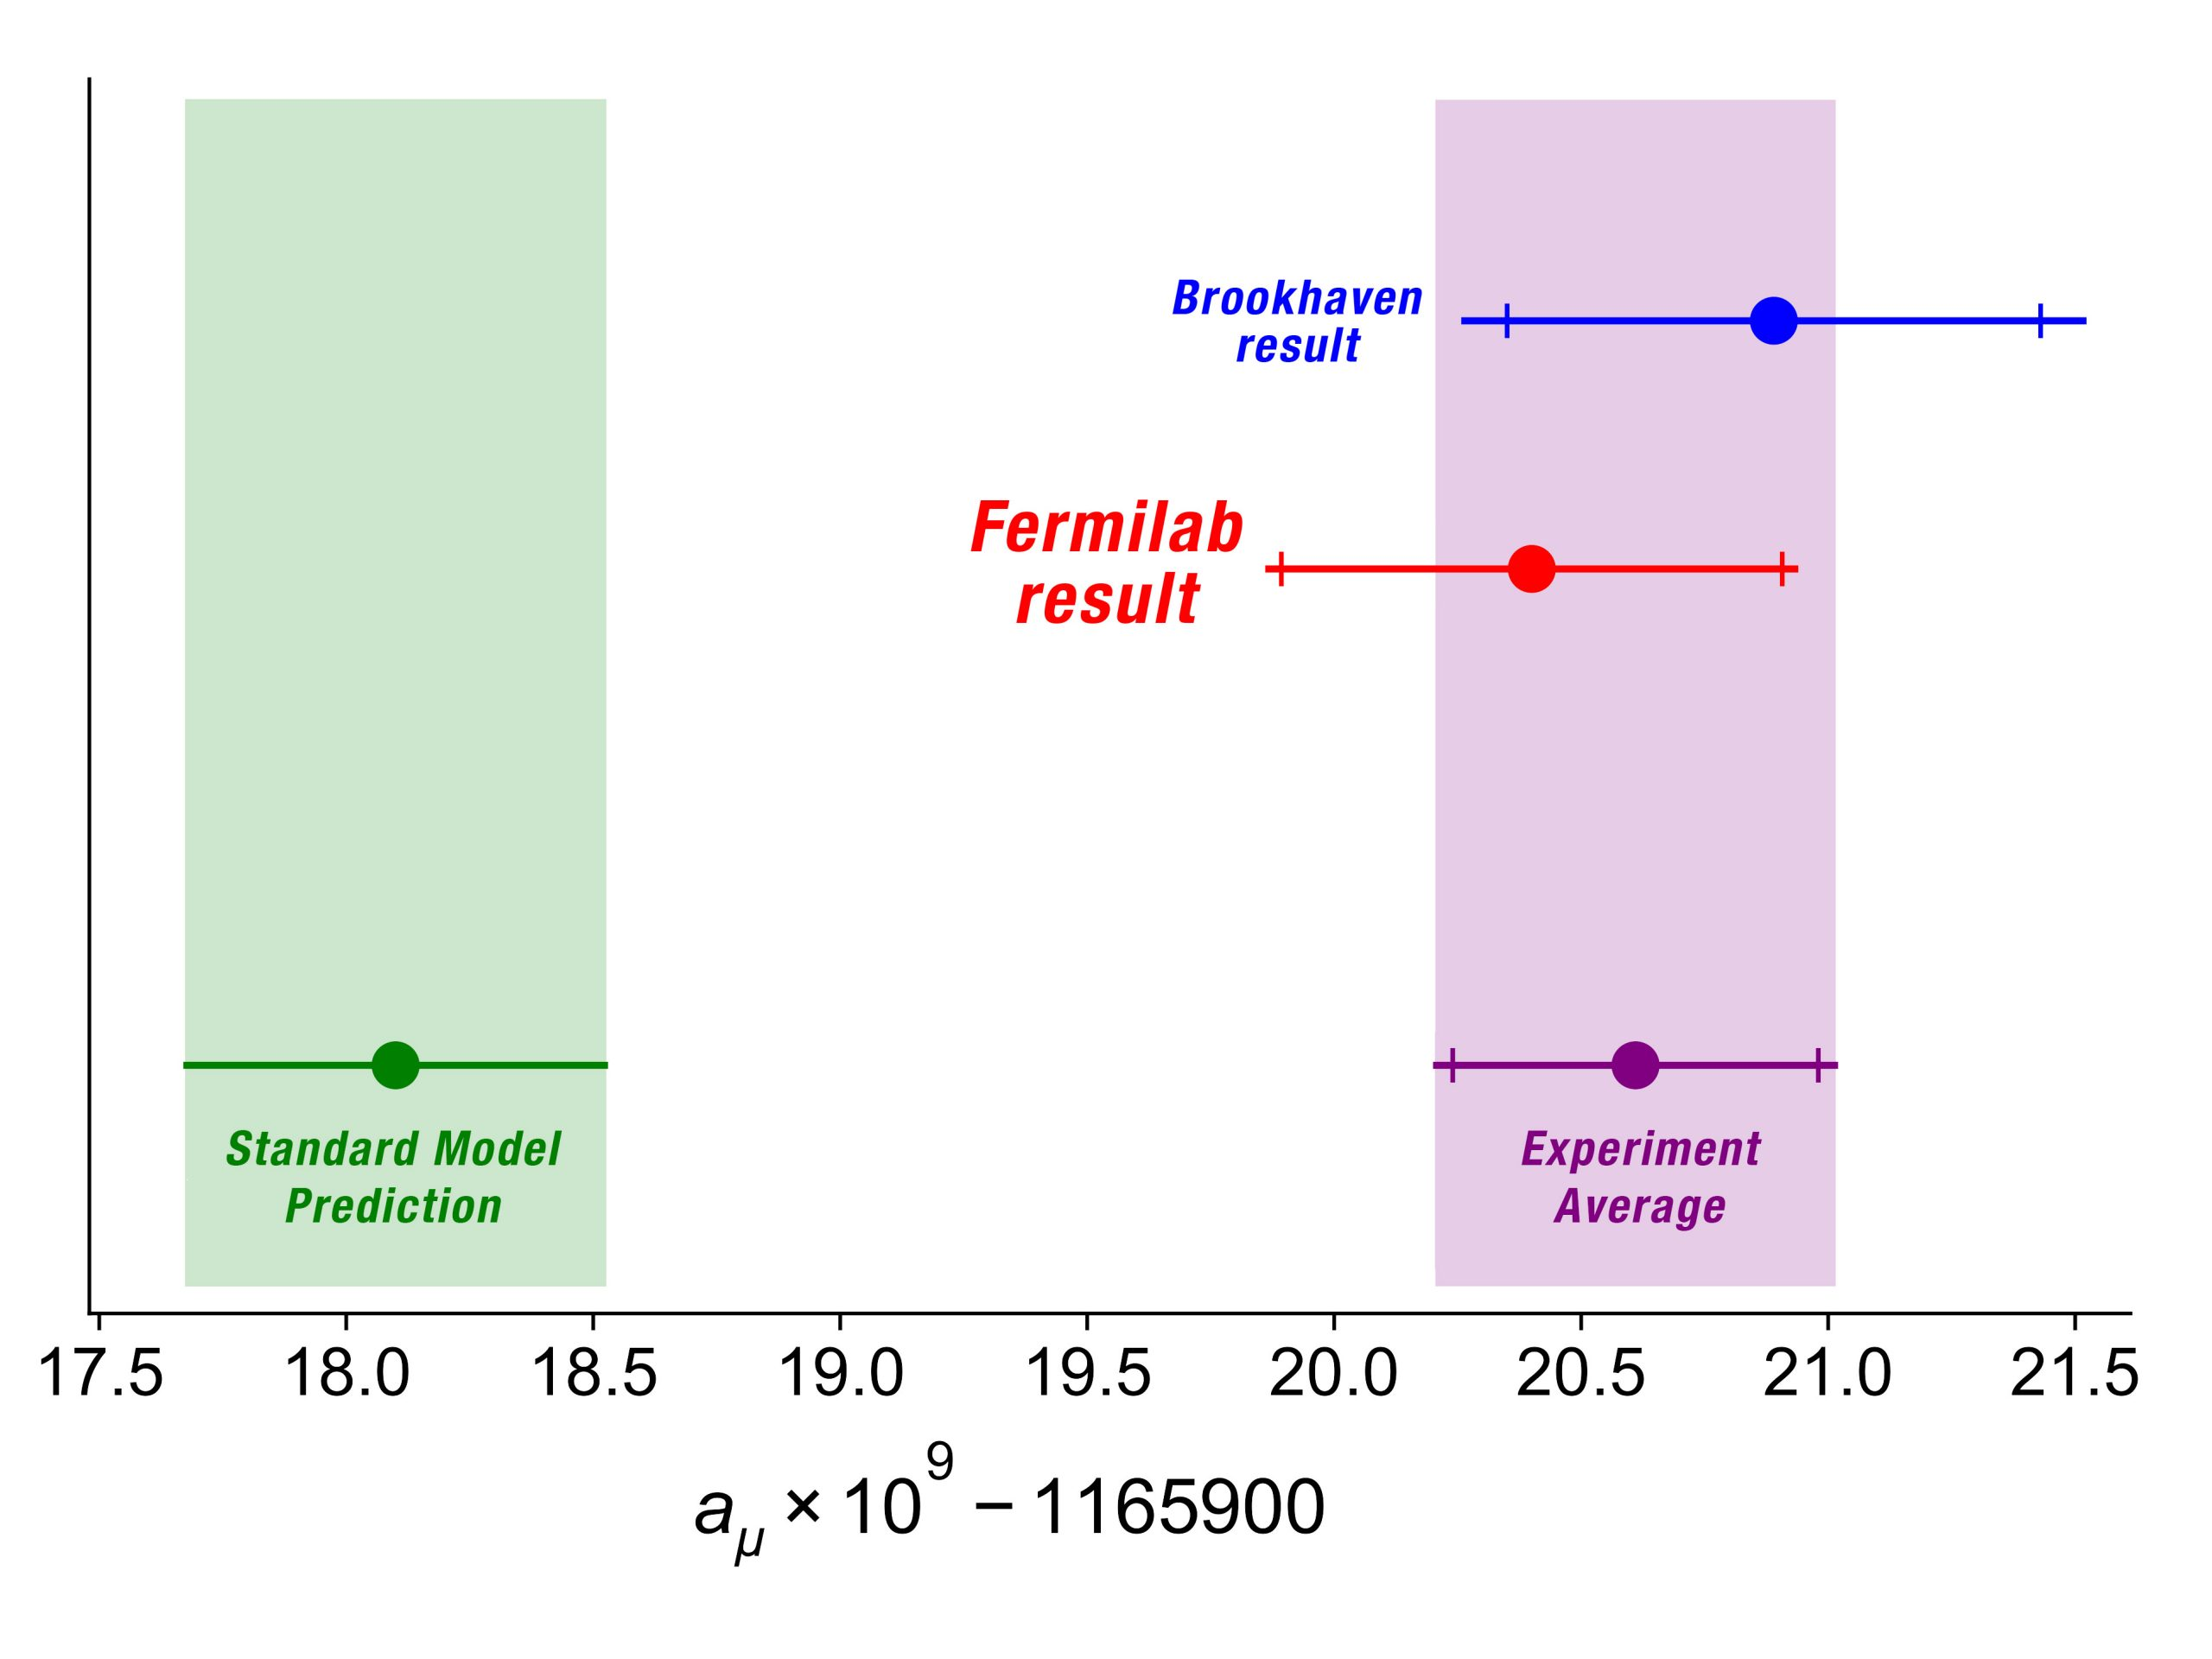
\includegraphics[height=10cm, width=12cm]{pictures/Muon-g-2-results-plot.jpeg}
 \label{fig:1.2}
\end{figure}

费米实验室和布鲁克海文的联合结果显示,实验测量与理论的差异显著度为$4.2\sigma$(标准偏差),尽管略低于公认具有说服力的新物理证据所需的$5\sigma$阈,但$4.2\sigma$表明这次与标准模型的冲突结果是统计涨落的可能性约为四万分之一。

在 2018 年运行的第一年,费米实验室收集的数据比之前所有$\mu$子g因子实验的总和还要多。目前已完成对第一次运行中超过 80 亿个 $\mu$ 子的运动的分析。正在进行第二次和第三次实验的数据分析,第四次正在进行中,第五次正在计划中。到目前为止,只分析了不到 6\% 的实验最终将收集的数据。结合所有五次运行的结果,$\mu$子的g因子将得到更加精确地测量,从而更确定地揭示新物理是否隐藏在量子涨落中。

\subsection{超重的W玻色子}
W玻色子是弱相互作用的媒介粒子。它参与太阳发光和粒子衰变的反应过程。标准模型给出的W质量理论计算值为$M_W=(80357\pm6)$MeV。(该值基于复杂的标准模型计算,该计算通过将 W 玻色子的质量与其他两个粒子的质量的测量错综复杂地联系起来:顶夸克,于 1995 年在费米实验室的 Tevatron 对撞机中发现;希格斯玻色子,在2012 年欧洲核子研究中心的大型强子对撞机上发现)

过去 40 年来,许多对撞机实验都对W玻色子质量进行了测量,这些测量都是具有挑战性和十分复杂的。但是2022年4月公布的美国费米国家实验室的W质量测量达到了更高的精度——经过 10 年的仔细分析和审查,美国能源部费米国家加速器实验室与 CDF 合作的科学家今天宣布,他们已经实现了迄今为止对 W 玻色子质量的最精确测量。

利用费米实验室的Tevatron对撞机产生的高能粒子碰撞和对撞机探测器(CDF)收集的数据,研究人员收集了1985年至2011年间包含W玻色子的大量数据,它基于对 420 万个 W 玻色子候选者的观察,大约是2012年发布的合作分析中使用的数量的四倍。并且花了十年的时间来完成所有的细节和必要的检查,科学家们现在已经以 0.01\%的精度确定了粒子的质量(是之前最佳测量精度的两倍),得到了迄今为止精度最可靠的测量结果:$M_W=(80433.5\pm 9.4)$MeV。(见\textbf{图\ref{fig:1.3}})
\begin{figure}[H]
 \centering
 \caption{不同实验对W质量测量结果的比较\cite{Wmass}}
 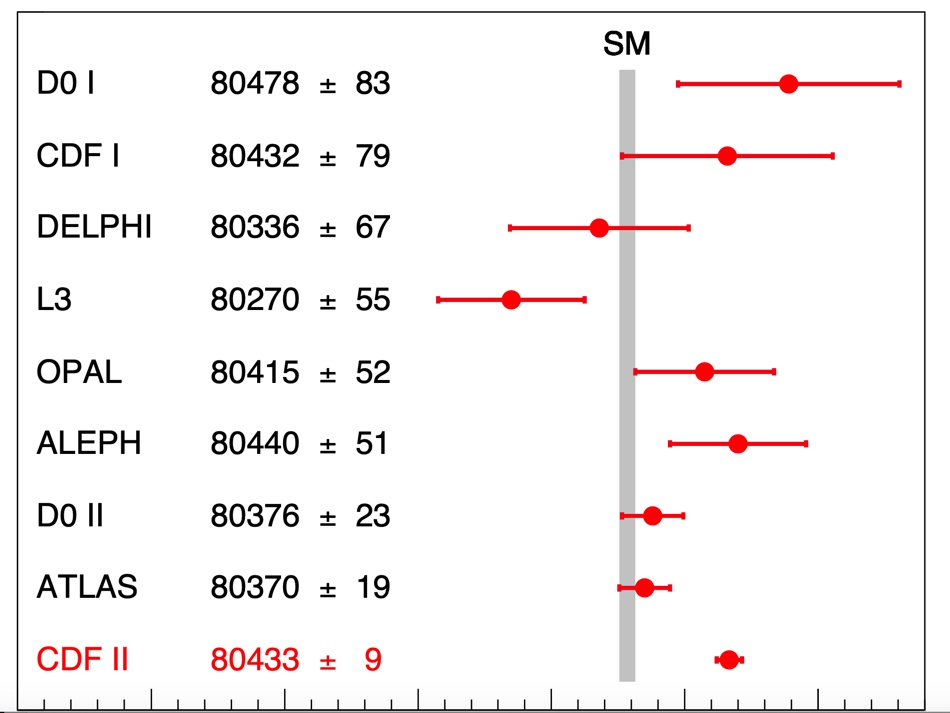
\includegraphics[height=10cm, width=12cm]{pictures/w-boson-comparisons.jpeg}
 \label{fig:1.3}
\end{figure}

通过合成以上两个数据的独立不确定度,我们可以得到测量值和标准模型预期值之间的差异存在$7\sigma$的偏差。这显示出了标准模型框架下,理论和实验的值产生了聚大冲突。如果无潜在错误,此测量表明可能需要改进标准模型计算或扩展模型。

科学界对这个结果也是众说纷纭——费米实验室副主任Joe Lykken指出:“虽然这是一个有趣的结果,但测量结果需要通过另一个实验来确认,然后才能完全解释。”
德克萨斯农工大学CDF联合发言人David Toback补充道:“如果实验值和预期值之间的差异是由于某种新的粒子或亚原子相互作用造成的,这是一种可能性,那么它很有可能在未来的实验中被发现。”

\section{LHC上的CMS实验}
\subsection{大型强子对撞机(LHC)}
大型强子对撞机(LHC)是世界上最大、能量最高的粒子对撞机。它由欧洲核研究组织(CERN)于1998年至2008年间与 10000多名科学家、数百所大学和实验室以及 100多个国家合作建造。它位于日内瓦附近法国-瑞士边界下方的一条周长27公里(17 英里)、深达175米(574英尺)的隧道中。

\begin{figure}[H]
 \centering
 \caption{LHC的探测器和部门分布}
 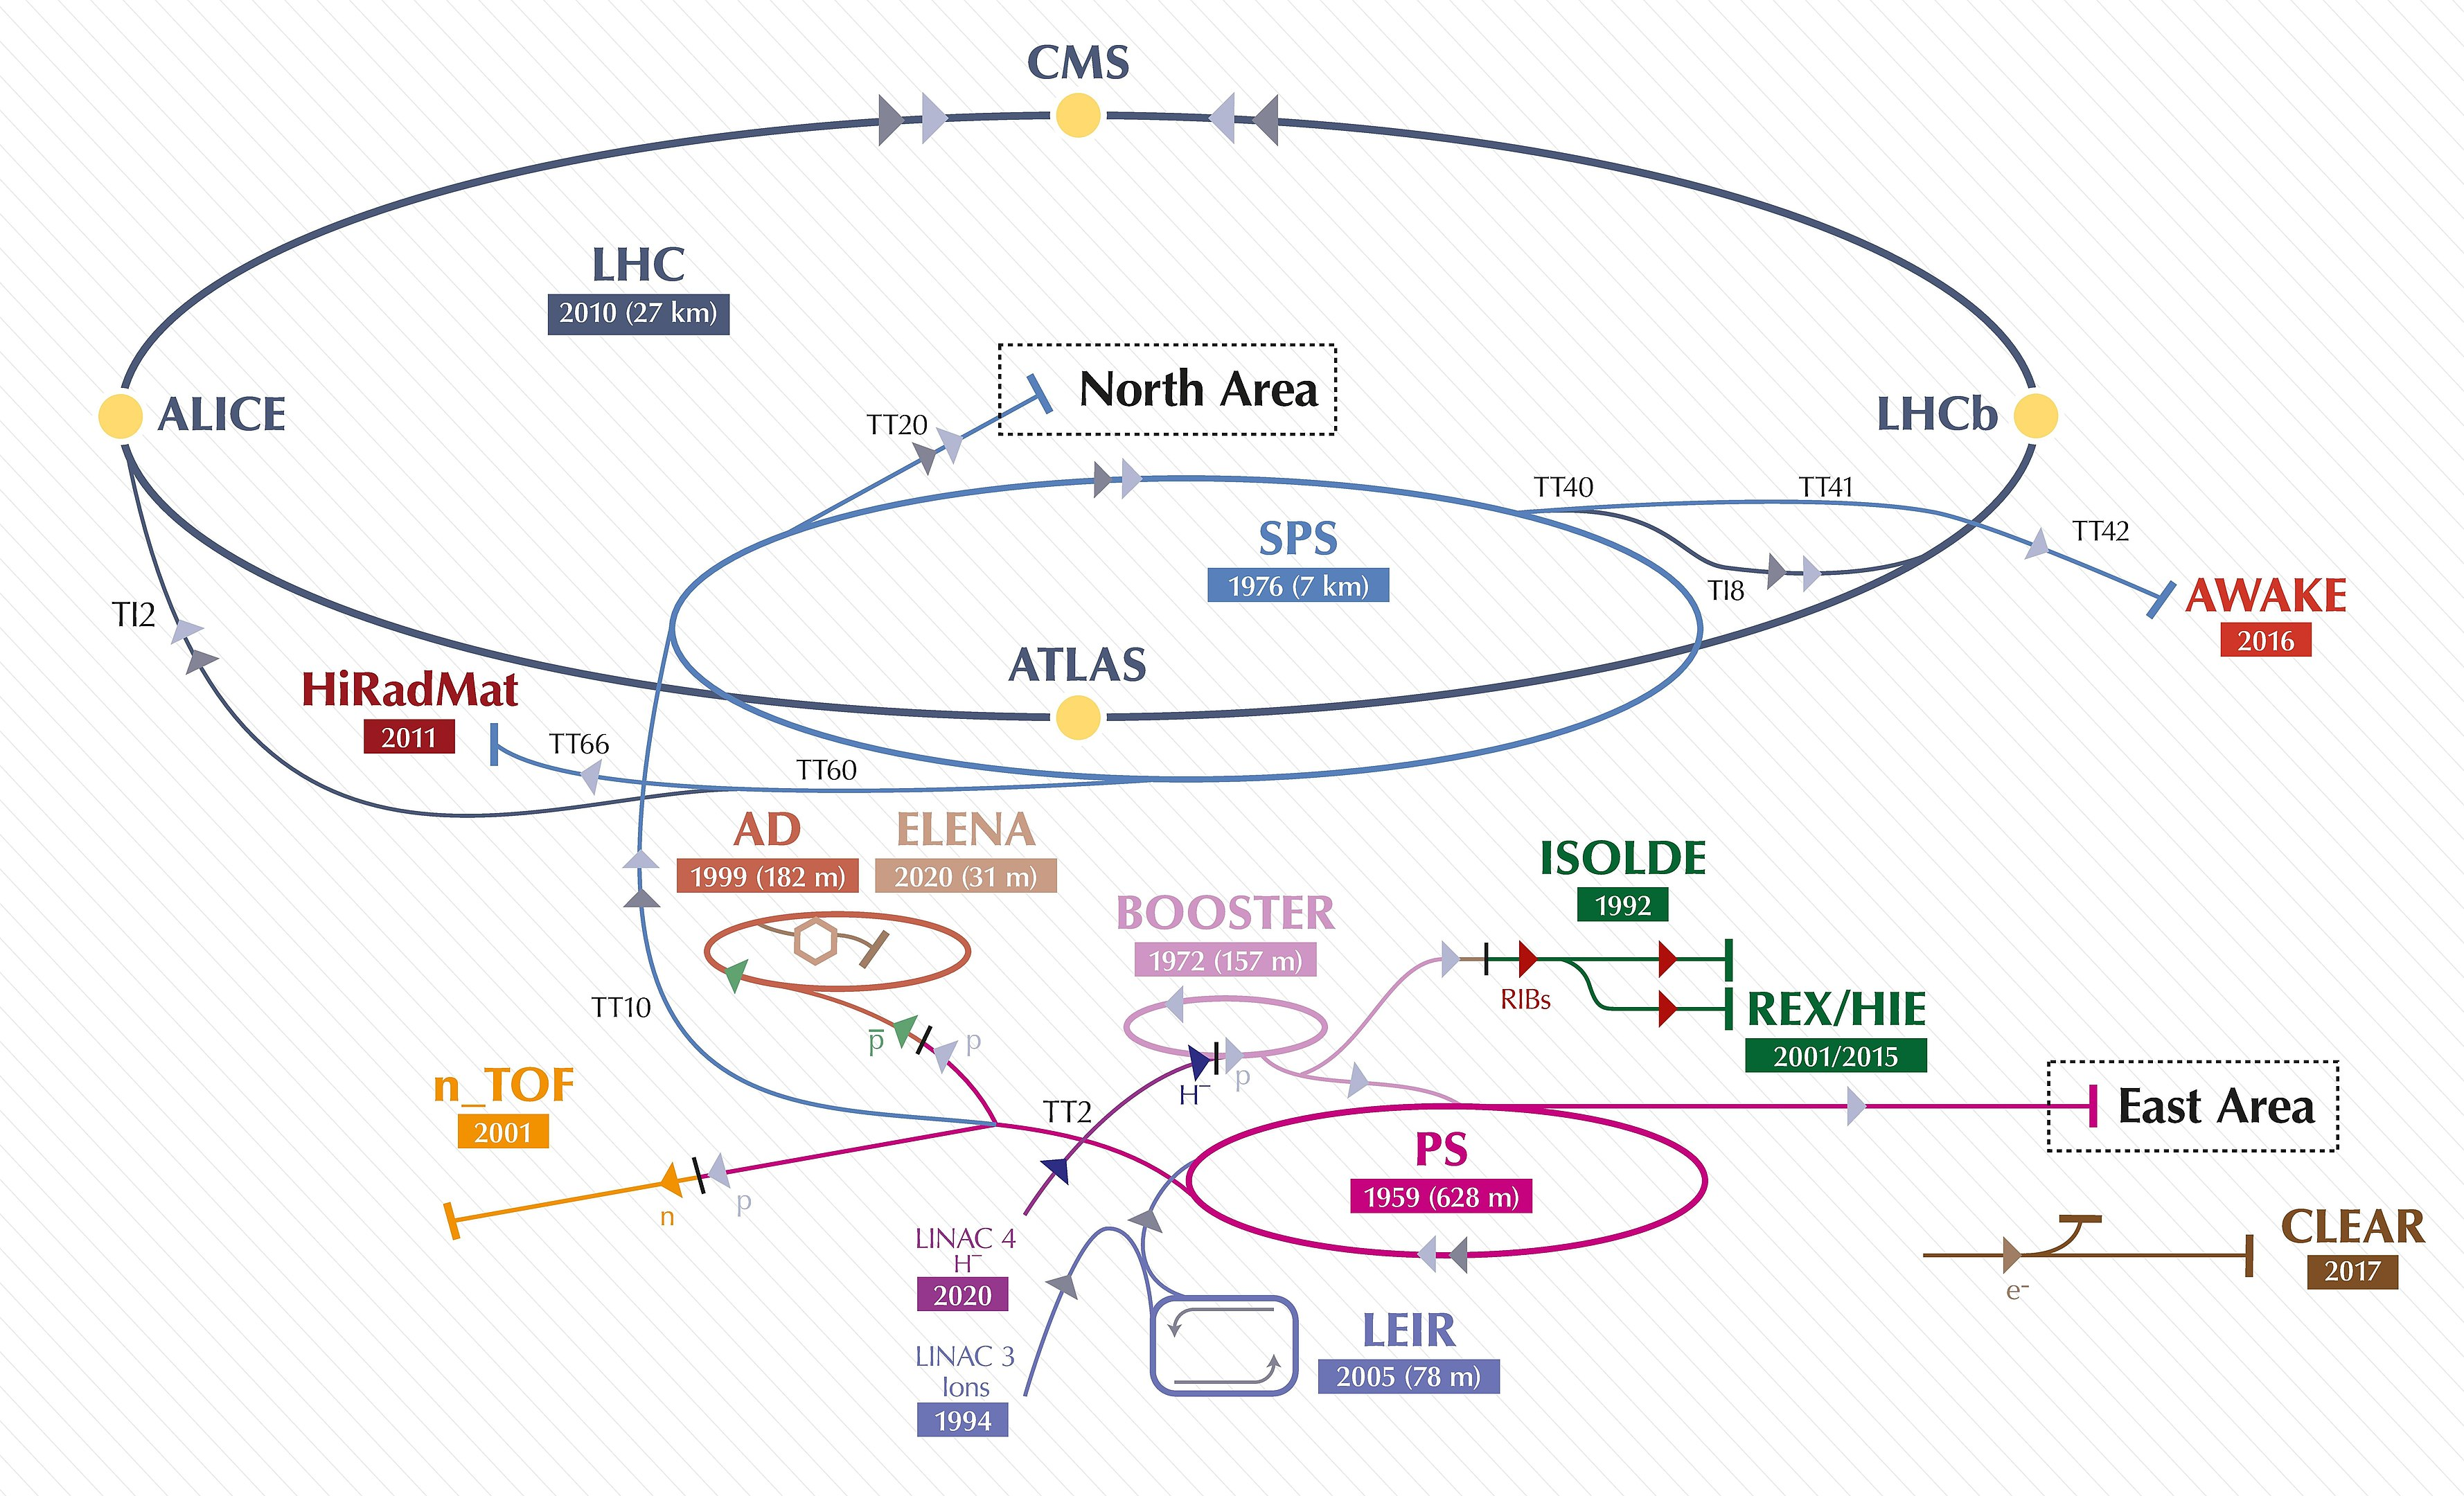
\includegraphics[height=8cm, width=14cm]{pictures/CERN_accelerator_complex_(cropped_2).jpeg}
 \label{fig:1.4}
\end{figure}

LHC上的第一轮运行(RUN I)开始于2010年每个质子束3.5TeV的能量对撞,约为之前世界纪录的四倍。升级后,RUN II达到每质子束6.5TeV(总碰撞能量13TeV,目前世界最高)。 2018年底停产三年,正在进一步升级到RUN III。

LHC上有四个交叉点,加速粒子在这些交叉点发生碰撞。LHC还有七个探测器,每个设用于检测不同的现象,位于交叉点周围。LHC主要碰撞质子束,但它也可以加速重离子束:铅-铅碰撞和质子-铅碰撞通常每年进行一个月。

LHC的目标是让物理学家能够测试不同粒子物理理论的预测,包括测量希格斯玻色子的性质,寻找超对称理论和其他未解决的粒子物理问题。

\subsection{紧凑缪子螺线管实验(CMS)}
紧凑型介子螺线管(CMS)实验是在瑞士和法国欧洲核子研究中心的大型强子对撞机(LHC) 上建造的两个大型通用粒子物理探测器之一。CMS实验的目标是研究广泛的物理学,包括寻找希格斯玻色子、额外维度和可能构成暗物质的粒子。

CMS长21m,直径15m,重约14000吨。来自47个国家/地区的206个科研机构的4000 多人组成的CMS合作组建造并运行了探测器。2012年7月,CMS与ATLAS一起初步发现了希格斯玻色子。

CMS实验的主要目标是:
\begin{itemize}
    \item 在TeV尺度上探索物理学
    \item 进一步研究CMS和ATLAS已经发现的希格斯玻色子的性质
    \item 寻找超出标准模型的物理证据,例如超对称或额外维度
    \item 研究重离子碰撞的各个方面
\end{itemize}

位于LHC环另一侧的ATLAS实验的设计考虑了相似的目标,这两个实验旨在相互补充,以扩大范围并提供对研究结果的证实。CMS和ATLAS使用不同的技术解决方案和探测器磁铁系统设计来实现目标。



\begin{figure}[H]
 \centering
 \caption{CMS探测器剖面图}
 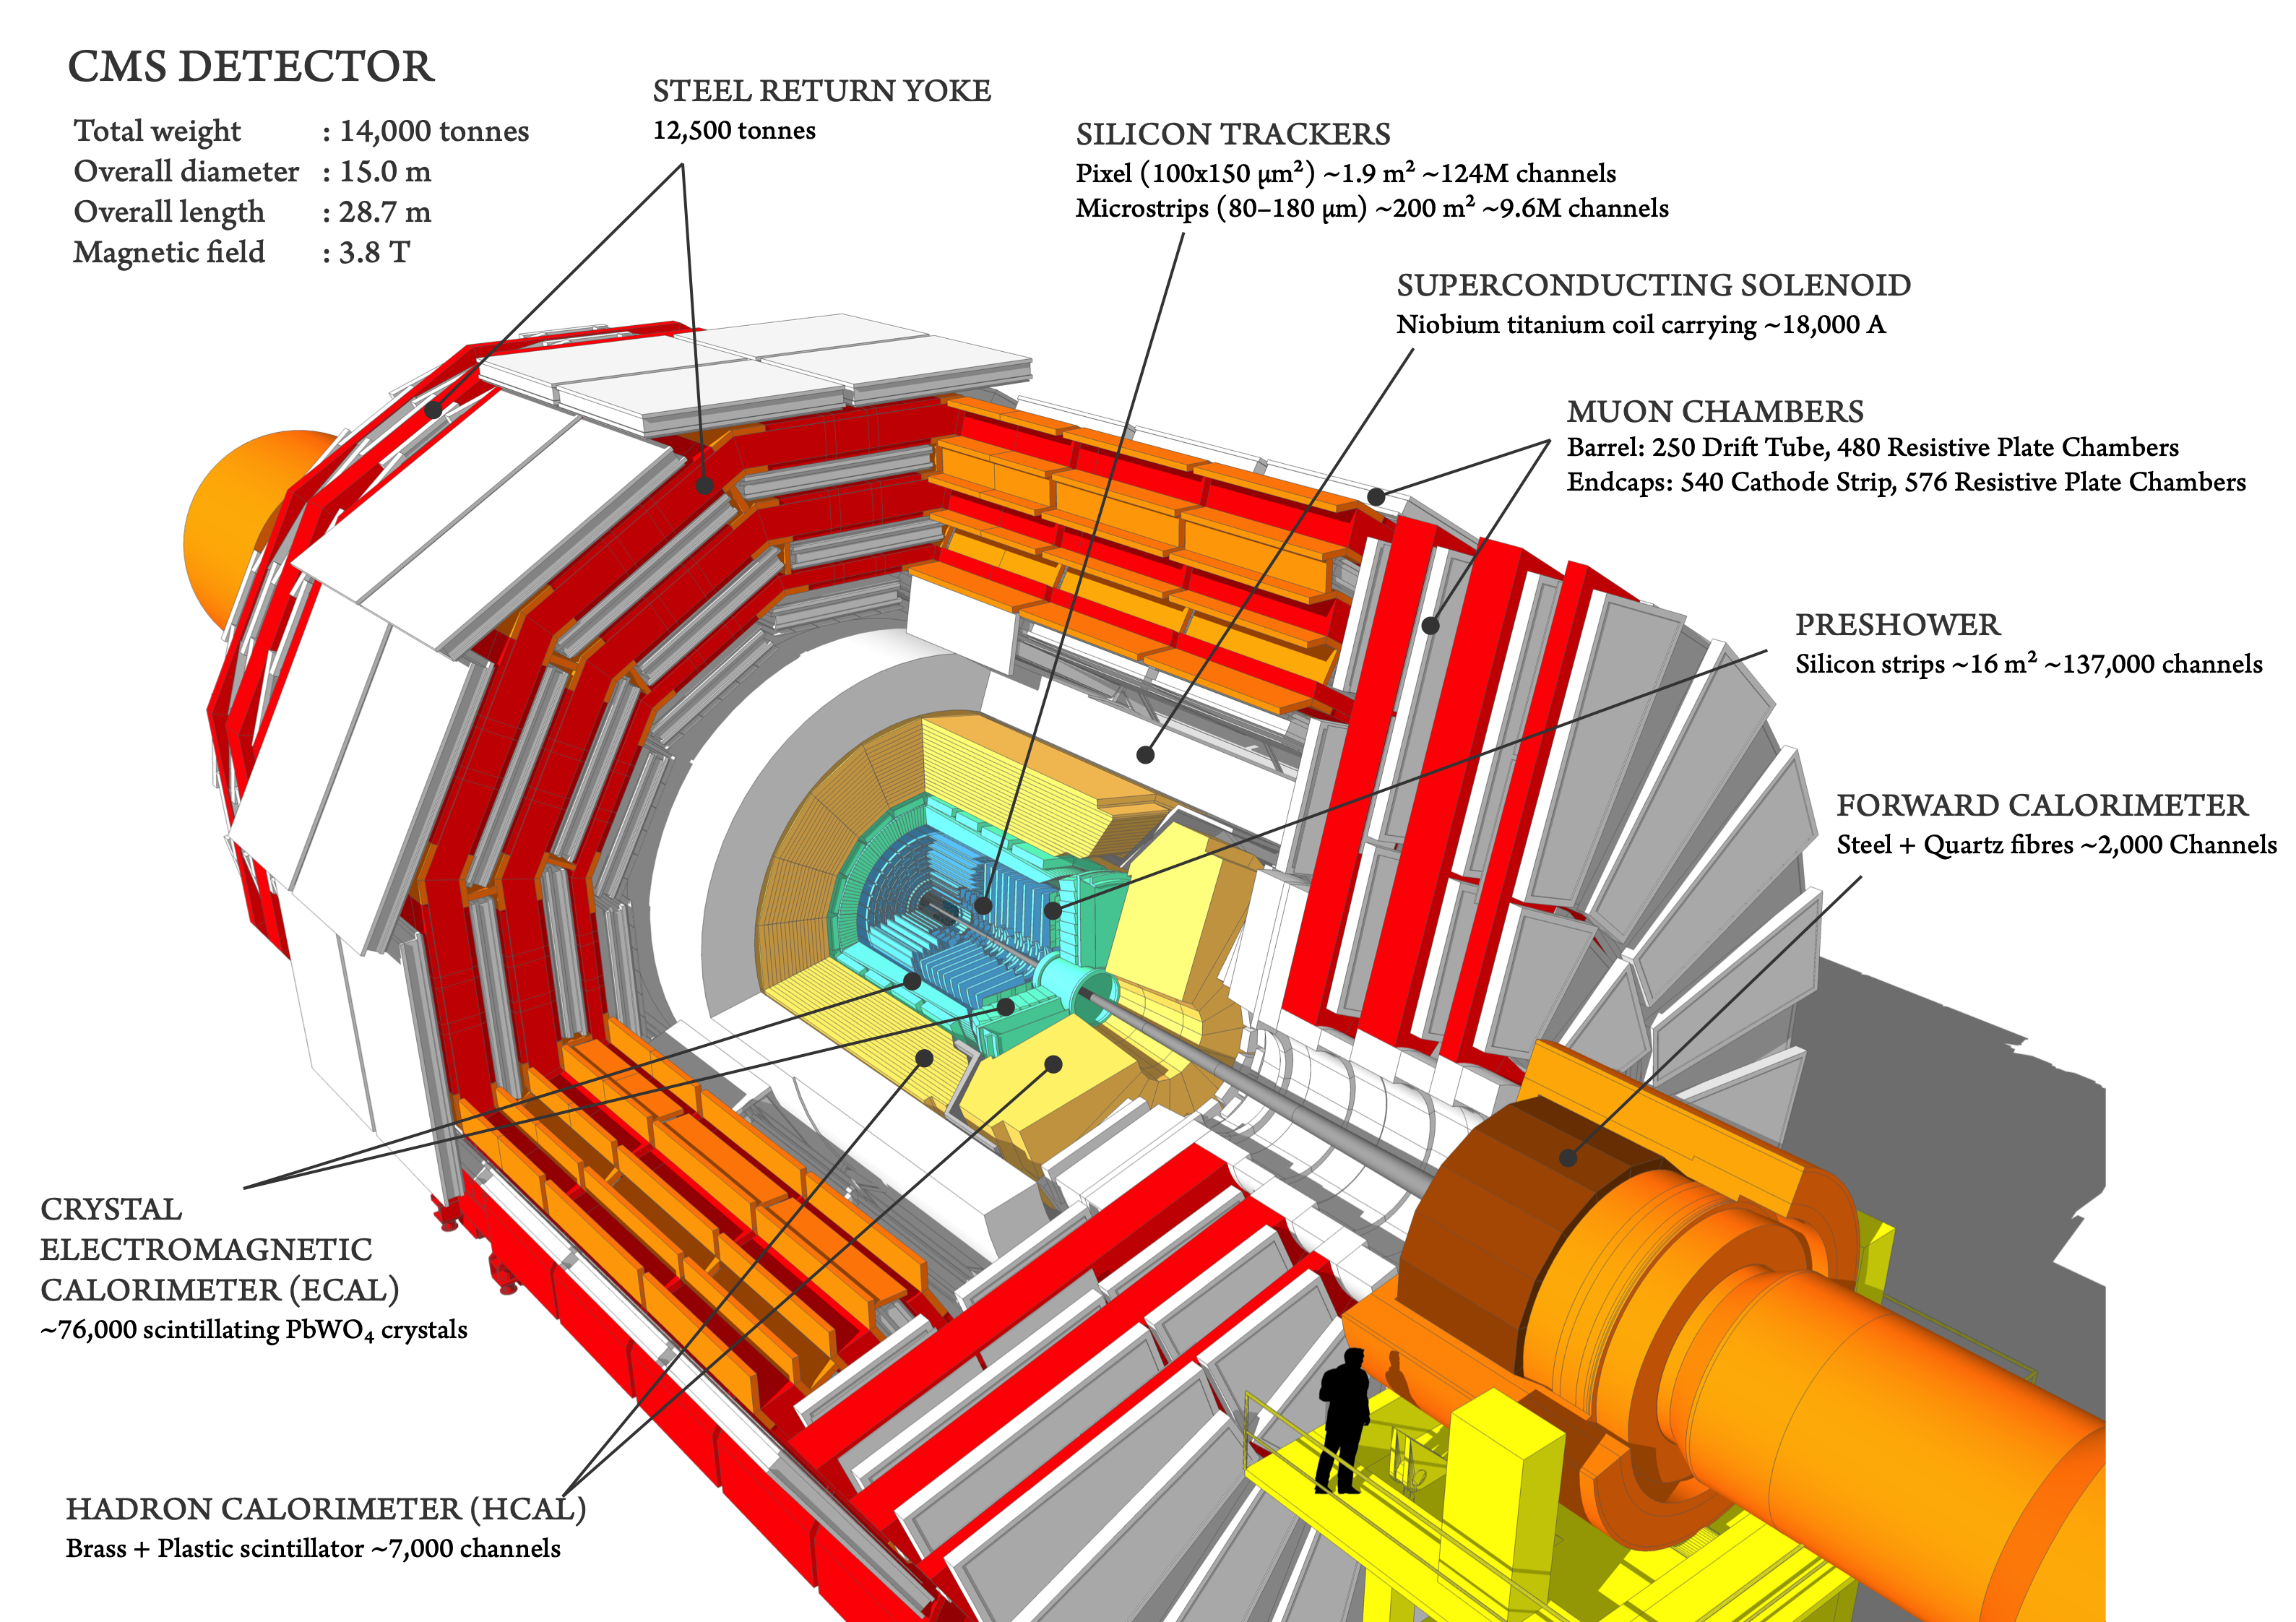
\includegraphics[height=9cm, width=13cm]{pictures/CMS_detector.png}
 \label{fig:1.5}
\end{figure}

CMS被设计为通用探测器,能够在LHC粒子加速器的质心能量0.9-13 TeV下研究质子碰撞的许多物理内容。CMS探测器围绕一个巨大的螺线管磁铁构建。它采用圆柱形超导电缆线圈的形式,产生4T的磁场,大约是地球磁场的100000倍。磁场被限制产生在12500吨重量的的探测器主体——钢轭内。CMS探测器的一个不同寻常的特点是,它不像大型强子对撞机实验中的其他巨型探测器那样在地下原位建造,而是在地面上建造,然后分15个部分被降到地下并重新组装。

CMS探测器包含用于测量光子、电子、$\mu$子和其他碰撞产物的能量和动量的子系统。最内层是硅基径迹探测器,被闪烁晶体电磁量能器所包裹,而闪烁晶体电磁量能器本身又被一个强子采样量能器包围。径迹探测器和量能器足够紧凑,可以安装在CMS螺线管内,该螺线管可产生3.8T的强大磁场。磁体外部是大型μ子探测器,它们位于磁铁的返回轭内。
	\chapter{大动量希格斯粒子和XWW共振态的物理和研究动机}
\label{chap2}
\fontsize{12bp}{14.4pt}

\section{希格斯粒子的产生和衰变}
在标准模型中,夸克、轻子、W、Z玻色子都通过希格斯机制被赋予质量。LHC以及下一代对撞机实验的重要目标之一就是研究测量希格斯粒子的相关性质,因此,对LHC上希格斯粒子的产生和衰变测量本身就是极为重要的一个任务。

本节除了讨论希格斯粒子的产生和衰变,还将讨论LHC上大动量希格斯粒子的物理特性和研究动机,并且指出我们感兴趣的$X\to WW$共振态搜寻的物理背景和动机(包括标准模型的希格斯粒子以及非标准模型的共振态)
\subsection{希格斯粒子的产生}
LHC上标准模型希格斯粒子的产生道如下\textbf{表\ref{table:2.1}}所示
\begin{table}[htbp]
    \caption{标准模型中希格斯粒子的产生道和相关参数\cite{Higgs_cross_sections}}\label{table:2.1}
    \centering
    \begin{tabular}{>{\centering\arraybackslash}p{2cm}%
    >{\centering\arraybackslash}p{7cm}%
    >{\centering\arraybackslash}p{2cm}%
    >{\centering\arraybackslash}p{2cm}}
    \toprule\toprule
    \textbf{产生道} & \textbf{产生方式} & \textbf{分支比} & \textbf{截面}\\
    \midrule
    ggF & 胶子通过b/top夸克圈聚合产生 & $\sim 87\%$ & \SI{48.5}{pb}\\
    VBF & W/Z矢量玻色子聚合产生 & $\sim7\%$ & \SI{3.78}{pb}\\
    WH & W/Z矢量玻色子与希格斯联合产生 & $\sim 4\%$ & \SI{1.37}{pb}\\
    ttH & 正反top夸克与希格斯联合产生 & $\sim1\%$ & \SI{0.51}{pb}\\
    bbH & 正反bottom夸克与希格斯联合产生 &  $\sim 1\%$ & \SI{0.49}{pb}\\
    tH & t,b,$q^\prime$与希格斯联合产生 & $\sim 0.1\%$ & \SI{0.09}{pb}\\
    \bottomrule\bottomrule
\end{tabular}
\end{table}\\
每个产生道都有独特的拓扑结构,对于其中的稀有道,尽管很难探测,却是研究超出标准模型物理的重要手段。

\subsection{希格斯粒子的衰变}
标准模型希格斯粒子的衰变道如下\textbf{表\ref{table:2.2}}所示,对于其中五个非稀有衰变道,有以下性质:
\begin{itemize}
    \item $\gamma\gamma$和$ZZ\to4\ell$道:高分辨度和高信噪比,常用来精确测量希格斯质量和微分散射截面。
    \item $WW$道:高分支比,但衰变末态的中微子导致低信噪比和低分辨度。
    \item $\tau\tau$和$bb$道:高分支比,低信噪比,用于直接探测希格斯粒子与费米子的耦合。
\end{itemize}
\begin{table}[htbp]
    \caption{标准模型中希格斯粒子的衰变道和相关参数\cite{Higgs_cross_sections}}\label{table:2.2}
    \centering
    \begin{tabular}{>{\centering\arraybackslash}p{2cm}%
    >{\centering\arraybackslash}p{7cm}%
    >{\centering\arraybackslash}p{2cm}%
    >{\centering\arraybackslash}p{2cm}}
    \toprule\toprule
    \textbf{衰变道} & \textbf{主要衰变方式(领头阶)} & \textbf{分支比} & \textbf{稀有衰变}\\
    \midrule
    $H\to bb$ & 直接衰变 & $\sim 58.1\%$ & 否\\
    $H\to WW$ & 直接衰变,一个在壳一个离壳 & $\sim 21.5\%$ & 否\\
    $H\to\tau\tau$ & 直接衰变 & $\sim 6.26\%$ & 否\\
    $H\to ZZ$ & 直接衰变 & $\sim2.64\%$ & 否\\
    $H\to \gamma\gamma$ & 通过W/t/b/$\tau$圈间接衰变 &  $\sim0.23\%$ & 否\\
    $H\to\mu\mu$ & 直接衰变 & $\sim 0.022\%$ & 是\\
    $H\to Z\gamma$ & 通过W/t/b/$\tau$圈间接衰变 & $\sim 0.154\%$ & 是\\
    $H\to cc$ & 直接衰变 & $\sim2.88\%$ & 是\\
    $H\to gg$ & 通过top/bottom圈间接衰变 & $\sim 8.18\%$ & 是\\
    \bottomrule\bottomrule
\end{tabular}
\end{table}

\section{大动量希格斯粒子的物理特性和研究动机}
对于大动量希格斯粒子的一个重要特征,就是原本在常规希格斯粒子衰变中分开的两个喷注,在大动量希格斯粒子衰变场景下,会合并成一个喷注,如\textbf{图\ref{fig:2.1}}所示,所以,对大动量希格斯粒子的标记和分析都存在很多和常规情况截然不同的地方。
\begin{figure}[H]
 \centering
 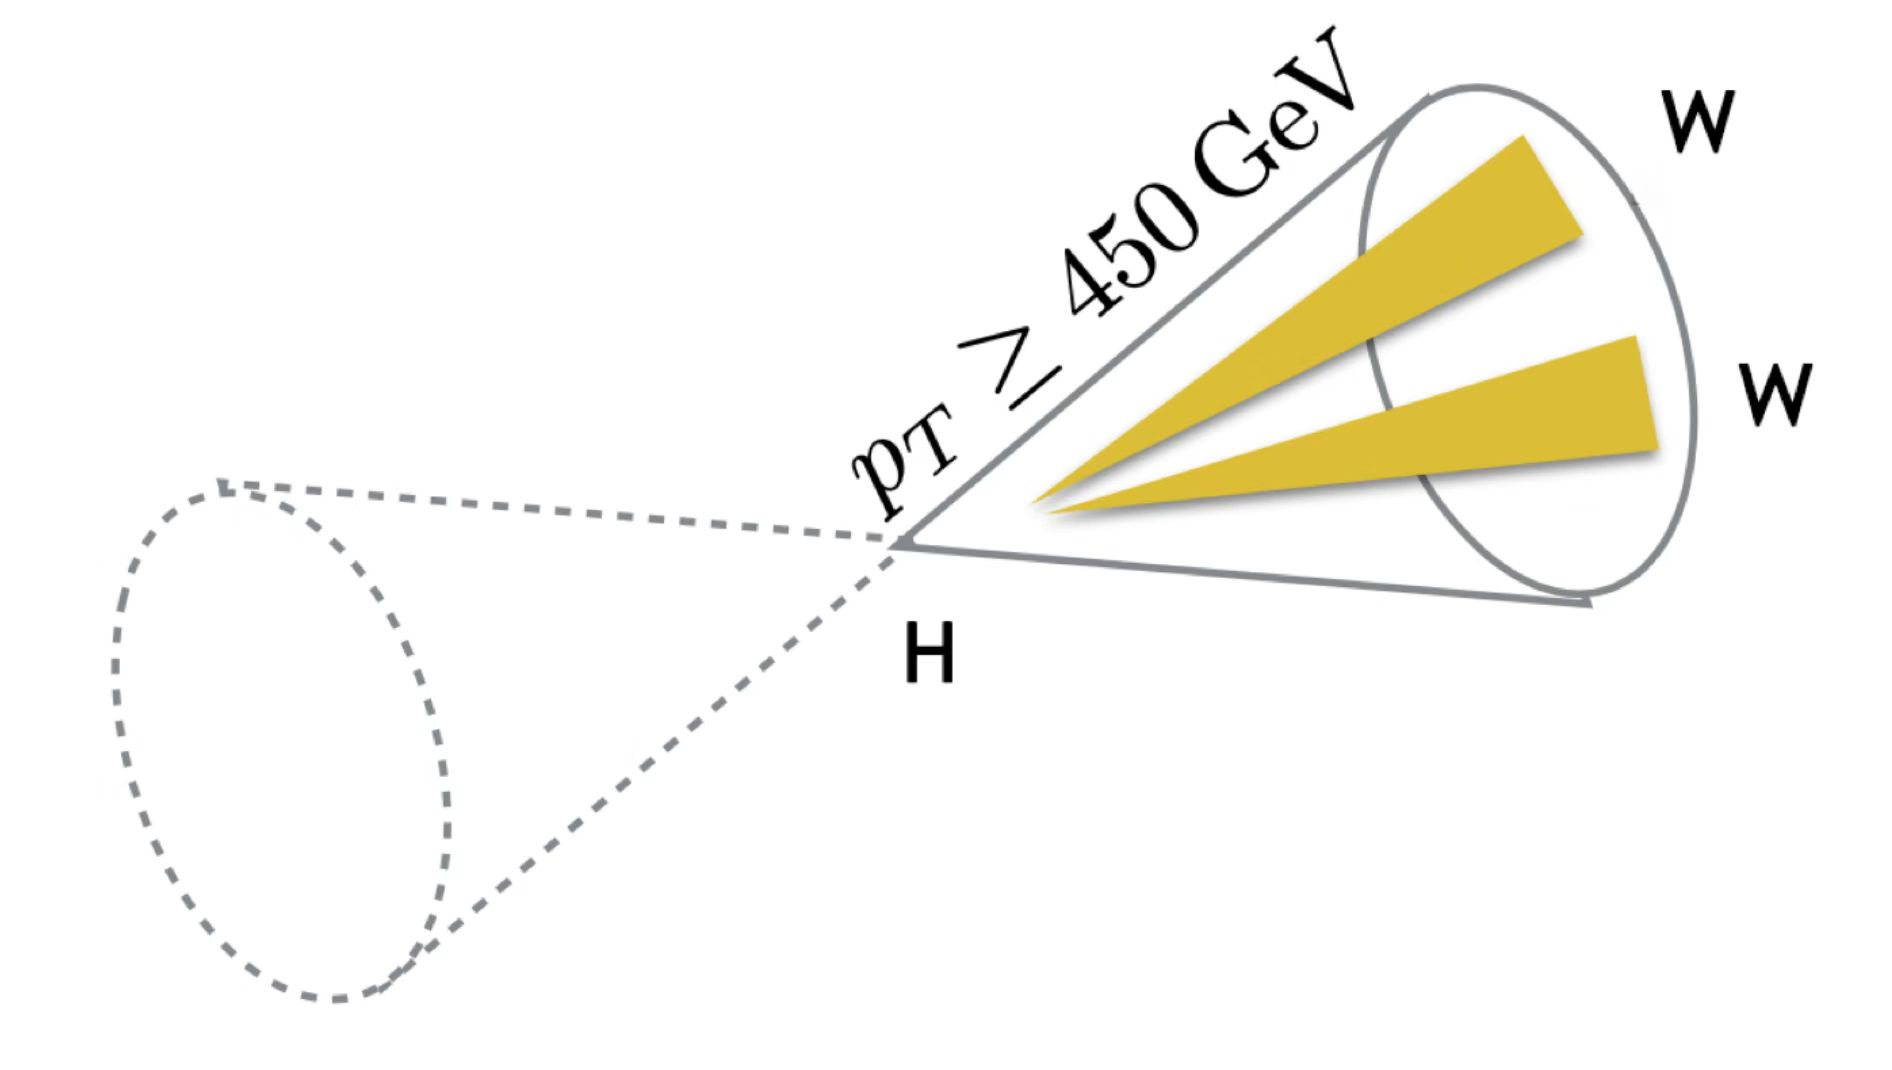
\includegraphics[height=6cm, width=10cm]{pictures/mergedjet.jpg}
  \caption{在动量足够大时,希格斯衰变产物会被重建到同一个喷注中}
 \label{fig:2.1}
\end{figure}

而对大动量希格斯粒子测量有如下物理动机:
\begin{enumerate}
    \item 可以提高标准模型希格斯测量的敏感度:在希格斯粒子$p_T>200$[GeV]的区域,$H\to bb$、$H\to\tau\tau$道还有未分辨出的喷注等待分析;在更高的$p_T$区域,$H\to ZZ/WW\to 4q$道也有同样的需求。
    \item 检验标准模型在大动量区域的高阶修正的正确性或者发现可能的新物理算符。
    \item 可以用作搜寻超出标准模型新物理的工具,包括:辐射子,Randall-Sundrum Bulk Graviton,复合希格斯粒子,新的矢量玻色子三重态,暗物质的探寻(2HDM)等。
\end{enumerate}

\begin{figure}[H]
 \centering
 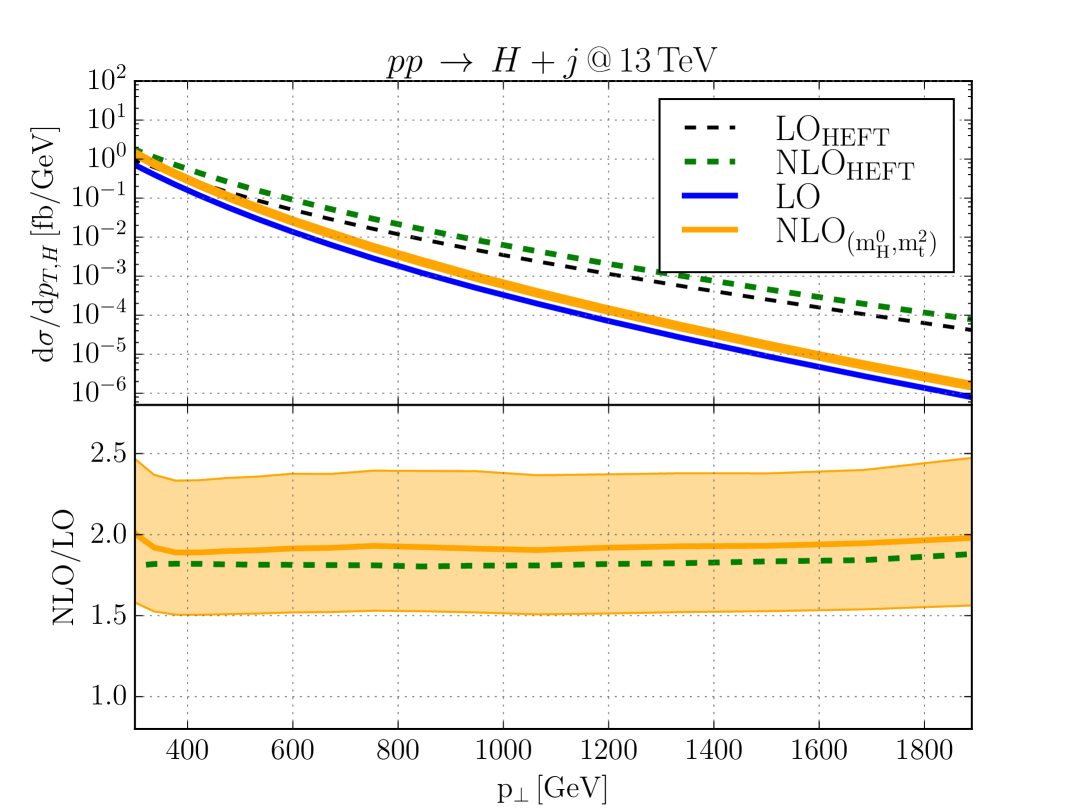
\includegraphics[height=8cm, width=11cm]{pictures/SM_NLO:LO.png}
  \caption{LHC上质心系能量为13TeV时希格斯玻色子的横向动量分布。上图显示标准模型和无穷大top质量有效场论(HEFT)中领头阶(LO)和次领头阶(NLO)的预测。下半部分显示了各自的NLO/LO校准比值。黄色边带表示由于尺度变化导致的标准模型结果的理论误差。\cite{Higgs_high_pt}}
 \label{fig:2.2}
\end{figure}

对于希格斯粒子的大动量区域,唯象上有以下结论\cite{Higgs_high_pt}:标准模型对希格斯粒子动量微分截面的高阶修正在高动量区十分稳定,次领头阶与领头阶的比值固定在一定值范围内(如上\textbf{图\ref{fig:2.1}}所示);而部分超标准模型理论\cite{Higgs_high_pt_BSM}的这一比值则会随动量增大而发生较大的增长(如下\textbf{图\ref{fig:2.2}}所示)。
\begin{figure}[H]
 \centering
 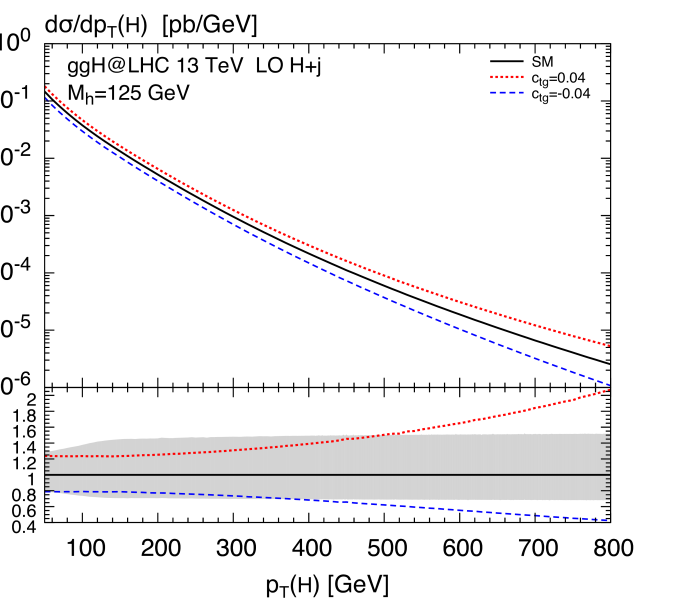
\includegraphics[height=9cm, width=9.8cm]{pictures/BSM_NLO:LO.png}
  \caption{超标准模型的chromomagnetic算符对实验允许范围内的希格斯玻色子谱分布。\cite{Higgs_high_pt_BSM}}
 \label{fig:2.3}
\end{figure}
所以对大动量区域希格斯粒子的搜寻和研究可以用来检验标准模型的精确性以及提供支持/反对新物理的证据。

除此之外,对大动量希格斯玻色子的搜寻还与其他新物理密切相关,比如测量希格斯粒子的属性与标准模型预言的偏差,有助于探索暗物质的性质和物质-反物质不对称性等谜团,因为高能标尺度的新物理无法在大型强子对撞机上直接观察到,但是,在量子场论中,高能标的新物理会间接产生虚粒子,从而导致产生的希格斯玻色子数量作为$p_T$的函数与标准模型会出现较大偏差。这也是我们研究大动量希格斯粒子的一个重要原因:间接地估计高能标尺度上的新物理敏感性。。

\section{$X\to WW$的物理背景及搜寻动机}
WW过程是LHC上第一批可观测到的双玻色子末态之一,而研究WW末态的最原始动机就是搜寻希格斯玻⾊⼦。当下,在CMS实验的RUN III即将开启运行和未来高通量LHC的展望下,我们研究WW共振态的目的就变成了对标准模型希格斯粒子的精确测量和搜寻超标准模型的新WW共振态。
\subsection{标准模型的$H\to WW$}
对于标准模型的$H\to WW$过程,衰变产物为一个质量在壳的$W$和一个质量离壳的$W^*$。所以也常写作$H\to WW^*$。
\begin{figure}[H]
 \centering
 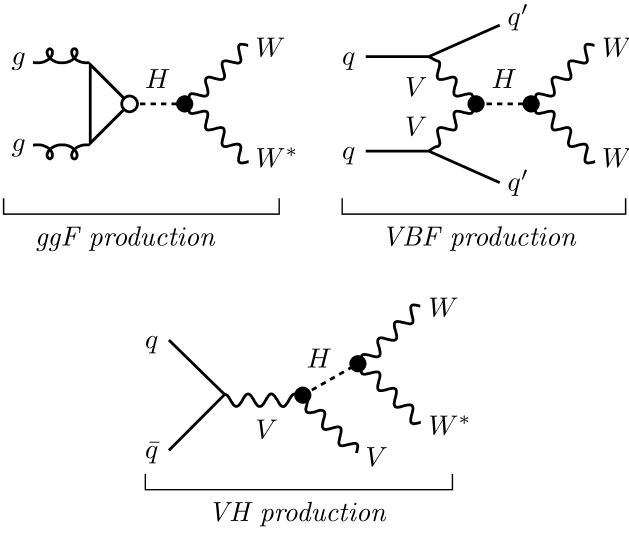
\includegraphics[height=8cm, width=10cm]{pictures/HWW_production.png}
  \caption{$H\to WW$的主要生产过程的领头阶费曼图:(a)通过夸克圈的ggF生产过程;(b)VBF生产过程,末态除了两个W玻色子之外还有两个夸克喷注;(c)VH联合产生,末态有三个玻色子}
 \label{fig:2.4}
\end{figure}
LHC上最多的$H\to WW$产生过程就是胶子聚合产生(ggF),如\textbf{图\ref{fig:2.4}左上}所示。初态胶子通过top夸克圈耦合成希格斯粒子,然后希格斯粒子继续衰变成一对W玻色子。次多产生模式是矢量玻色子聚合产生(VBF),如\textbf{图\ref{fig:2.4}右上}所示,其生产截面大约比ggF小一个数量级。两个初态夸克辐射出W或Z玻色子,然后W或Z玻色子聚合成希格斯粒子,并进一步衰变成一对W玻色子。但VBF末态会生成两个喷注加一对W玻色子,而ggF只会生成一对W玻色子。

$H\to WW^*$的主要本底来自于标准模型下的非共振WW生产道连续谱。在LHC上,WW生产过程由$q\bar{q}$湮灭过程主导\cite{john-alison},如\textbf{图\ref{fig:2.5}}所示:左边和中间分别是$qq^\prime\to WW$过程的t通道图、s通道图,其中s通道过程对于$WWZ$和$WW\gamma$的三玻色子耦合顶点十分敏感。次领头阶的WW本底还有如右边所示的胶子聚合(ggF)生成WW的box图,尽管是次领头阶图,但这个过程被LHC上的高亮度胶子产物增强,从而对非共振态WW的产生贡献也不可忽视。
\begin{figure}[H]
 \centering
 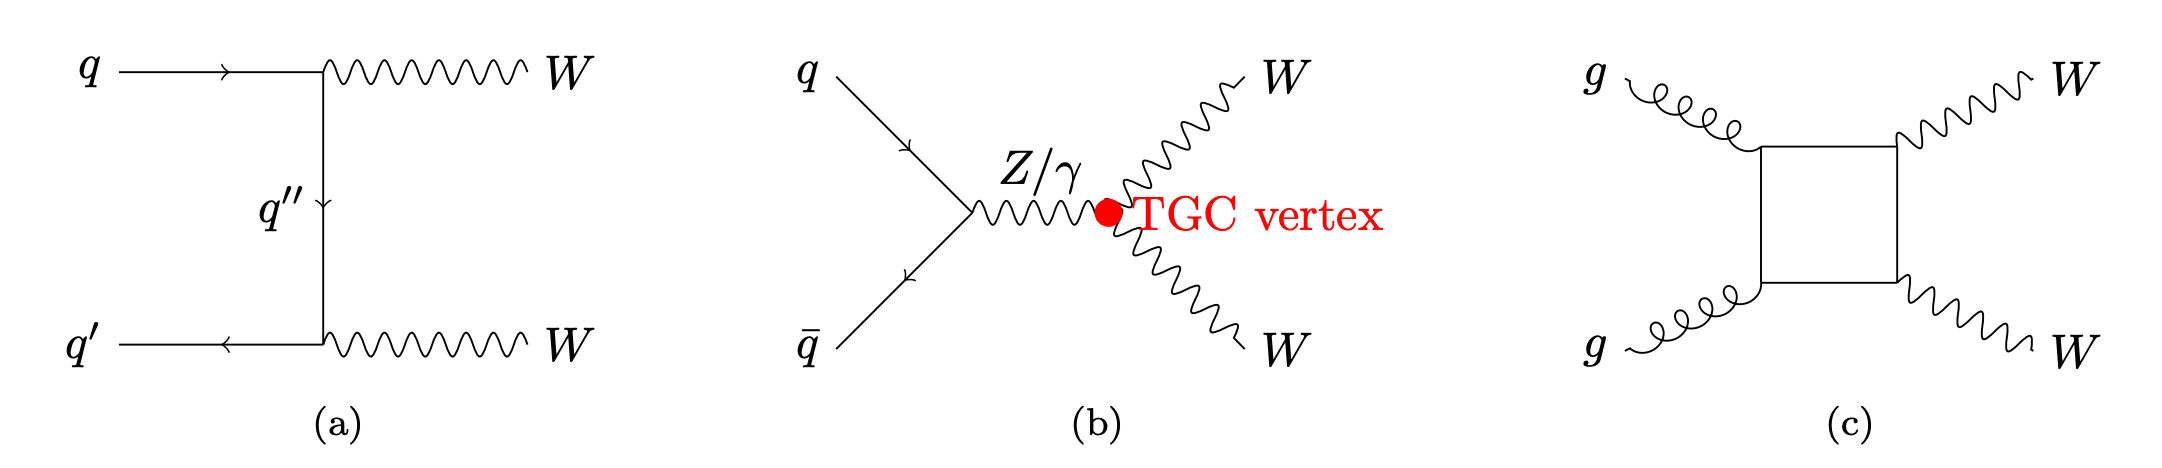
\includegraphics[height=4cm, width=16cm]{pictures/WW_bkg.png}
  \caption{标准模型非共振态$WW$的主要产生过程\cite{john-alison}:(a)$qq^\prime\to WW$的t通道图;(b)$qq^\prime\to WW$的s通道图,有一个三规范玻色子耦合顶点(TGC);(c)$gg\to WW$的box图,贡献被LHC的高亮度胶子抬高。}
 \label{fig:2.5}
\end{figure}

在标准模型框架下,研究双玻色子产生提供了在TeV尺度检验标准模型电弱理论的机会。WW过程就是其中重要的一个例子。除了$H\to WW$产生之外之外,WW产生过程还对三玻色子耦合顶点十分敏感(如\textbf{图\ref{fig:2.5}(b)}所示),从而提供了检验标准模型规范对称性(关于三玻色子耦合限制)的重要机会。通过对WW产生过程的三玻色子耦合的精确测量,我们有机会探寻到包含规范玻色子的新物理现象。(见\ref{sec:2.3.2}节)

\subsection{超标准模型的$X\to WW$}\label{sec:2.3.2}
对于标准模型的$H\to WW$共振态和更重质量的$WW$共振态X,它们的喷注重建也存在区别,如下图所示,重质量的XWW共振态会产生大动量的W玻色子从而导致每个W衰变的两夸克喷注被重建在同一个W喷注里。
\begin{figure}[H]
 \centering
 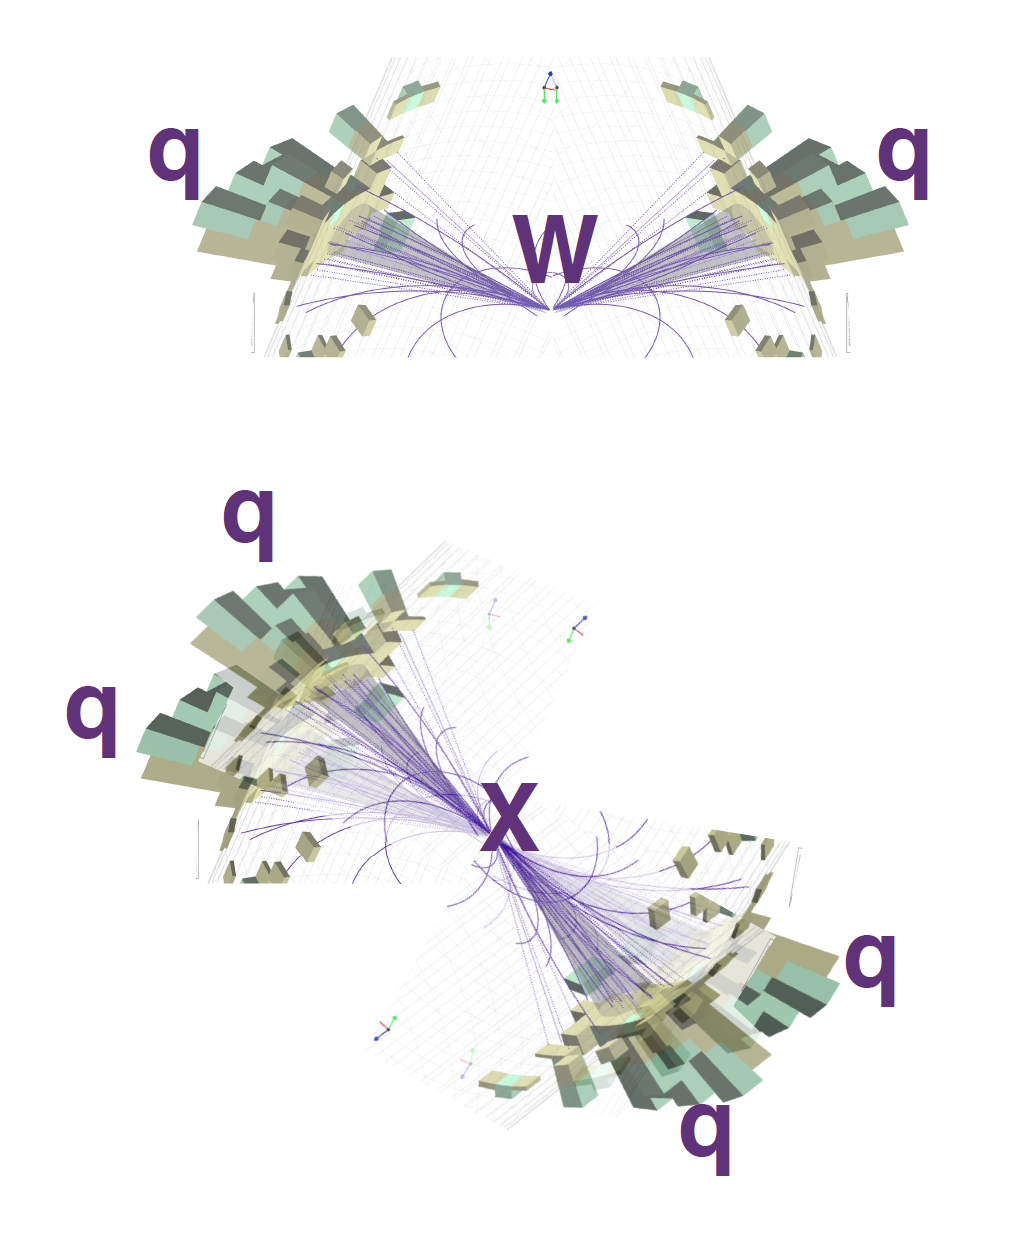
\includegraphics[height=13cm, width=10cm]{pictures/massiveXWW.png}
  \caption{低$p_T$的W玻色子衰变出的两个夸克会被重建为两个喷注,重质量的XWW共振态会产生两个大动量的W玻色子从而导致每个W衰变的两夸克被重建合并为一个喷注。\cite{Boosting_the_Higgs_boson}}
 \label{fig:2.6}
\end{figure}

在这样的物理背景下,对超标准模型的XWW共振态搜寻有助于探寻$V_{kk}$等重质量新物理粒子,如下\textbf{图\ref{fig:2.7}}所示
\begin{figure}[H]
 \centering
 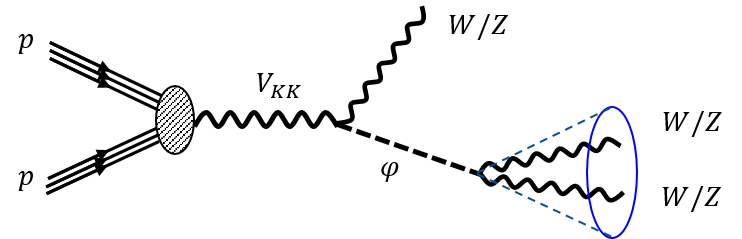
\includegraphics[height=5cm, width=16cm]{pictures/Vkk.png}
  \caption{可考虑的超出标准模型物理过程,基于扭曲的额外维RS模型的扩展。$V_{kk}$表示$W/Z$的Kaluza-Klein(KK)模式,并且对应于较重的母粒子。$\phi$表示标量粒子,被认为是标准模型中的EW规范玻色子。两个$W/Z$粒子周围来自$\phi$衰变的圆锥体表明它们是高度准直的。\cite{Detecting_a_Boosted_Diboson_Resonance}}
 \label{fig:2.7}
\end{figure}

除了对重质量新物理粒子的搜寻,$X\to WW$共振态还可以用来研究非标准模型质量希格斯粒子的衰变分支比关系,如\textbf{图\ref{fig:2.8}}展示了希格斯衰变分支比作为希格斯质量的函数。可以看到双W衰变道在很大的质量范围内都是是最大分支比。特别是当$M_H>130$[GeV]时,就主要是HWW衰变了。在$2m_W<M_H<2m_Z$时,是$H\to WW$分支比非常显著的区间。
\begin{figure}[H]
 \centering
 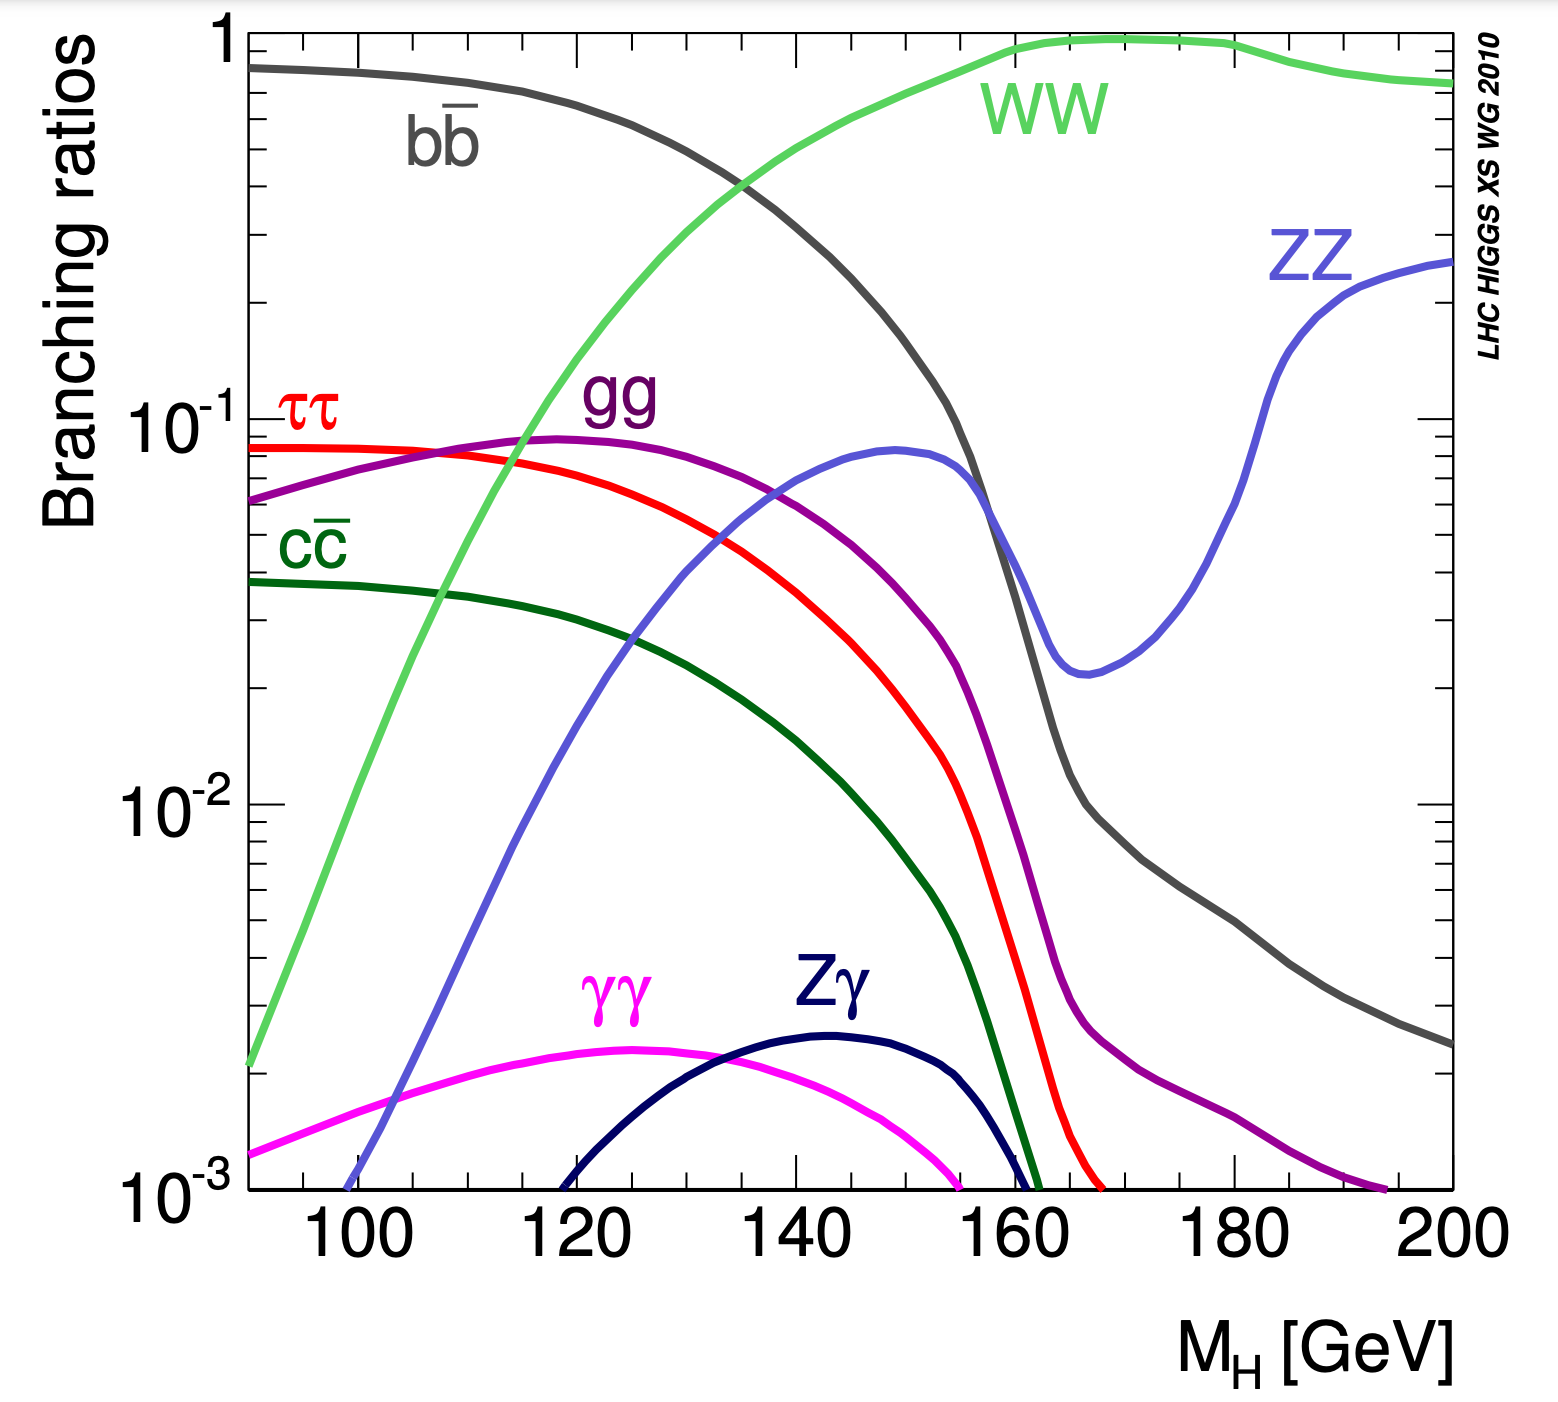
\includegraphics[height=8cm, width=10cm]{pictures/XS-MH.png}
  \caption{不同质量希格斯粒子的衰变分支比}
 \label{fig:2.8}
\end{figure}
因为我们知道$H\to WW$产⽣的速率由希格斯到WW的分⽀⽐决定,所以如果测量得到的$H\to WW$数目与标准模型预言有较大偏差,就暗示着有可能存在着非标准模型质量的伴生/复合希格斯粒子。

如下\textbf{图\ref{fig:2.9}}所示,展示了一种可能的复合希格斯粒子的新物理模型\cite{Boosting_the_Higgs_boson}
\begin{figure}[H]
 \centering
 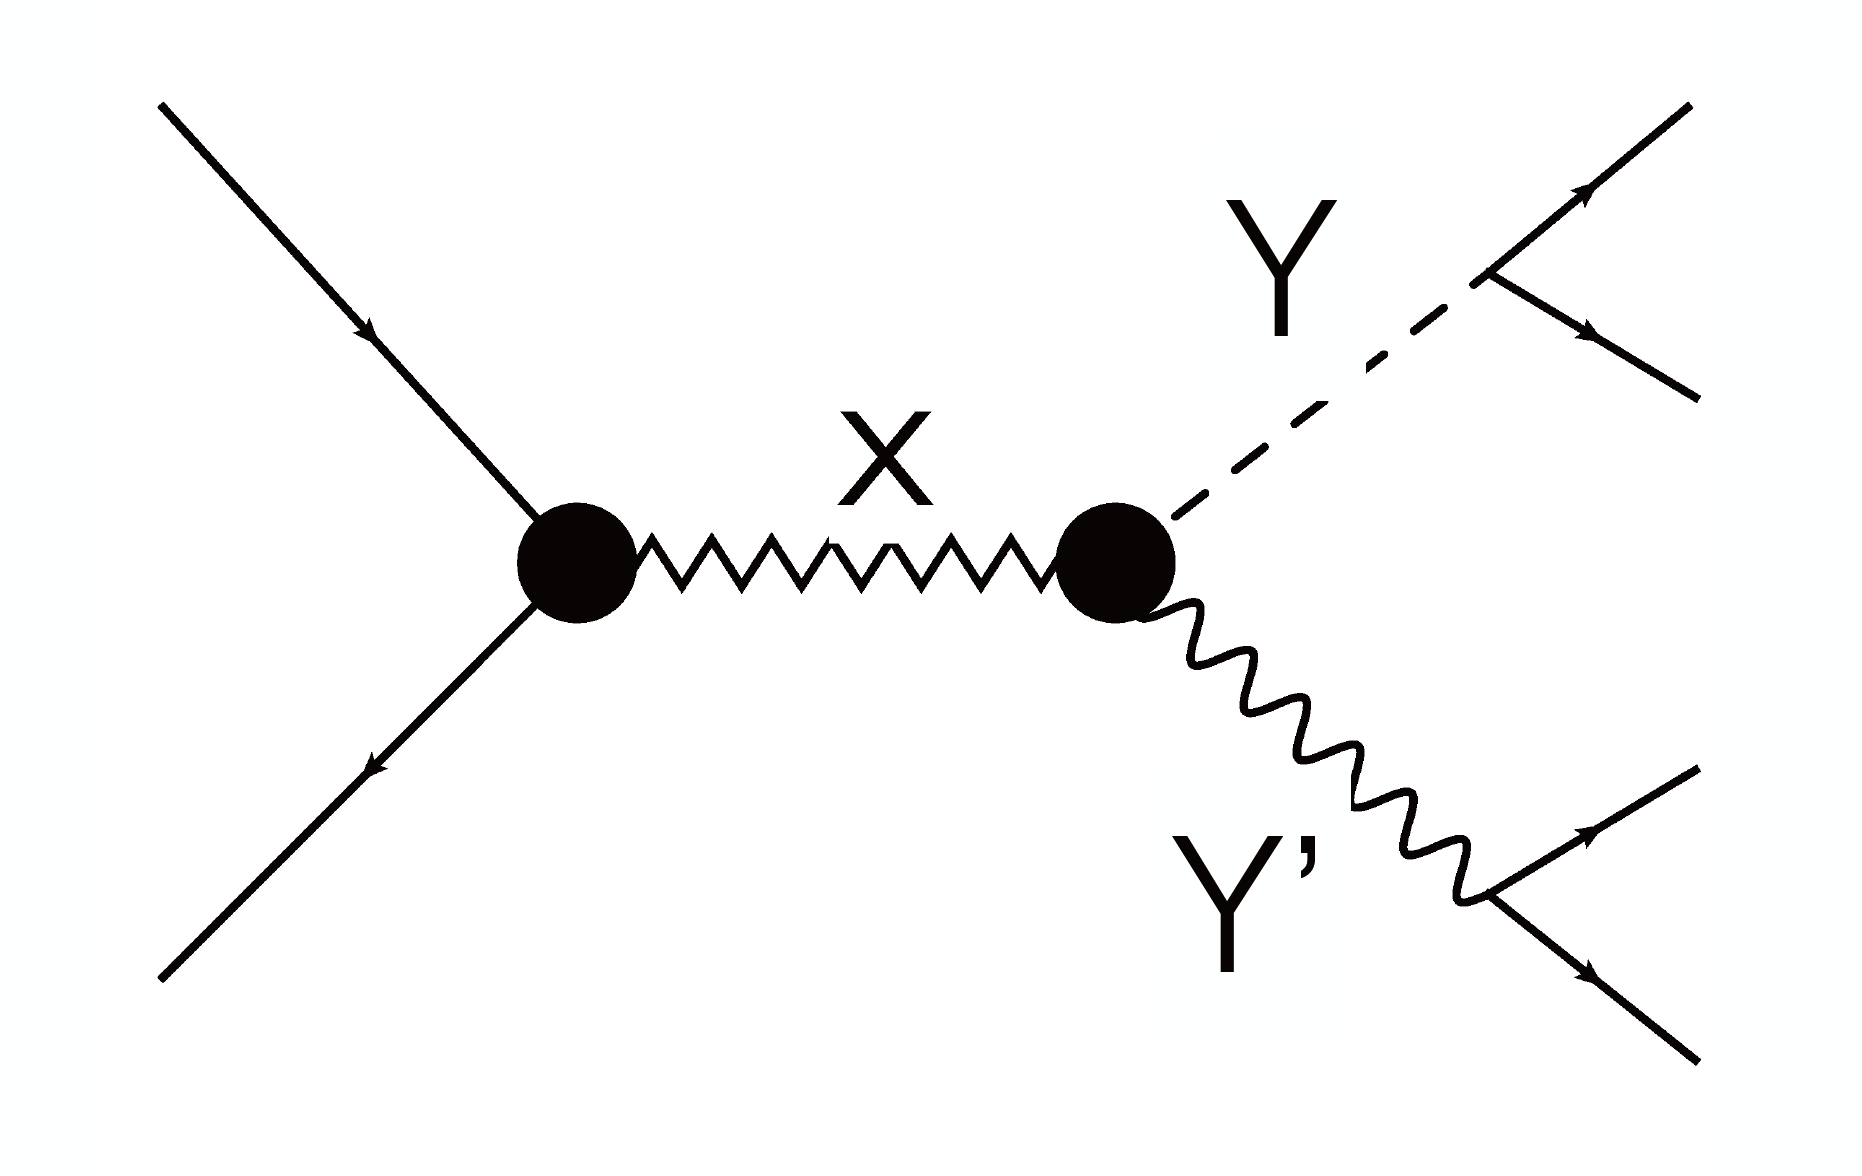
\includegraphics[height=6cm, width=10cm]{pictures/diboson_resonance_X.png}
  \caption{$X$代表TeV能量尺度的新物理粒子,$Y/Y^\prime$是$W/Z/H$玻色子。}
 \label{fig:2.9}
\end{figure}
对$X\to WW$共振态的搜寻,可以提供类似上图新物理过程的证据,发现可能的额外维度拉格朗日项、复合的希格斯粒子以及扩展的规范对称性(更多种类的$Z/W$玻色子)。

	\chapter{CMS实验的重建与标记技术介绍}
\label{chap3}
\fontsize{12bp}{14.4pt}
\section{重建事例时缓解顶点堆积的puppi算法}
\subsection{顶点堆积(pile-up)}
事例堆积(pile-up)是指:大型强子对撞机(以及所有粒子物理加速器)上的质子流是一束一束的,而不是连续的。每次当一个质子流中的一束遭遇另一个质子流中的一束时,会有多个质子彼此相互作用。通常,只有其中的硬散射才能产生我们感兴趣的粒子,但在两束质子遭遇时一般只有小于等于一个相互作用顶点是“硬散射”。尽管如此,硬散射以外的相互作用仍然会大量发生,并且每个相互作用都会产生一些新粒子。这就是我们所说的堆积(pile-up)。(另一种说法是“多重相互作用”)

堆积对于我们重建事例会造成困难,一个通俗的理解方式就是烟花,如下\textbf{图\ref{fig:3.1}}所示
\begin{figure}[H]
 \centering
 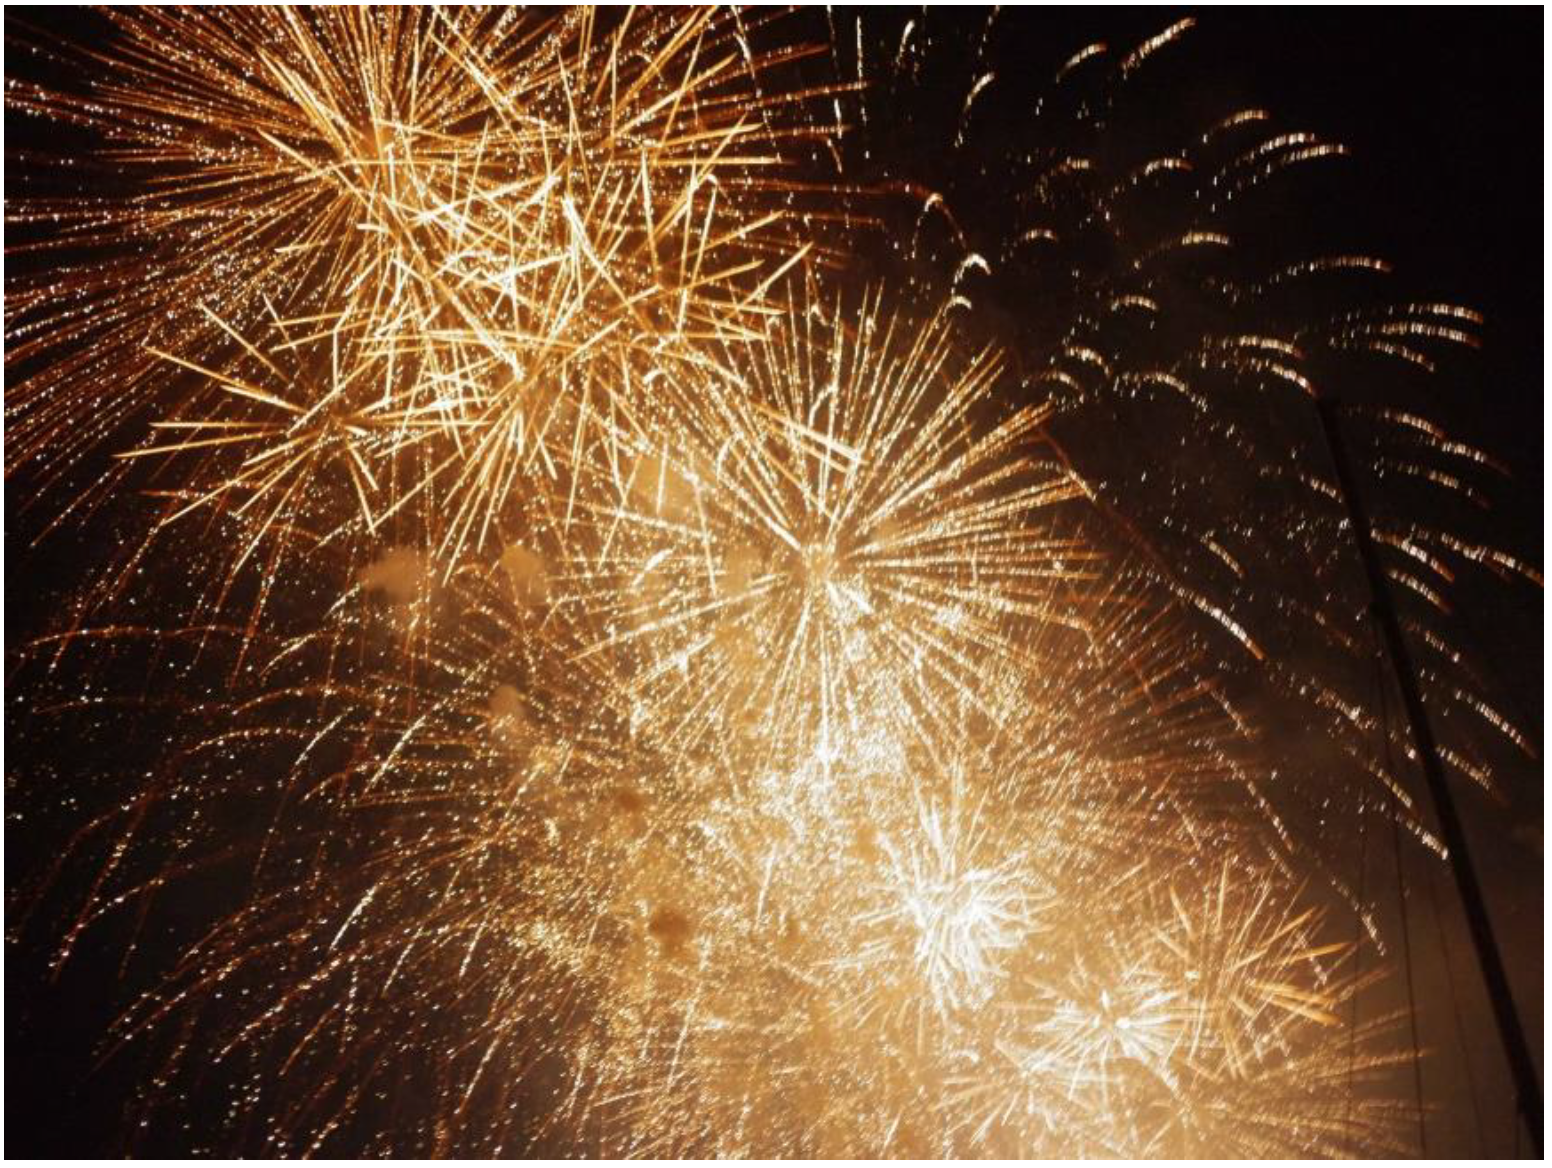
\includegraphics[height=8cm, width=10cm]{pictures/firework.png}
 \caption{把烟花绽放顶点比作事例顶点,烟花出射轨迹比作事例出射粒子/喷注}
 \label{fig:2.1}
\end{figure}
我们在按照出射轨迹重建“烟花”顶点时,还会受到周围其他“烟花”顶点出射轨迹的影响,从而对我们重建感兴趣的“烟花”顶点造成很大困难。

\subsection{puppi算法}
现在CMS实验中使用puppi算法来解决堆积困难,其全称是Pile-Up Per Particle Identification\cite{Pileup_Per_Particle_Identification},以下是对该算法的介绍。

对于一个事例中的每个粒子i,我们可以定义一个变量$\alpha_i$满足
\begin{equation}\label{define_alpha_i}
    \alpha_{i}=\log\sum_{\begin{subarray}{c}j\in{\text{Event}}\end{subarray}}\frac{p_{Tj}}{R_{ij}}\times\Theta(R_{\text{min}}\leq\Delta R_{ij}\leq R_{0})
\end{equation}
这里$\Theta(R_{\text{min}}\leq\Delta R_{ij}\leq R_{0})\equiv\Theta(\Delta R_{ij}-R_{\text{min}})\times\Theta(R_{0}-\Delta R_{ij})$,$\Theta$是阶跃函数,$\Delta R_{ij}$是粒子i和j在$\eta - \phi$空间的距离,$p_{Tj}$是粒子j的横向动量(单位为[GeV]),$R_0$定义了每个粒子i附近的圆锥所以只有在圆锥内的粒子才会参与$\alpha_i$的计算。除此之外,离粒子i距离小于$R_{min}$的粒子也会被从求和中舍弃,$R_{min}$作为粒子i的共线分裂调整器。通常取$R_0=0.3$,$R_{min}=0.02$。

在Particle-Flow中,我们可以把所有粒子候选者分为三类:中性粒子;来自领头顶点的带电强子;来自堆积顶点的带电强子。这样我们可以把\eqref{define_alpha_i}中的求和分解为
\begin{equation}
    \sum_{j\in\rm Event}=\sum_{j\in\rm Ch,PU}+\sum_{j\in\rm Ch,LV}+\sum_{j\in\rm Neutral}
\end{equation}
因此,我们可以使用来自领头顶点的带电粒子作为来自领头顶点的所有粒子的代理。

当带电粒子径迹信息可用时,我们可以计算出粒子i与所有来自领头顶点的带电粒子的关系如下
\begin{equation}
    \alpha_{i}^C=\log\sum_{\begin{subarray}{c}j\in{\text{Ch,LV}}\end{subarray}}\frac{p_{Tj}}{R_{ij}}\times\Theta(R_{\text{min}}\leq\Delta R_{ij}\leq R_{0})
\end{equation}

\begin{figure}[H]
 \centering\label{fig:3.2}
 \caption{$p_{T}>1~{}\mathrm{GeV}$时,领头顶点和堆积顶点出射粒子的$\alpha^C_i$变量分布\cite{Pileup_Per_Particle_Identification}}
 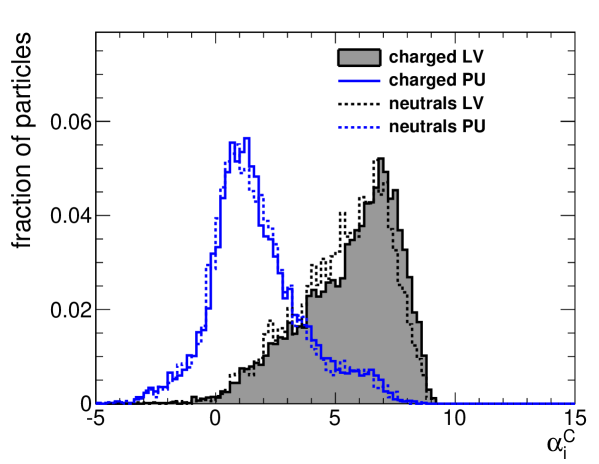
\includegraphics[height=8cm, width=10cm]{pictures/puppi_aC.png}
\end{figure}

当带电粒子径迹信息不可用时,我们只能计算出粒子i与来自领头顶点的所有粒子的关系如下
\begin{equation}
    \alpha^F_{i}\equiv\alpha_{i}=\log\sum_{\begin{subarray}{c}j\in{\text{Event}}\end{subarray}}\frac{p_{Tj}}{R_{ij}}\times\Theta(R_{\text{min}}\leq\Delta R_{ij}\leq R_{0})
\end{equation}
同时,我们假设总和中的所有粒子都来自领头顶点,虽然有来自堆积顶点的噪音贡献,但相对于领头顶点粒子的贡献会被分子上的$p_{Tj}$所抑制。这样的话算法就仍可以为没有径迹信息的区域分配权重。

\begin{figure}[H]
 \centering\label{fig:3.3}
 \caption{$p_{T}>1~{}\mathrm{GeV}$时,领头顶点和堆积顶点出射粒子的$\alpha^F_i$变量分布\cite{Pileup_Per_Particle_Identification}}
 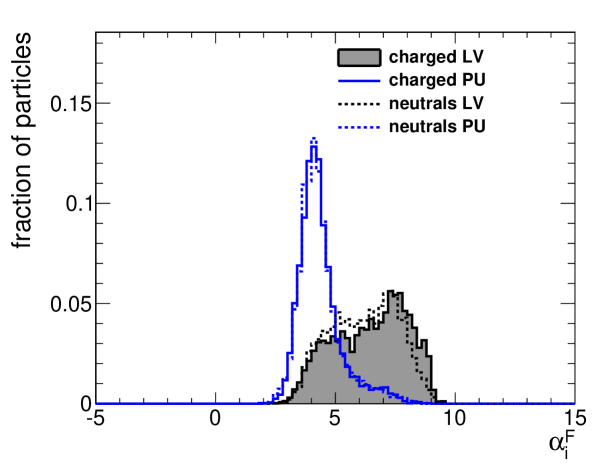
\includegraphics[height=8cm, width=10cm]{pictures/puppi_aF.png}
\end{figure}

利用带电粒子径迹信息可以获得一个好处:对于带电粒子,我们可以利用径迹信息知道其是否来自堆积顶点,从而可以计算$\alpha^F_i$和$\alpha_i^C$;对于中性粒子,我们在重建水平无法知道其是否来自堆积顶点,所以我们可以用带电粒子的$\alpha^F_i$和$\alpha_i^C$估计中性粒子的对应分布(这暗示了带电粒子和中性粒子具有相同分布,这一点可以从\textbf{图\ref{fig:2.2}}和从\textbf{图\ref{fig:2.3}}中看出。

现在,我们用中位数和标准差表征领头顶点和堆积顶点的$\alpha^F_i$和$\alpha_i^C$:
\begin{equation}
    \bar{\alpha}^{F}_{\text{PU}}\text{median}\{\alpha^{F}_{i\in\text{Ch,PU}}\},\hskip 40.00006pt\sigma^{F}_{\text{PU}}=\text{RMS}\{\alpha^{F}_{i\in\text{Ch,PU}}\}
\end{equation}
\begin{equation}
    \bar{\alpha}^{C}_{\text{PU}}\text{median}\{\alpha^{F}_{i\in\text{Ch,PU}}\},\hskip 40.00006pt\sigma^{F}_{\text{PU}}=\text{RMS}\{\alpha^{F}_{i\in\text{Ch,PU}}\}
\end{equation}

接着为了区分来自领头顶点和来自堆积顶点的粒子,我们引入了一个变量以区分这两类,并使用它来计算每个粒子的权重。该变量如下
\begin{equation}\label{eq:chi2}
    \chi_{i}^{2}=\Theta(\alpha_{i}-\bar{\alpha}_{\text{PU}})\times\frac{(\alpha_{i}-\bar{\alpha}_{\text{PU}})^{2}}{\sigma_{\text{PU}}^{2}}
\end{equation}
这里$\Theta$是阶跃函数,$\chi^2_i$用来度量$\alpha_i$与中位数$\bar{\alpha}_{\text{PU}})$的偏离程度。

然后是对粒子权重的定义:对于领头顶点粒子,理想权重是1,对于堆积顶点粒子理想权重是0。在实际中,为了在有限信息下估计一个粒子有多大可能来自堆积顶点,权重可以是介于0和1之间的任意值。我们把权重记为$w_i$,如下计算:
\begin{equation}\label{eq:weight}
    w_{i}\equiv F_{\chi^{2},\text{NDF}=1}(\chi_{i}^{2}),
\end{equation}
这里$F_{\chi^2}$是变量$\chi^2$的累积分布函数。

这样我们就知道,对于任何高于中位数的$\alpha_i$,$chi^2_i$都会对应于一个介于0和1之间的权重,并被认为可能来自于领头顶点;反之则对应权重为0的情况,并被认为来自于堆积顶点。

puppi算法在CMS实验上的效果如下\textbf{图\ref{fig:2.4}}所示,可以看到在堆积顶点数目上升时,重建顶点是领头顶点的纯度依然非常稳定接近于1
\begin{figure}[H]
 \centering
 \caption{puppi算法效果\cite{pileup-performance}}
 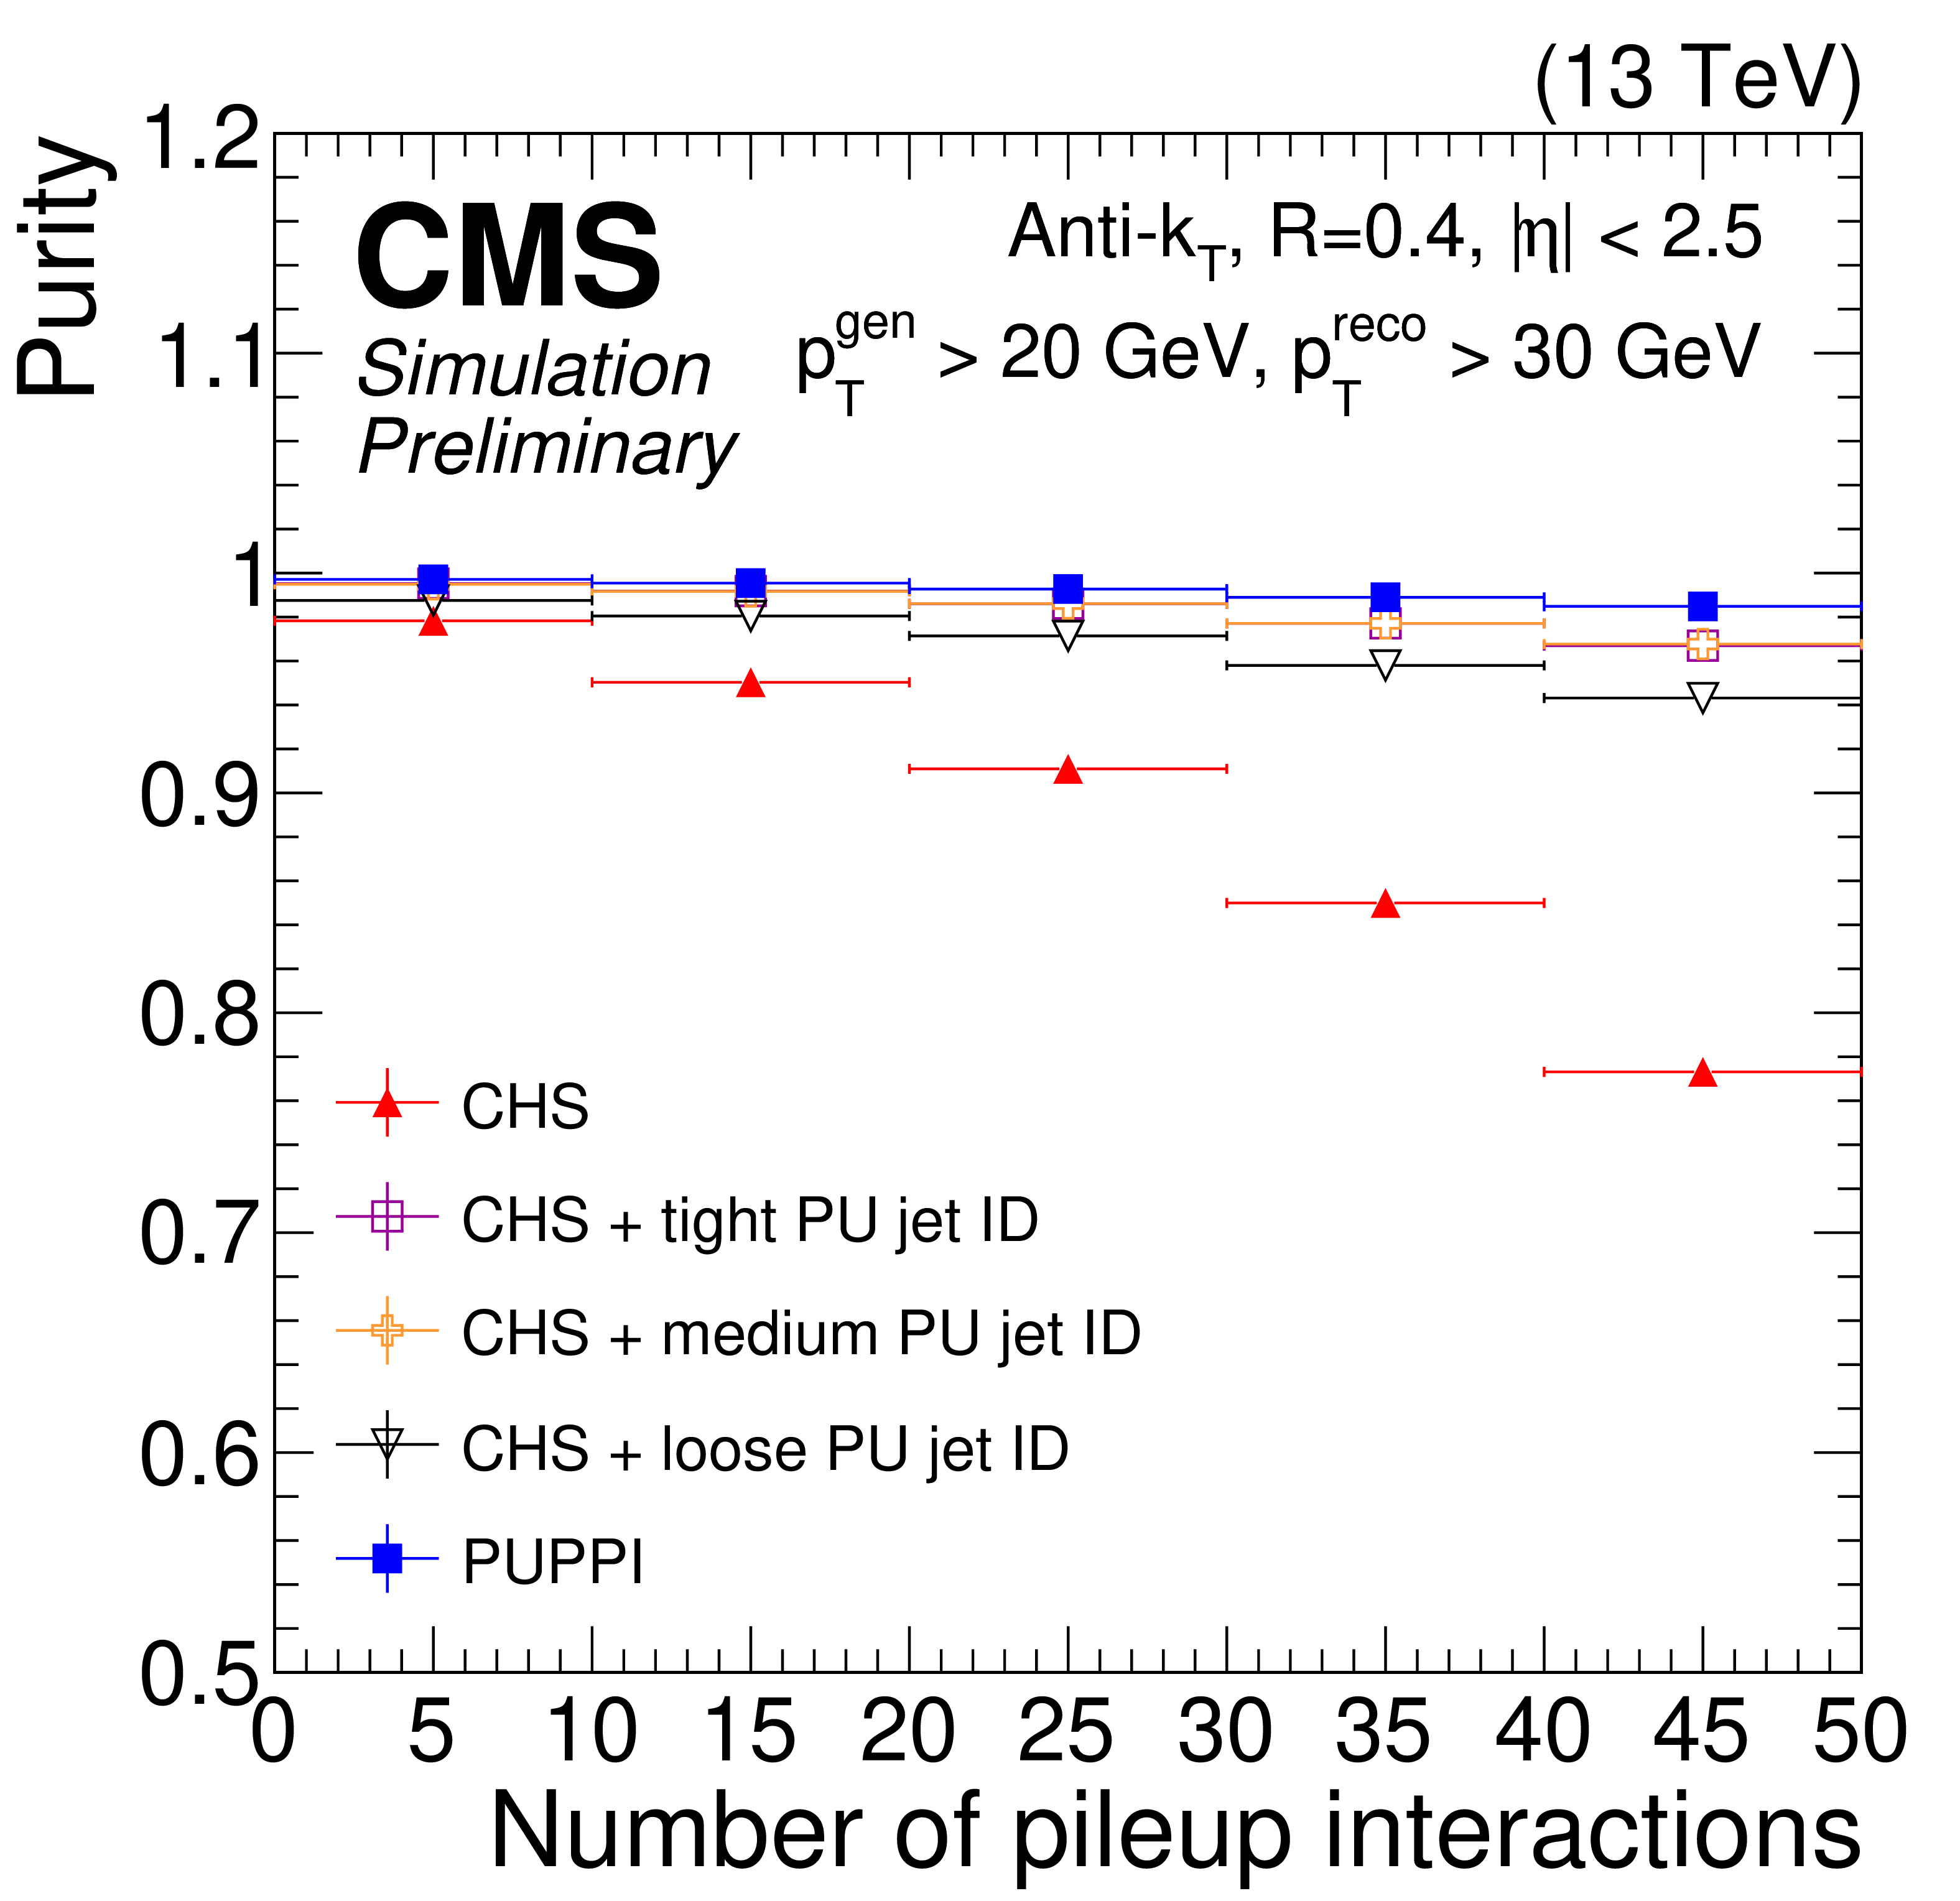
\includegraphics[height=9cm, width=10cm]{pictures/puppi_performance.png}
 \label{fig:3.4}
\end{figure}

至此,我们可以总结puppi算法流程如下:
\begin{enumerate}
    \item 计算事例中所有带电粒子的$\alpha^F_i$和$\alpha^C_i$以及对应的中位数和标准差。
    \item 所有来自堆积顶点的带电粒子权重都设为0,所有来自领头顶点的带电粒子权重都设为1。
    \item 然后使用方程\eqref{eq:chi2}和方程\eqref{eq:weight}来计算剩余粒子的权重。
    \item 所有粒子的四动量都进行重新加权:$p_i^\mu\to w_ip_i^\mu$。
    \item 权重或重加权动量小于一定阈值的粒子则被舍弃:$w_i<w_{cut}$或$p_{Ti}<p_{T,cut}$。
    \item 剩余被重加权粒子的集合则被当作是堆积修正了的事例。
\end{enumerate}

\section{重建喷注的Anti-$k_T$算法}
Jet 聚类算法是用于分析强子碰撞数据的主要工具之一,下面我们将介绍目前主流的Anti-$k_T$算法\cite{The_anti-kt_jet_clustering_algorithm}是如何重建喷注的。

首先我们有一个待处理列表,里面包含所有待处理的物理对象(包括粒子和已经定义的喷注)。接着对于聚类算法,我们要定义两个物理对象i,j之间的距离\(d_{ij}\),还要额外定义每个物理对象i和入射束流B之间的距离$d_{iB}$。这两类距离的定义如下:
\begin{equation}\label{eq:dij}
    d_{ij}=\min(k_{ti}^{2p},k_{tj}^{2p})\frac{\Delta_{ij}^{2}}{R^{2}}
\end{equation}
\begin{equation}\label{eq:diB}
    d_{iB}=k_{ti}^{2p}
\end{equation}
这里$\displaystyle\Delta_{ij}^{2}=(y_{i}-y_{j})^{2}+(\phi_{i}-\phi_{j})^{2}$,并且$k_{ti}$,$y_i$,$\phi_i$分别是横向动量,快度,方位角。%其中$\displaystyle y =\frac{1}{2}\ln{\frac{E+p_z c}{E-p_z c}}$。

\begin{figure}[H]
 \centering
 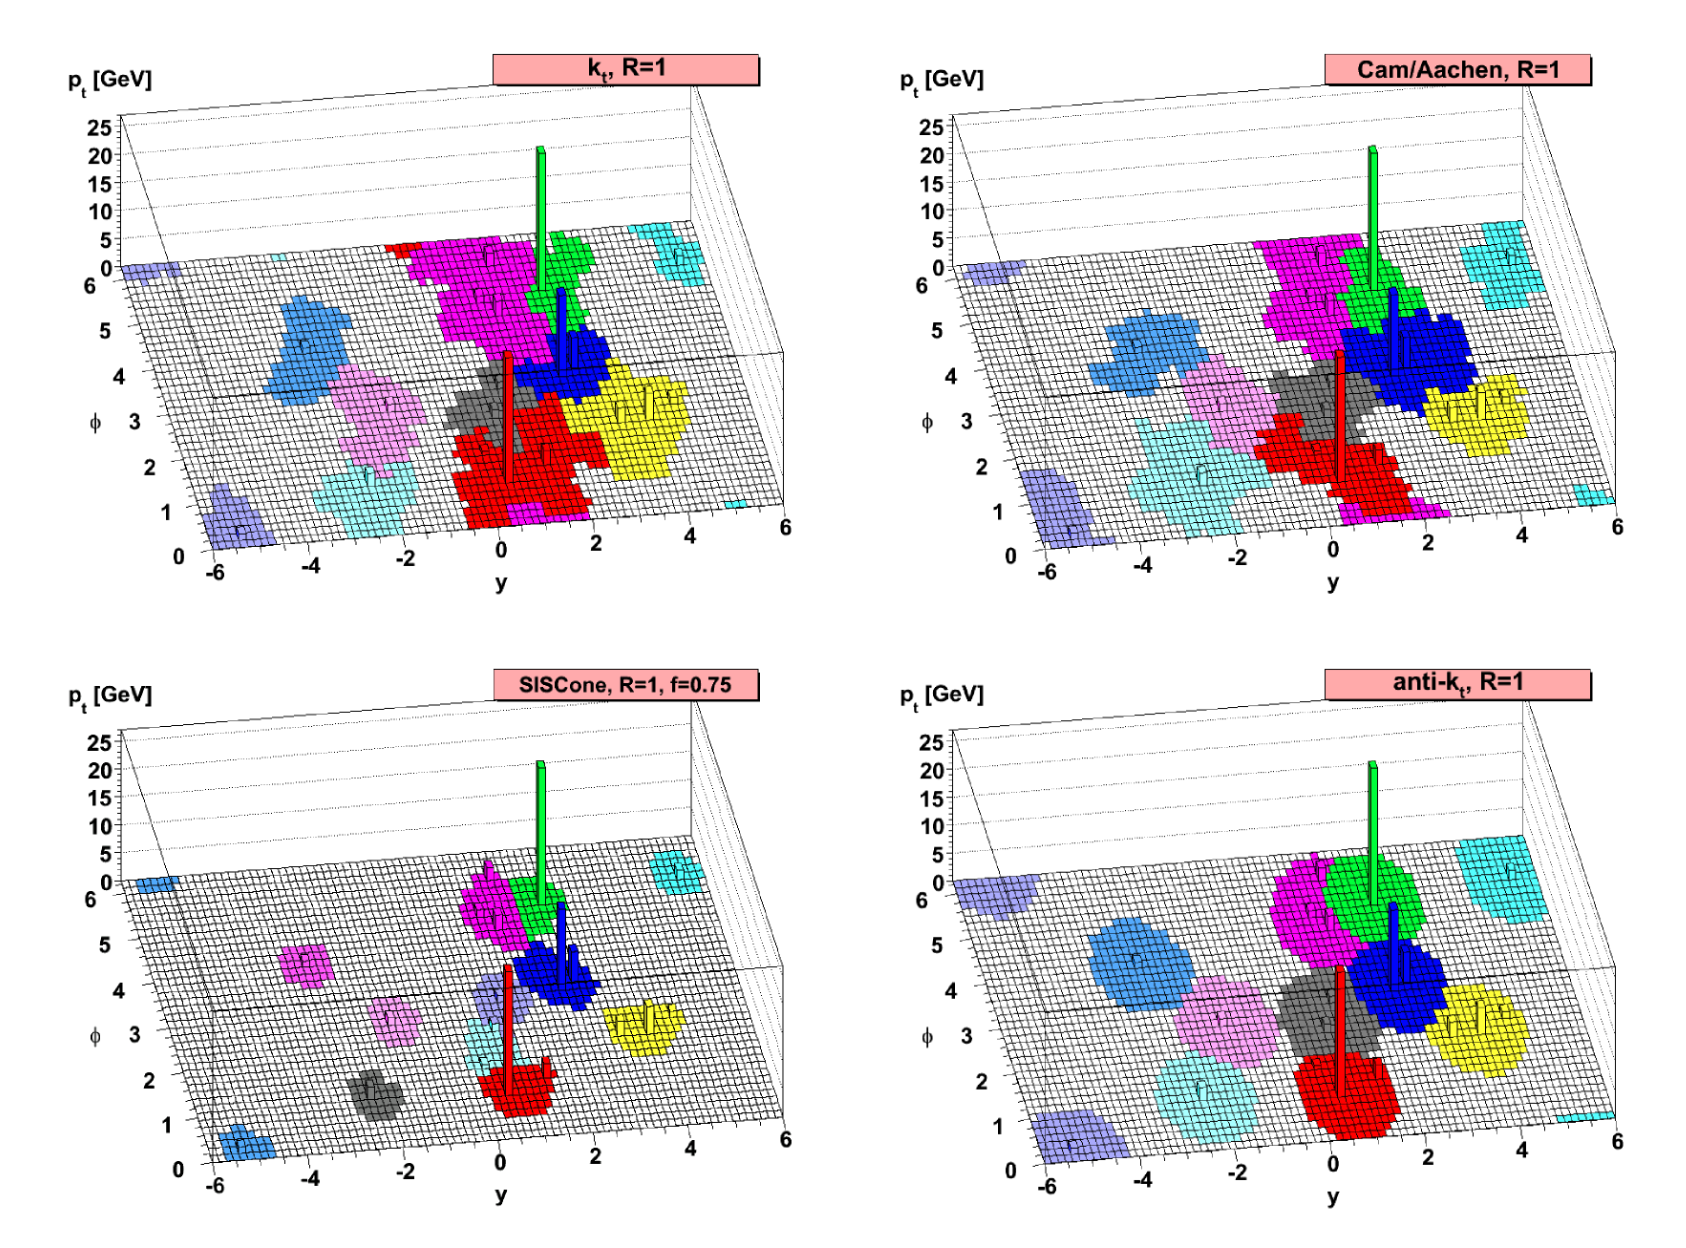
\includegraphics[height=10cm, width=13cm]{pictures/anti-kt-3D.png}
 \caption{用anti-$k_t$算法和$k_T$,Cambridge/Aachen,SISCone算法比较得到的逆反应分布。这是用Pythia6.4模拟的双喷注事件计算的,其中最硬的两个喷注满足$p_T>200[GeV]$并且都位于$\abs{y}<2$区域。逆反应对应于两个最硬喷流中每一个的净横向动量变化,这是由于当高亮度LHC堆积粒子被加入事例时非堆积粒子的重新加权(每束交叉时约有25个pp相互作用)。\cite{The_anti-kt_jet_clustering_algorithm}}
 \label{fig:3.5}
\end{figure}

对于方程\eqref{eq:dij}和方程\eqref{eq:diB}中的幂指数2p,如果我们取p=1,这就是常规的$k_T$算法,并且对于任意p>0的取值都有类似的表现,只有p=0的时候才会变成对应的“Cambridge/Aachen”算法。但是p还有一种取值,就是取p<0,这里对于所有p<0的取值,软辐射的行为都是类似的,我们专门取p=-1,并且称之为anti-$k_t$算法,也叫AK算法。R通常会取0.4、0.8、1.5三个值,分别对应的重建出的喷注名称是AK4喷注、AK8喷注、AK15喷注。

我们关心的Anti-$k_T$聚类重建算法是这么执行的:
\begin{enumerate}
    \item 在所有的距离中找到最小的距离,如果:
    \begin{enumerate}[(1)]
        \item 最小距离是来自两个物理对象i,j的距离$d_{ij}$,那我们就把这两个物理对象(i,j)从待处理列表中取出,合并定义为新喷注,再放回待处理列表;
        \item 最小距离是来自物理对象i和入射束流B之间的距离$d_{iB}$,那我们就把物理对象i定义为一个喷注,同时把它从待处理列表中移去(表示已处理完)
    \end{enumerate}
    \item 重新计算待处理列表中的所有距离(包含$d_{ij}$和$d_{iB}$两类)并重复1.步骤,直到待处理列表中没有任何物理对象存在。
\end{enumerate}
通过以上流程,我们就重建了粒子流中的所有AK喷注。



Anti-$k_T$算法与其他算法重建喷注效果比较如下\textbf{图\ref{fig:2.6}}所示
\begin{figure}[H]
 \centering
 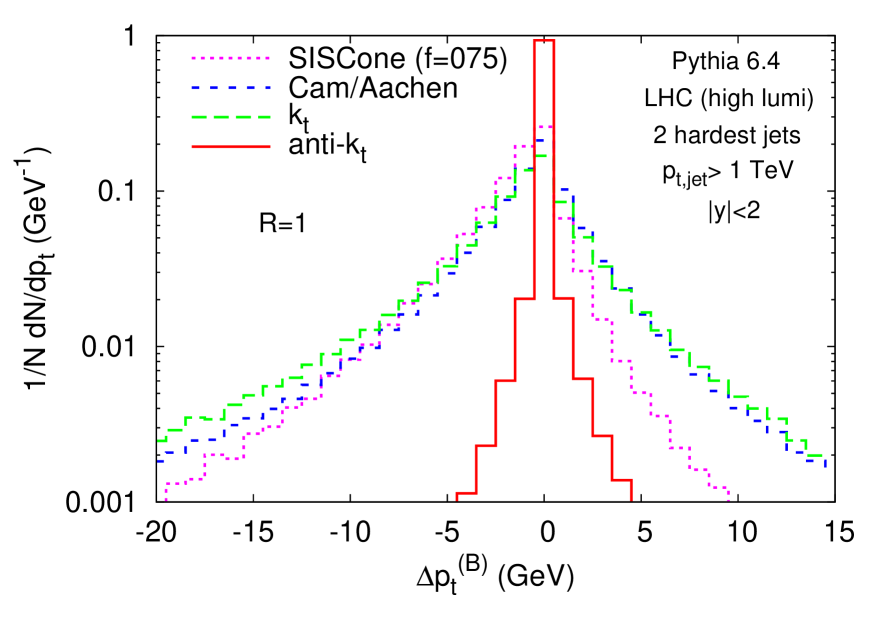
\includegraphics[height=8cm, width=10.5cm]{pictures/anti-kt.png}
 \caption{用anti-$k_t$算法和$k_t$,Cambridge/Aachen,SISCone算法比较得到的逆反应分布。这是用 Pythia 6.4 模拟的双喷注 事件计算的,其中最硬的两个喷注满足$p_T>$并且都位于$\abs{y}<2$。逆反应
对应于两个最硬喷流中每一个的净横向动量变化,这是由于当高亮度LHC堆积被加入事例时非堆积粒子的重新分配(每束交叉时约有25个pp相互作用)。\cite{The_anti-kt_jet_clustering_algorithm}}
 \label{fig:3.6}
\end{figure}
可以看到用AK算法重建出来的喷注具有更好的分辨率。

\section{喷注标记算法历史发展}
按照历史发展,对于喷注标记技术,先后出现了基于理论的高级变量算法,基于机器学习的高级变量算法和基于深度学习的初级变量算法\cite{jet-tagging-algorithms}。下面我们将分别介绍其中的代表性算法。
\subsection{基于理论的高级变量算法}
基于筛选条件的标记算法从理论灵感提供的变量出发,在实验和理论两方面都经受了广泛的研究,具有鲁棒性和易于理解和实现的特点,同时也是与新算法比较的基准线。
\subsubsection{soft-drop mass算法}
我们知道一个喷注由许多的子喷注构成,怎么取舍目标喷注中的子喷注便成了算法的核心问题。

soft-drop算法,就是丢弃掉喷注当中较软且偏离喷注中心较远的子喷注,然后计算剩余较硬且集中在喷注内部的部分的不变质量,其中,剩余的部分子喷注要满足如下的软滴条件:
\begin{itemize}
    \item soft-drop条件:
    \begin{equation}\label{eq:3.1}
        \frac{min(p_{T1}, p_{T2})}{p_{T1}+p_{T2}}>z_{cut} \left(\frac{\Delta R_{12}}{R_0}\right)^\beta
    \end{equation}
\end{itemize}
这里
\begin{equation}\label{eq:3.2}
    R_{12}=\sqrt{(\eta_1-\eta_2)^2+(\phi_1-\phi_2)^2}
\end{equation}
是子喷注1和子喷注2之间的角距离,$R_0$是要求的某个阈值。对于CMS实验,通常我们取$\beta=0$,$z_{cut}=0.1$,soft-drop条件\eqref{eq:3.1}简化为
\begin{equation}
    \frac{min(p_{T1}, p_{T2})}{p_{T1}+p_{T2}}>0.01
\end{equation}
通过soft-drop mass算法,我们可以得到我们想要的子喷注构成的喷注,从而计算出喷注对应的软滴质量(soft drop mass),软滴算法可以大大减少喷注质量分布中的“Sudakov”峰结构,使信号分辨率更明显。
\subsubsection{N-subjettiness算法}
高级变量N-subjettiness定义为
\begin{equation}
    \tau_N=\frac{1}{d_0}\sum_i p_{T,i}min\left[\Delta R_{1,i},\Delta R_{2,i},\cdots,\Delta R_{N,i}\right]
\end{equation}
这里$\Delta R_{j,i}$是指第j的子喷注到第i个子喷注的角距离。通过$\tau_N$这个变量,我们可以量化一个喷注拥有N个子喷注的兼容性。

进一步地,我们可以通过不同$\tau_N$之间的比值获得更有鉴别效果的变量,例如
\begin{enumerate}[(1)]
    \item 定义
    \begin{equation}
        \tau_{21}=\frac{\tau_2}{\tau_1}
    \end{equation}
    可以针对鉴别二分叉喷注(如W,Z,H)。
    \item 定义
    \begin{equation}
        \tau_{32}=\frac{\tau_3}{\tau_2}
    \end{equation}
    可以针对鉴别三分叉喷注(如top),同时对top喷注的b夸克子喷注还可以运用$\tau_{21}$来进一步改善效果。
\end{enumerate}
在重建中,我们一般在应用soft-drop mass算法后计算喷注的ECF比率,这提高了 ECF 作为喷注质量和$p_T$函数的稳定性。

\subsubsection{ECF:$N_2$算法}
这里我们要用到泛化能量关联函数(ECF),对于一个包含$N_c$个子喷注的喷注,它的ECF如下定义
\begin{equation}
    {}_{q}e_{N}^{\beta}=\sum_{1\leq i_{1}<i_{2}<\cdots<i_{N}\leq N_{\text{C}}}%
\left[\prod_{1\leq k\leq N}\frac{\pt^{i_{k}}}{\pt^{J}}\right]\prod_{m=1}^{q}%
\min_{i_{j}<i_{k}\in\{i_{1},i_{2},\cdots,i_{N}\}}^{(m)}\left\{\Delta R_{i_{j},%
i_{k}}^{\beta}\right\}
\end{equation}
这个变量可以用来测试喷注有N个辐射中心的兼容性,与N-subjettiness变量有点相似,但是ECF是无轴方法,并且对于N分叉喷注,如果$N>M$,我们会有$e_N\gg e_M$。

对于二分叉标记喷注(W/Z/H),可以定义ECF比值为
\begin{equation}
    N_{2}^{1}=\frac{{}_{2}e_{3}^{1}}{(_{1}e_{2}^{1})^{2}}
\end{equation}
与N-subjettiness比值$\tau_{21}$相比, 其优点是它作为喷注质量和$p_T$的函数更稳定,这种方法也被称为“$m_{SD}+N_2$”算法。

本算法还有质量去相关的版本,便于压低峰状本底,具体做法如下,定义“设计去相关标记器”变量为
\begin{equation}
    N_2^{DDT}(\rho,p_T)=N_2(\rho, p_T)-N_2^{(X\%)}(\rho,p_T)
\end{equation}
此处$\rho=\ln{(m_{SD}^2/p_T^2)}$是一个无量纲变量,$N_2^{(X\%)}$是
模拟QCD样本中$N_2$分布的X百分位的取值。这确保了筛选条件$N^{DDT}_2<0$会导致在考虑的质量与横向动量范围内QCD的标记效率为恒定X\%,并且没有标记性能上的损失。

\subsection{基于机器学习的高级变量算法}
\subsubsection{$N_3$-BDT算法}
我们想考虑具有尺度不变性的ECF比率,可以通过以下式子定义的变量来构造:
\begin{equation}
    \frac{{}_{a}e_{N}^{\alpha}}{(_{b}e_{M}^{\beta})^{x}}\text{, where }M\leq N%
\text{ and }x=\frac{a\alpha}{b\beta}.
\end{equation}
对于top夸克喷注标记算法,仅考虑彼此不高度相关的那些变量,并且丢弃无法很好被模拟定义的比值变量,这样我们得到如下11个比值变量
\begin{equation}
\begin{split}
\displaystyle\frac{{}_{1}e_{2}^{(2)}}{\Bigl{(}{}_{1}e_{2}^{(1)}\Bigr{)}^{2}},%
\frac{{}_{1}e_{3}^{(4)}}{{}_{2}e_{3}^{(2)}},\frac{{}_{3}e_{3}^{(1)}}{\Bigl{(}{%
}_{1}e_{3}^{(4)}\Bigr{)}^{3/4}},\displaystyle\frac{{}_{3}e_{3}^{(1)}}{\Bigl{(}{}_{2}e_{3}^{(2)}\Bigr{)}^{3/4}}%
,\frac{{}_{3}e_{3}^{(2)}}{\Bigl{(}{}_{3}e_{3}^{(4)}\Bigr{)}^{1/2}},
\displaystyle\frac{{}_{1}e_{4}^{(4)}}{\Bigl{(}{}_{1}e_{3}^{(2)}\Bigr{)}^{2}},\\
\frac{{}_{1}e_{4}^{(2)}}{\Bigl{(}{}_{1}e_{3}^{(1)}\Bigr{)}^{2}},\frac{{}_{2}e_%
{4}^{(1/2)}}{\Bigl{(}{}_{1}e_{3}^{(1/2)}\Bigr{)}^{2}},\displaystyle\frac{{}_{2}e_{4}^{(1)}}{\Bigl{(}{}_{1}e_{3}^{(1)}\Bigr{)}^{2}},%
\frac{{}_{2}e_{4}^{(1)}}{\Bigl{(}{}_{2}e_{3}^{(1/2)}\Bigr{)}^{2}},\frac{{}_{2}%
e_{4}^{(2)}}{\Bigl{(}{}_{1}e_{3}^{(2)}\Bigr{)}^{2}}.
\end{split}
\end{equation}
基于ECF的top夸克标记器,称为“$N_{3}\text{-}\mathrm{BDT}\,(\mathrm{CA}15)$”,使用扩展决策树模型,以这11个ECF比值变量加上,$\tau^{SD}_{32}\text{和}f_{rec}$作为输入。

\subsubsection{HOTVR算法}
全称为“带R变量的重对象标记器”(Heavy Object Tagger with Variable R),带$p_T$无关的变量距离参数$R$的喷注簇射和经过Puppi算法修正Pile-up的ParticleFlow候选者,在这个过程中,软簇射会被丢弃掉,从而得到稳定的喷注质量分布,同时阻止额外的辐射进入喷注。

可以被用于标记不同的重共振态(t/W/Z/H)。
\subsubsection{BEST算法}
全称是“扩展事例形状标记器”(Boosted Event Shape Tagger),是针对top/W/Z/Higgs的多分类标记器,在参考坐标系中计算喷注运动学/形状的变量,,并且把参考坐标系分别按top/W/Z/Higgs喷注假设变换成四个静止坐标系,如果被变换到了正确的静止坐标系,那么喷注的子组分就应该是各向同性并且会展示出预期的N分叉结构。

我们使用神经网络训练这些运动学变量和子喷注的b标记判别式,这个神经网络由三个全连接层构成,每层带有40个节点。
\subsection{基于深度学习的初级变量算法}
这里实际上已经开始进入深度学习时代,基于深度学习的新标记算法在最近几年已经被提上预案并且受到了大量关注,基本思想就是使用初级变量加上深度神经网络,对于喷注标记,有两种深度神经网络的路径:
\begin{enumerate}
    \item \textbf{基于图像}:\label{dl:image}\\
    把喷注转化为使用量能器能量沉积得到的图像,利用计算机视觉技术——通常是二维卷积神经网络。但是由于图像的稀疏性和异构探测器,仍然挑战和困难重重。
    \item \textbf{基于粒子}:\label{dl:particle}\\
    把喷注当成它自己组分粒子的集合,这样可以利用循环神经网络,一维卷积神经网络和图神经网络等等技术。同时还可以通过CMS的Particle-Flow重建流程产生诱导出更多自然的想法,合并所有子探测器的信息并且充分利用粒度。
\end{enumerate}

现在这两条算法路径在CMS实验中都在开发,以下将通过两个例子分别介绍这两条路径的情况。
\subsubsection{IamgeTop算法}
这是基于喷注图像的top夸克标记算法,喷注图像基于喷注横向动量自适应缩放以
增加高$p_T$区域的准直。喷注图像有四个“颜色”通道:(1)中性$p_T$(2)径迹$p_T$(3)$\mu$子个数(4)径迹条数。此算法还利用了深度喷注b夸克标记的判别式。

\textbf{质量去相关的ImageTop算法}:
训练时重新加权QCD样本使得本底的质量分布与top夸克的质量分布相匹配,从而获得ImageTop-MD标记器。
\subsubsection{DeepAK8算法}
DeepAK8是基于AK8喷注针对top/W/Z/Higgs标记任务的多分类标记器,其中还会按照衰变道进行进一步的子分类(例如,$Z\to bb$,$Z\to cc$,$Z\to qq$等)。
此算法直接用喷注组分(如ParticleFlow候选者,二级顶点等)作为输入,采用一维卷积神经网络作为架构

\textbf{质量去相关的DeepAK8算法}:
使用对抗训练技术,训练时重新加权本底样本和信号样本获得$m_{SD}$和$p_T$的二维平分布以辅助训练。
	\chapter{用于喷注标记的ParticleNet深度神经网络}
\label{chap4}
\fontsize{12bp}{14.4pt}

喷注是是LHC(大型强子对撞机)上无处不在且蕴含大量粒子信息的物理对象,因此,关于喷注的标记就是许多潜在新物理的探寻与标准模型测量检验的关键,而喷注标记任务主要分为以下三类:
\begin{enumerate}
    \item 重夸克喷注标记
    \item 重共振态标记
    \item 夸克/胶子的区分鉴别
\end{enumerate}

而分类标记任务,也是机器学习领域最活跃的方向之一。因此,要结合以上两个领域,关键性的问题就是:\textbf{怎样尽可能物理地把喷注表示成机器学习中的对象?}
\section{喷注表示方式}
从深度学习的计算机视觉领域出发,最经典的方式是表示成图像,如\ref{dl:image}所介绍。还有一种路径是把喷注表示成粒子的集合,如\ref{dl:particle}所介绍。这两种路径的表示方法在CMS实验分析中已经有了相关的探索和标记器的开发。但我们还应该保持好奇:是否还有更好的表示方法和与之对应更好的网络架构呢?

这就是我们开发的标记器所采用的喷注表示方法的基础:点云(Paticle Clouds)。点云,就是空间中数据点的集合,这类数据结构的收集方式是通过三维扫描测量物体表面周围的大量点而得到。但对于我们关心的物理喷注,应当不仅仅用点云,或者说,应该用点云的一个喷注适应版:粒子云\cite{PaticleNet}(Particle Cloud)。

喷注(或者说,粒子云)就是空间中粒子的集合。粒子云的收集方式是用粒子探测器测量到的大量粒子的聚类。

经过喷注适应后的粒子云表示方式和点云表示方式有如下的关联:
\begin{itemize}
    \item 共同点:点云中的点和粒子云中的粒子都是内禀无序的。
    \item 不同点:点云中的基本信息是xyz空间的3维坐标;粒子云中的基本信息是$\eta-\phi$空间的二维坐标,但同时还具有许多其他特征,如:能动量,电荷,粒子鉴别(Particle ID),径迹质量,探测器受击参数等。
\end{itemize}
粒子云的置换对称性使其成为喷注最自然和有希望的表示。为了实现粒子云表示的最佳性能,必须仔细设计神经网络的架构以充分利用这种表示的潜力。在本节中,我们将介绍ParticleNet,这是一种类似于CNN的深度神经网络,使用粒子云数据进行喷注标记。
\section{边卷积(EdgeConv)}
CNN在计算机视觉的各种机器学习任务中取得了压倒性的成功。CNN的两个关键特征对其成功做出了重大贡献。首先,卷积操作通过在整个图像中使用共同核函数来利用图像的平移对称性。这不仅大大减少了网络中的参数数量,而且可以更有效地学习参数,因为每个卷积矩阵都会使用图像的所有位置进行学习。其次,CNN利用分层方法学习图像特征。卷积操作可以有效堆叠形成深度网络。CNN中的不同层具有不同的感知范围,因此可以学习不同尺度的特征,浅层利用局部定域信息,深层学习更多全局结构。这种分层方法被证明是了一种学习图像的有效方法。

受到CNN的启发,ParicleNet中采用了类似的方法来学习粒子云数据。然而,常规的卷积运算不能应用于粒子云,因为粒子云中的点可以不规则不均匀地分布,而不是像图像中的像素一样被划分为均匀的网格。因此对于粒子云结构,其卷积操作的基础,即卷积核函数如何作用于不均匀不规整的局域数据点,仍然有待定义。此外,一个通常的卷积操作,是这样的形式$\sum_{i}K_{i}x_{i}$,这里$x_i$
表示局域某个点的特征,$K_i$是核函数对应该点的矩阵元。我们可以看到,这个形式在点的置换操作下是会变的(交换$x_i$,$x_j$而不交换$K_i$,$k_j$)。因此,适应于粒子云的“卷积”操作也需要修改以考虑到粒子云内的交换对称性。

边卷积(EdgeConv)操作\cite{edgeconv}被提出作为点云结构的类卷积操作。EdgeConv 首先将点云表示为图结构,其顶点(Vertex)是点本身,为每个点与其k个最近的相邻点的连线被构造为图的边(Edge)。这样,为每个点定义了点云卷积所需的局部补丁作为与之相连的最近邻点。每个点的EdgeConv操作有形式
\begin{equation}\label{eq:4.1}
    \bm{x}_{i}^{\prime}=\mathop{\square}\limits_{j=1}^{k}\bm{h}_{\bm{\Theta}}(\bm{x}_{i},\bm{x}_{i_{j}}),
\end{equation}
这里$\bm{x}_{i}\in\mathbb{R}^{F}$表示点$x_i$的特征向量,$\{i_{1},...,i_{k}\}$是点$x_i$的k最近邻点的索引,边函数$\bm{h}_{\bm{\Theta}}:\mathbb{R}^{F}\times\mathbb{R}^{F}\rightarrow\mathbb{R}^{F^{\prime}}$代表着一系列可被$\bm{\Theta}$参数化的函数,且$\bm{\Theta}$本身属于可学习参数。$\square$是逐通道的对称聚合操作(例如max,mean,sum等)。并且边函数$\bm{h_\Theta}$对于点云中的所有点都是相同的,这样和对称聚合操作$\square$一起使边卷积(EdgeConv)成为了点云上的置换对称操作。

在ParticleNet模型中,遵循了以上原则,并且使用了特殊化的边函数
\begin{equation}
    \displaystyle\bm{h}_{\bm{\Theta}}(\bm{x}_{i},\bm{x}_{i_{j}})=\displaystyle{Conv}_{\bm{\Theta}}(\bm{x}_{i},\bm{x}_{i_{j}}-\bm{x}_{i})=\displaystyle\sum_{c}\theta_{c}^{~{}a}x_{i,c}+\sum_{c}{\theta^{\prime}}_{c}^{~{}a}(x_{i_{j},c}-x_{i,c})
\end{equation}
在这里,方程\eqref{eq:4.1}中的邻点的特征向量$\bm{x}_{i_{j}}$被$\bm{x}_{i_{j}}$与中心点的特征向量$\bm{x}_{i}$的差值所取代,并且$Conv_{\bm{\Theta}}$仅是常规形式下特征向量的加权和。c是输入特征向量序列的索引,a是核函数序列的索引。对于方程\eqref{eq:4.1}中的对称聚合操作$\square$,ParticleNet采取的是平均值$\frac{1}{k}\sum$。

\begin{figure}[H]
 \centering
 \caption{边卷积(EdgeConv)操作的结构\cite{PaticleNet}}
 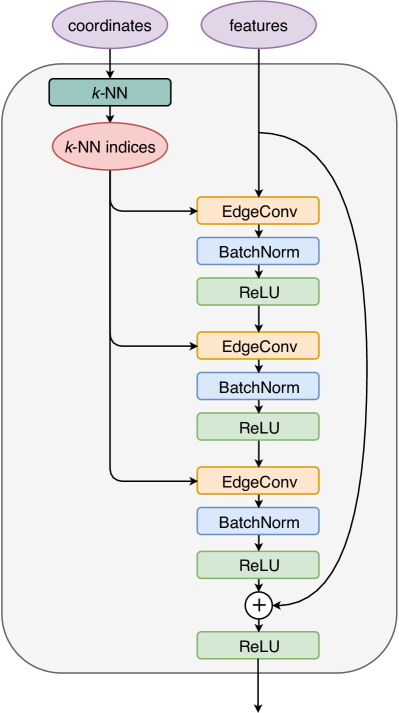
\includegraphics[height=14cm, width=8cm]{pictures/edgeconv.png}
 \label{fig:4.1}
\end{figure}

EdgeConv 操作的一个重要特点是它可以很容易地堆叠,就像常规卷积一样。这是因为 EdgeConv可以看作是从一个点云到另一个具有相同数目点的点云的映射,只是可能会改变每个点的特征向量的维度。因此,随后可以应用另一个 EdgeConv 操作。这使我们能够使用EdgeConv操作构建一个深度网络,该操作可以分层学习点云的特征。

EdgeConv 操作的可堆叠性也带来了另一个有趣的可能性。基本上,EdgeConv 学习到的特征向量可以看作是潜在空间中原始点的新坐标,然后是点之间的距离(用于判断最近的邻居)可以在这个潜在空间中重新定义。换句话说,点的接近程度可以动态地通过EdgeConv操作学习到。这也是了动态图卷积神经网络的结果Wang(2018)。其中描述点云的图被动态更新以反映边的变化,即每个点的邻居,这也得到证明比保持静态图 的性能更好。Wang等人(2018) .

\section{ParticleNet网络架构}
ParticleNet架构大量使用了EdgeConv操作,也采用了动态图更新方法。然而,与原始的Dynamic Graph CNN相比,ParticleNet中做出了许多不同的设计选择,以更好地适应喷注标记任务。

\begin{figure}[H]
 \centering
 \caption{ParticleNet深度网络架构\cite{PaticleNet}}
 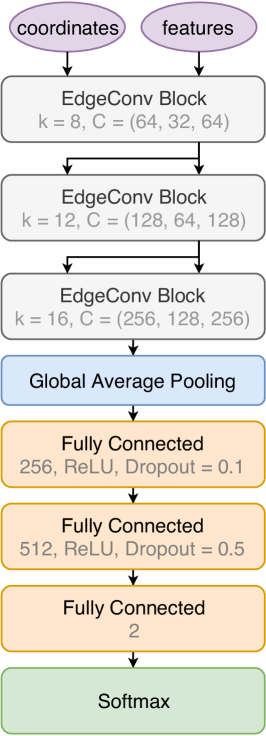
\includegraphics[height=14cm, width=5cm]{pictures/ParticleNet_Architecture.png}
 \label{fig:4.2}
\end{figure}

我们在 EdgeConv 操作块中构建 ParticleNet 架构。图1说明了 EdgeConv 块的结构。EdgeConv 块从找到每个粒子的最近相邻粒子。使用 EdgeConv 块的坐标输入计算粒子之间的距离。然后,对粒子的输入特征向量应用 EdgeConv 操作。每个块由多个 EdgeConv 操作组成,可能具有不同数量的卷积核。在每个块内,描述粒子云的图是固定的,即一个粒子总是有相同的最近的邻居。每个 EdgeConv 操作后面都有一个批量归一化层BatchNorm【Ioffe 和 Szegedy (2015)】然后是 ReLU 非线性Glorot 等人。(2011) . 与 ResNet 类似,与 EdgeConv 操作并行运行的快捷连接也包含在每个块中。


本文使用的 ParticleNet 架构如\textbf{图\ref{fig:4.2}}所示。它由三个 EdgeConv 块组成。第一个EdgeConv块使用伪快速度-方位角空间中粒子的空间坐标来计算距离,而随后的块使用学习的特征向量作为坐标。最近邻居的数量对于三个块,分别为 8、12 和 16。每个块由三个 EdgeConv 层组成。三个块的 EdgeConv 层的输出通道数为 (64, 32, 64), (128, 64, 128) 和 (256, 128, 256)。在 EdgeConv 块之后,应用全局平均池化操作来聚合云中所有粒子的学习特征。接下来是两个全连接层,分别有 256 和 512 个单元。两者都使用 ReLU 激活函数。两个带有dropout概率分别为0.1和0.5的dropout层用来以防止过度拟合。然后是具有2个单元的全连接层,后跟一个softmax函数,用于生成二分类任务的输出。


	\chapter{开发首个$H\to WW$质量去相关的多分类标记器(基于ParticleNet)}
\label{chap5}
\fontsize{12bp}{14.4pt}

\section{质量去相关技术}
对于质量相关版本的标记器,神经网络会学习到信号样本与本底样本质量分布的差异,并且把它作为区分信号与本底的潜在判别条件,对于这样训练出来的标记器,在把本底事件误鉴别为信号事件时,会更倾向于挑选出质量分布接近信号样本的本底事件,从而对于数据中通过标记器的本底事件,在质量谱上会形成信号峰下的峰状本底,这种情况也叫做质量雕刻(mass-sculpting)。这显然对于我们从质量谱中提取信号造成了不小的困难,因此质量去相关的标记器就显得尤为重要。

从以上信息我们知道,当训练中的信号和本底样本有明显不同的质量分布时,训练出来的标记器在推理筛选本底样本时就会出现质量雕刻的现象。所以,如果训练样本的信号和本底的质量分布一致,标记器则不会学习到二者的质量信息作为区分条件,从而不会在推理筛选本底样本时出现质量雕刻现象。

要实现这点,最简单直接的办法就是在训练时对信号和本底的分布进行重新加权,但是这往往还有其他隐患,例如:
\begin{enumerate}[(1)]
    \item 如果信号样本的质量分布峰过于集中,也就是说,在信号质量窗外的事例统计量过低,这样对信号重加权时,会导致信号窗内的高峰被极大压低到和信号窗外事件相同的高度,从而造成大量真实信号没有被选中参与训练,是一种极大的浪费和欠拟合的隐患。
    \item 同时,对于远离信号窗的事例,也很难被重建出来,进一步加大了训练和推理的难度。
\end{enumerate}
综合以上两点原因,最好的做法就是尽可能使用于训练的信号样本的质量分布尽可能平滑(避免极端事例的低统计量过度压低加权),信号窗尽可能大(避免远离信号窗事例难以重建)。所以我们的做法是:设计带有一维$ m_{SD}$平分布的专用MC样本以供训练,可以通过产生并合并不同共振态质量的样本实现。(例如,产生变质量$m_X$的$X\to bb$,$X\to cc$,$X\to qq$样本以训练通用二分叉喷注标记)

\section{分类标签}
\subsection{信号分类标签}
对于我们关心的$H\to WW\to anything$的信号,我们主要关心两种衰变场景:一种是两个W都进行强子化衰变,也称作全强子衰变;另一种是一个W进行强子化衰变一个W进行轻子化衰变,也被称作半轻衰变)。所以,我们采用了以下的末态分类标签:
\begin{itemize}
    \item $\mathbf{4q}$:$H\to W(2q)W(2q)$,并且重建出4分叉的AK8喷注
    \item $\mathbf{3q}$:$H\to W(2q)W(2q)$,但仅重建出3分叉的AK8喷注
    \item $\mathbf{e\nu_e qq}$:$H\to W(e\nu_e)W(2q)$喷注
    \item $\mathbf{\mu\nu_\mu qq}$:$H\to W(\mu\nu_\mu)W(2q)$喷注
    \item $\mathbf{\tau_e\nu_eqq}$:$H\to W(\tau\nu)W(2q)$,$\tau$接着衰变为电子等产物
    \item $\mathbf{\tau_\mu\nu qq}$:$H\to W(\tau\nu)W(2q)$,$\tau$接着衰变为$\mu$子等产物
    \item $\mathbf{\tau_h\nu qq}$:$H\to W(\tau\nu)W(2q)$,$\tau$接着进行强子化衰变
\end{itemize}
\subsection{本底分类标签}
对于我们关注的QCD本底喷注,我们可以按喷注中的子喷注结构对其进行分类如下:
\begin{itemize}\label{eq:5.2}
    \item \textbf{QCD(bb)}:QCD喷注中有两个b夸克子喷注
    \item \textbf{QCD(cc)}:QCD喷注中有两个c夸克子喷注
    \item \textbf{QCD(b)}:QCD喷注中有一个b夸克子喷注
    \item \textbf{QCD(c)}:QCD喷注中有一个c夸克子喷注
    \item \textbf{QCD(others)}:具有其他子结构的QCD喷注
\end{itemize}
\section{数据集}
\subsection{训练集和验证集}
我们产生了专门设计的私人HWW信号样本和基于官方设置产生的QCD本底样本,同时按照15:1的比例把它们分成训练集和验证集供训练使用。
\subsubsection{信号样本}
因为我们的目标是开发一个质量去相关的标记器,所以我们的信号MC样本有以下特点:
\begin{enumerate}
    \item 样本基于2017 ultra-legacy,总共有两千五百多万事例。
    \item 使用变质量X的$X\to WW$衰变样本,设置的产生级别质量分布区间为$15 [\si{GeV}]\leq m_X\leq 250[\si{GeV}]$,并保证合并起来的总信号样本具有平坦的产生级别质量分布,同时设置W质量为$m_W=80[\si{GeV}]$。
    \item 使用JHUGen产生子实现$X\to WW\to4q/\ell \nu qq$衰变以更好模拟衰变产物的自旋关联。
    \item 喷注经过AK8算重建法并且通过MC事实匹配打上标签。
\end{enumerate}

\subsubsection{本底样本}
QCD本底样本有以下几个特点:
\begin{enumerate}
    \item 样本基于2017 ultra-legacy,总共有两千八百多万事例。
    \item 喷注经过AK8算重建法并且通过MC事实匹配打上标签。
\end{enumerate}
\subsection{测试集}
测试集以训练集和验证集相同的方式产生。

对于测试集中的信号样本,Higgs的产生级别质量固定在标准模型125[GeV]处(训练集中不包含这个质量点产生的样本),包含约四十万个事例。

对于测试集中的QCD本底样本,以和训练集相同的方式产生,共有约五百万左右事例。


\section{标注器设置}
\subsection{预挑选条件}
我们要求进入标注器的事例满足以下条件:
\begin{enumerate}
    \item 每个事例仅由一个喷注构成,并且这个喷注通过了Pile-up的紧挑选条件
    \item 喷注的横向动量满足$200[\si{GeV}]<p_T<2500[\si{GeV}]$
    \item 喷注的soft-drop质量满足$20[\si{GeV}]\leq m_{SD}<260[\si{GeV}]$
    \item 对于训练样本,喷注要通过事实匹配满足12个标签分类之一
\end{enumerate}
\subsection{重加权设置}
训练用的信号样本和本底样本合起来共有12个分类标签,我们要产生质量去相关的标记器,就得对用于训练的信号和本底进行质量和横向动量的二维分区间重加权。

\textbf{重加权的定义}是:对于某个被重加权的标签分类,指定分布上的每个区间都要持有相同数量的事例数,并且来自每个分类的事例数占比要符合我们预定义的分类权重

现在我们要对信号和QCD本底样本同时在$[p_T,m_{SD}]$二维分布上做重加权操作,对soft-drop质量$m_{SD}$的分bin区间为从20[GeV]到260[GeV]每隔10[GeV]分一个bin,对横向动量$p_T$的分bin区间为[200, 251, 316, 398, 501, 630, 793, 997, 1255, 1579, 1987, 2500],单位为[GeV]。(值得注意的是,对$p_T$分bin按照对数等bin宽的选择,这是因为有对QCD的$p_T$分布呈指数衰减的经验分布,所以采用对数等bin宽可以尽可能使得分bin后直方图高度均匀)

定义各个分类标签定义的重加权权重时,我们把\eqref{eq:5.2}中的五个QCD子分类都合并成$QCD$标签分类参与加权。最后得到分类权重的如下:
\begin{equation}
\begin{split}
    4q:3q:e\nu qq:\mu\nu qq:\tau_e\nu qq:\tau_\mu\nu qq:\tau_h\nu qq:QCD \\
    =0.34:0.08:0.2:0.2:0.03:0.03:0.12:1 &
\end{split}
\end{equation}
这里各个信号子分类的权重经过我们精心挑选,使得每个权重与该分类在信号中的占比接近,从而提高训练速度。

\subsection{神经网络输入}
\begin{table}[htbp]
    \caption{神经网络输入}
    \centering
    \begin{tabular}{>{\centering\arraybackslash}p{2.5cm}%
    >{\centering\arraybackslash}p{3cm}%
    >{\centering\arraybackslash}p{9cm}}
    \toprule\toprule
    \textbf{对象} & \textbf{变量} & \textbf{描述}\\
    \midrule
    \multirow{25}{*}{粒子候选者} & $\eta_{rel}$ & 相对于AK8喷注主轴的赝快度$\Delta \eta$\\
    & $\phi_{rel}$ & 相对于AK8喷注主轴的方位角$\Delta \phi$\\
    & $\log{p_T}$ & $p_T$的对数\\
    & $\log{E}$ & 能量的对数\\
    & $|\eta|$ & 赝快度的绝对值\\
    & charge & 电荷\\
    & isEl & 是否被鉴别为电子\\
    & isMu & 是否被鉴别为$\mu$子\\
    & isGamma & 是否被鉴别为光子\\
    & icChargedHad & 是否被鉴别为带电强子\\
    & isNeutralHad & 是否被鉴别为中性强子\\
    & VTX\_ass & 初级顶点的关联品质\\
    & lostInnerHits & 内部硅径迹器的击中数信息\\
    & normchi2 & 径迹拟合的归一化$\chi^2$\\
    & quality & 径迹品质\\
    & dz & 纵向冲击参数:在z方向到初级顶点的最近距离\\
    & dzsig & 纵向冲击参数显著度\\
    & dxy & 横向冲击参数:在横切面到束流的最近距离\\
    & dxysig & 横向冲击参数显著度\\
    & BTag\ $\eta_{rel}$ & 径迹相对AK8喷注主轴的赝快度$\Delta \eta$\\
    & BTag\ $p_T$ ratio & 径迹垂直AK8喷注主轴的分动量与合动量之比\\
    & BTag $p_{\parallel}$ Ratio & 径迹平行AK8喷注主轴的分动量与合动量之比\\
    & BTag Sip3dVal & 径迹的三维正负冲击参数\\
    & BTag Sip3dSig & 径迹的三维正负冲击参数显著度\\
    & BTag JetDistVal & 径迹到AK8喷注主轴的最小接近距离\\
    \midrule
    \multirow{11}{*}{次级顶点} & $\eta_{rel}$ & 相对于AK8喷注主轴的赝快度$\Delta \eta$\\
    & $\phi_{rel}$ & 相对于AK8喷注主轴的方位角$\Delta \phi$\\
    & $m_{SV}$ & 次级顶点不变质量\\
    & $\log{p_T}$ & $p_T$的对数\\
    & $|\eta|$ & 赝快度的绝对值\\
    & $N_{track}$ & 径迹条数\\
    & normchi2 & 顶点拟合的$\chi^2$除以自由度\\
    & dxy & 横向飞行距离\\
    & dxysig & 横向飞行距离显著度\\
    & d3d & 三维飞行距离\\
    & d3dsig & 三维飞行距离显著度\\
    \bottomrule\bottomrule
\end{tabular}
\end{table}

\section{标记器在测试集上效果}
ROC图如下
\begin{figure}[H]\label{fig:5.2}
 \centering
 \caption{标记器的$H\to WW\to 4q$标记效果}
 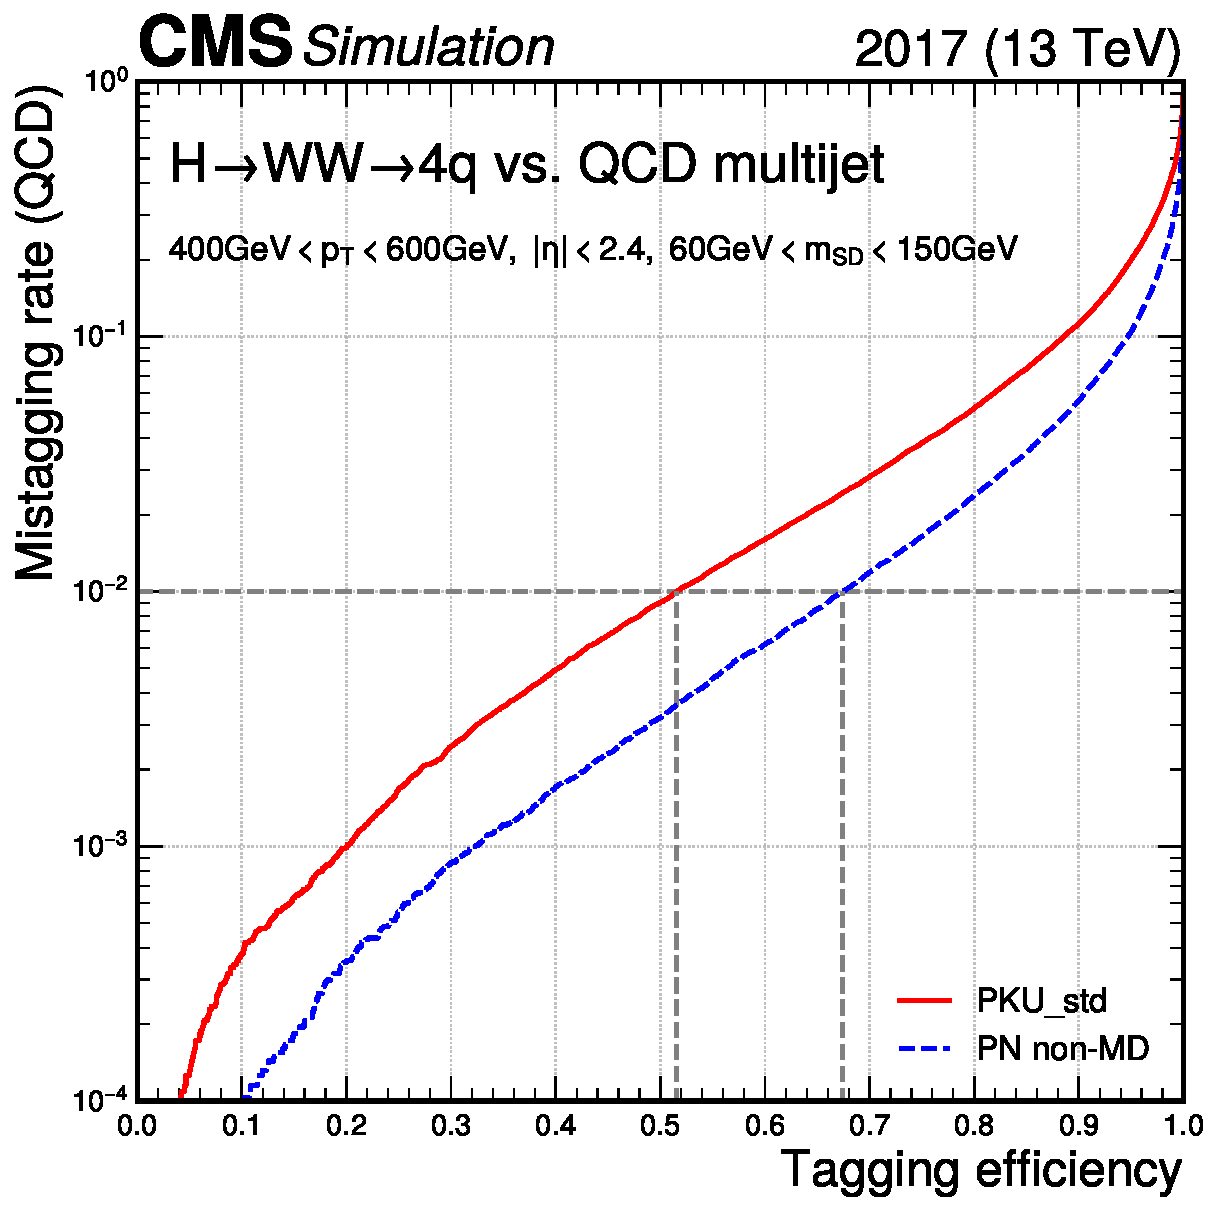
\includegraphics[height=12cm, width=12cm]{pictures/ROC_HWW_4q.pdf}
\end{figure}
这里PKU\_std是我们开发的质量去相关版本HWW多分类标记器,PN non-MD是原生ParticleNet的质量相关版本HWW4q单道标记器。在$Mistag\ rate=1\%$时,PKU\_std的Tagging efficiency$\approx52\%$,PN non-MD的Tagging efficiency$\approx68\%$。虽然PKU\_std比PN non-MD的效果要稍微差一些,但这正是质量去相关标记器的代价,换来的是被误鉴别的QCD本底没有接近信号峰的质量雕刻。如\textbf{图\ref{fig:5.3}}所示。

从\textbf{图\ref{fig:5.3}}可以看到,我们开发的质量去相关标记器的质量去相关效果非常好,在4q喷注的信号峰附近,QCD本底仍然保持了它原本的分布,没有形成类似4q喷注的质量峰分布,从而有利于我们在实验数据中提取4q信号。
而被PN non-MD误标记的QCD本底就有非常明显的质量雕刻现象,如\textbf{图\ref{fig:5.4}}所示。

比较以上两图我们可以看到,虽然PKU\_std比PN non-MD的效果要稍微差一些,但这正是质量去相关标记器的代价,以效率上20\%的损失换来了从无到有的质量去相关效果,极大地降低了分析难度。
\begin{figure}[H]
 \centering
 \caption{被PKU\_std误标记的QCD本底的$m_{SD}$分布}
 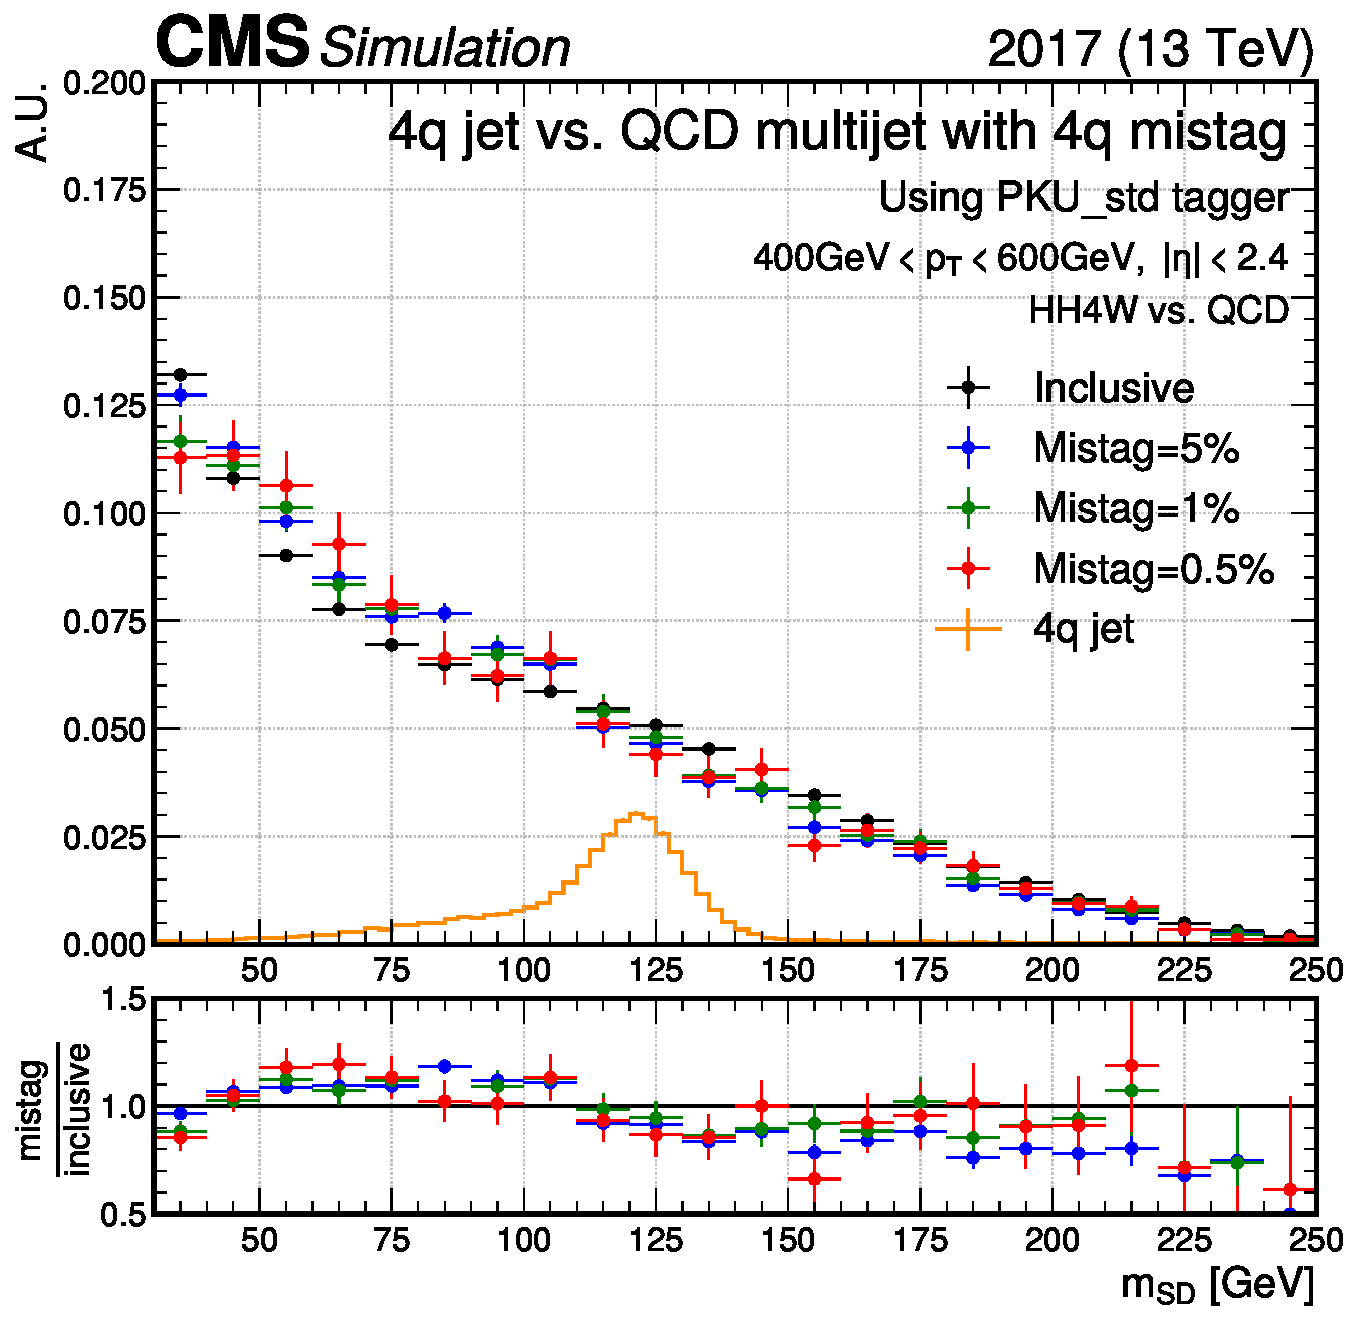
\includegraphics[height=10.5cm, width=10.5cm]{pictures/MD_PKU_std_4q.pdf}
 \label{fig:5.3}
\end{figure}

\begin{figure}[H]
 \centering
 \caption{被PN nonMD误标记的QCD本底的$m_{SD}$分布}
 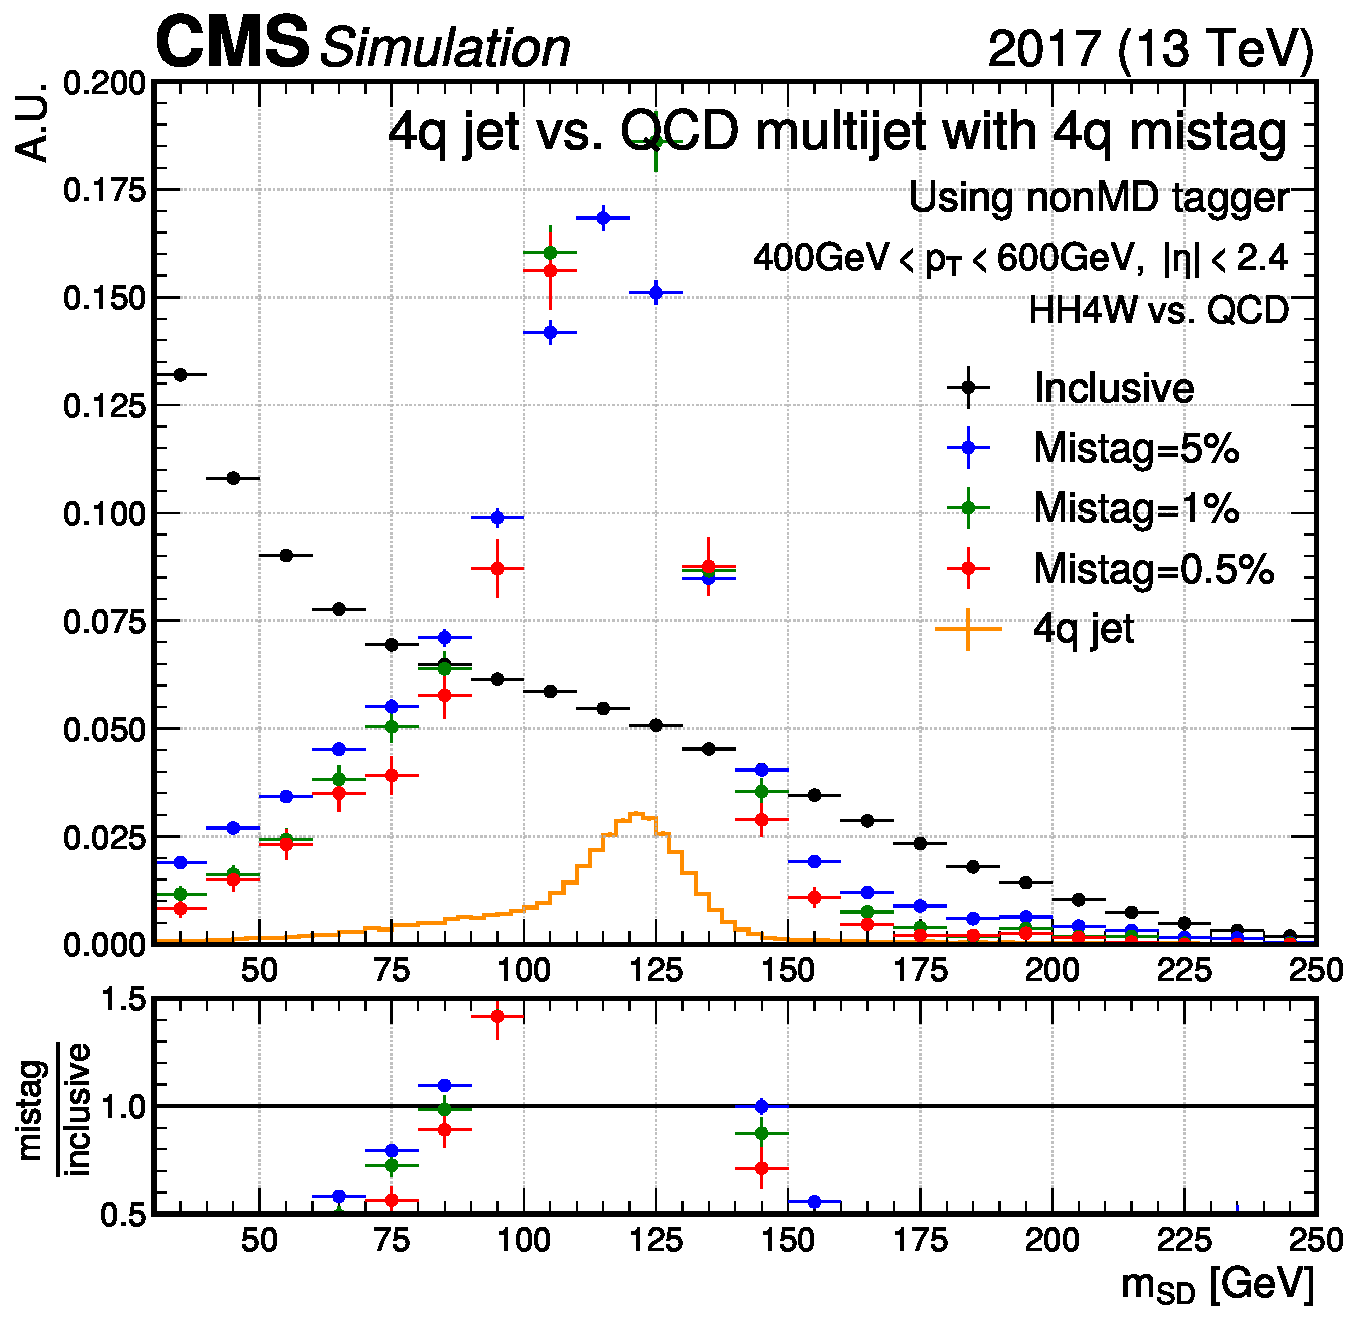
\includegraphics[height=10.5cm, width=10.5cm]{pictures/MD_nonMD_4q.pdf}
 \label{fig:5.4}
\end{figure}

除此之外,原有的PN non-MD只是$H\to W(2q)W(2q)$的单衰变道标记器,但我们开发的标记器是$H\to WW$的多衰变道标记器,所以在其他HWW衰变道上也有用武之地。
\begin{figure}[H]
 \centering
 \caption{被PN nonMD误标记的QCD本底的$m_{SD}$分布}
 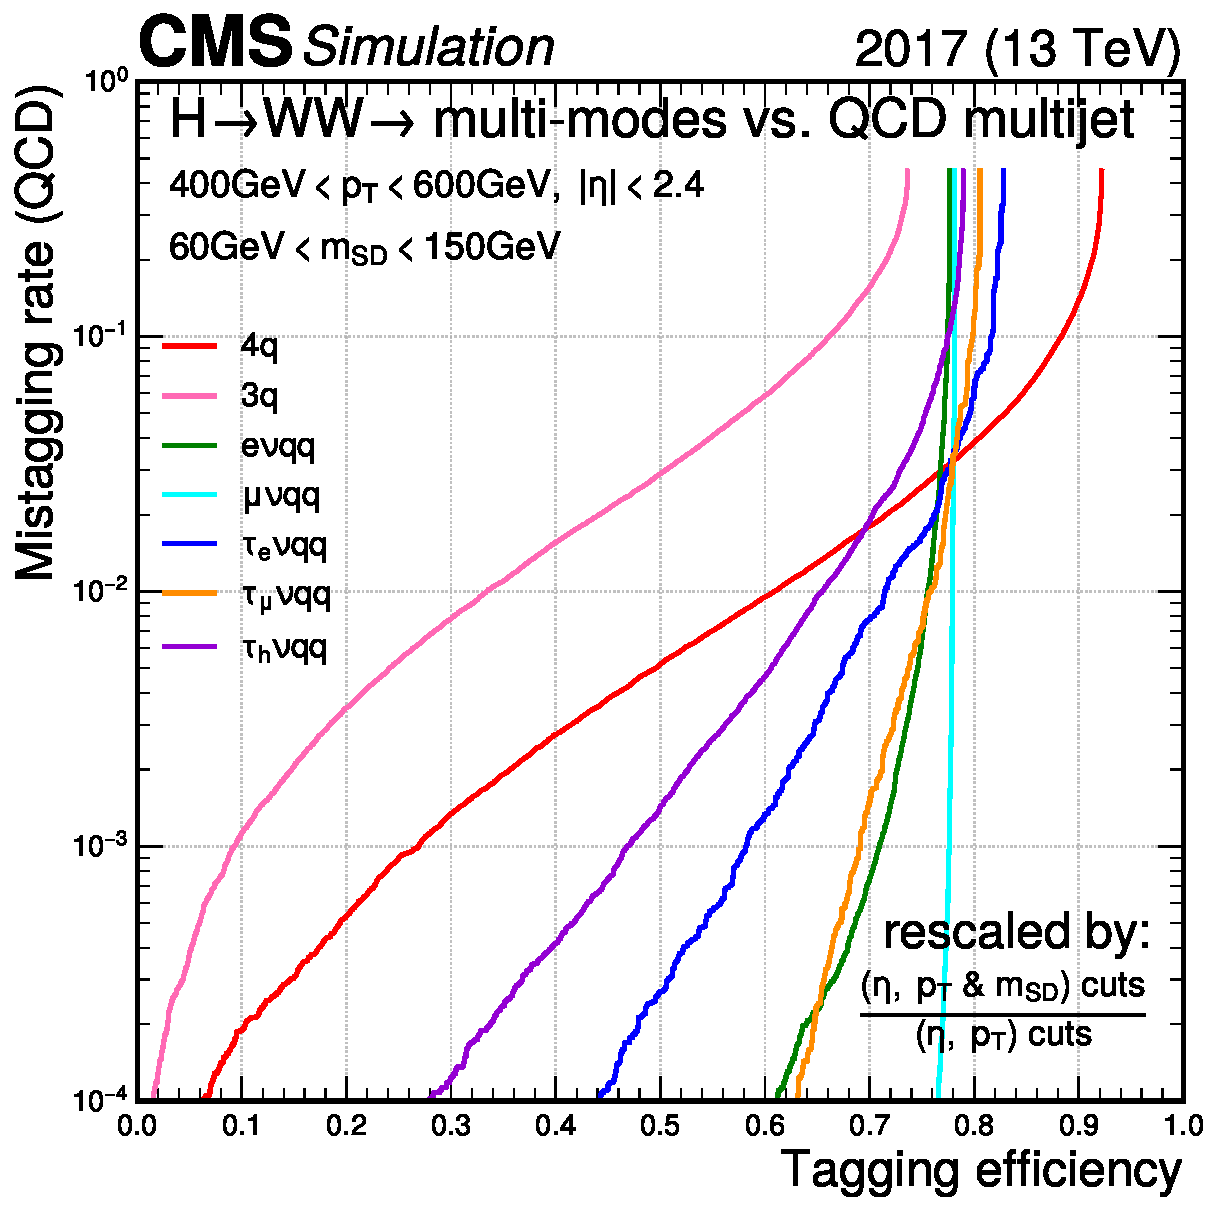
\includegraphics[height=12cm, width=12cm]{pictures/ROC_multi-modes_PKU_std.pdf}
 \label{fig:5.5}
\end{figure}
从这个图里我们可以看到,在Mistag rate=1\%时,除了3q末态(指HWW衰变到四个夸克但只有三个出现在被重建的AK8喷注中)的标记效率只有33\%左右,其他几个道的标记啊效率都在60\%$\sim$80\%之间,更让我们对开发的标记器充满信心。
\section{在分析中的初步应用效果}
我们目前已经将开发的标记器投入正式的CMS实验分析中使用,目前已经应用的分析为:胶子聚合产生希格斯,再到WW散射的过程。在分析探索中,我们把我们的标记器和目前官方分析中针对AK8喷注常用的DeepAK8-MD标记器进行了比较。比较结果如下:


	\chapter{总结和展望}

\fontsize{12bp}{14.4pt}

第六章部分...
    
    \appendix
    \printbibliography[heading = bibintoc]

	\backmatter
	\chapter{致谢}

致谢部分...
	% 需添加二维码
	% Copyright (c) 2008-2009 solvethis
% Copyright (c) 2010-2017,2021 Casper Ti. Vector
% Copyright (c) 2021 Kurapica
% Copyright (c) 2021 iofu728
% All rights reserved.
%
% Redistribution and use in source and binary forms, with or without
% modification, are permitted provided that the following conditions are
% met:
%
% * Redistributions of source code must retain the above copyright notice,
%   this list of conditions and the following disclaimer.
% * Redistributions in binary form must reproduce the above copyright
%   notice, this list of conditions and the following disclaimer in the
%   documentation and/or other materials provided with the distribution.
% * Neither the name of Peking University nor the names of its contributors
%   may be used to endorse or promote products derived from this software
%   without specific prior written permission.
%
% THIS SOFTWARE IS PROVIDED BY THE COPYRIGHT HOLDERS AND CONTRIBUTORS "AS
% IS" AND ANY EXPRESS OR IMPLIED WARRANTIES, INCLUDING, BUT NOT LIMITED TO,
% THE IMPLIED WARRANTIES OF MERCHANTABILITY AND FITNESS FOR A PARTICULAR
% PURPOSE ARE DISCLAIMED. IN NO EVENT SHALL THE COPYRIGHT HOLDER OR
% CONTRIBUTORS BE LIABLE FOR ANY DIRECT, INDIRECT, INCIDENTAL, SPECIAL,
% EXEMPLARY, OR CONSEQUENTIAL DAMAGES (INCLUDING, BUT NOT LIMITED TO,
% PROCUREMENT OF SUBSTITUTE GOODS OR SERVICES; LOSS OF USE, DATA, OR
% PROFITS; OR BUSINESS INTERRUPTION) HOWEVER CAUSED AND ON ANY THEORY OF
% LIABILITY, WHETHER IN CONTRACT, STRICT LIABILITY, OR TORT (INCLUDING
% NEGLIGENCE OR OTHERWISE) ARISING IN ANY WAY OUT OF THE USE OF THIS
% SOFTWARE, EVEN IF ADVISED OF THE POSSIBILITY OF SUCH DAMAGE.

{
	\ctexset{section = {
		format+ = {\centering}, beforeskip = {40bp}, afterskip = {15bp}
	}}
	\specialchap{北京大学学位论文原创性声明和使用授权说明}

	% 学校书面要求本页面不要页码,但在给出的 Word 模版中又有页码。
	% 此处以学校书面要求为准。
	\thispagestyle{empty}
	\mbox{}\vspace*{-3em}
	\section*{原创性声明}

	本人郑重声明:
	所呈交的学位论文,是本人在导师的指导下,独立进行研究工作所取得的成果。
	除文中已经注明引用的内容外,
	本论文不含任何其他个人或集体已经发表或撰写过的作品或成果。
	对本文的研究做出重要贡献的个人和集体,均已在文中以明确方式标明。
	本声明的法律结果由本人承担。
	\vskip 1em
	\rightline{%
		论文作者签名:\hspace{5em}%
		日期:\hspace{2em}年\hspace{2em}月\hspace{2em}日%
	}

	\section*{%
		学位论文使用授权说明\\[-0.33em]
		\textmd{\zihao{5}(必须装订在提交学校图书馆的印刷本)}%
	}

	本人完全了解北京大学关于收集、保存、使用学位论文的规定,即:
	\begin{itemize}
		\item 按照学校要求提交学位论文的印刷本和电子版本;
		\item 学校有权保存学位论文的印刷本和电子版,
			并提供目录检索与阅览服务,在校园网上提供服务;
		\item 学校可以采用影印、缩印、数字化或其它复制手段保存论文;
		\item 因某种特殊原因须要延迟发布学位论文电子版,
			授权学校在 $\Box$\nobreakspace{}一年 /
			$\Box$\nobreakspace{}两年 /
			$\Box$\nobreakspace{}三年以后在校园网上全文发布。
	\end{itemize}
	\centerline{(保密论文在解密后遵守此规定)}
	\vskip 1em
	\rightline{%
		论文作者签名:\hspace{5em}导师签名:\hspace{5em}%
		日期:\hspace{2em}年\hspace{2em}月\hspace{2em}日%
	}

    % 若须排版二维码,请将二维码图片重命名为“barcode”,
    % 二维码内容为: 北京大学 xx学院 xx专业 xxx
    % 容错设置25%
    % 转为合适的图片格式,并放在当前目录下,然后去掉下面 2 行的注释。
    % \vfill\noindent
    % \includegraphics[height = 5em]{barcode}
}

% vim:ts=4:sw=4


\end{document}

% vim:ts=4:sw=4
